\chapter{Evaluation} \label{sec:evaluation}
This chapter presents the results of these evaluations, focusing on the performance improvements achieved through feature fusion compared to baseline models using only transformer embeddings or LIWC features alone.

\section{Initial BERT Finetuning Results}
\begin{table}[H]
\centering
\captionabove[Evaluation of initial BERT base model]{\textbf{Evaluation of BERT base model}}
\label{tab:bert_base}
\begin{tabular}{@{}lrrrrr@{}}
\toprule
Step (Epoch) & Loss & Accuracy & Precision & Recall & \textbf{F1} \\
\cmidrule(lr){2-6} 
3000 (0.52) & 0.007 & 0.998 & 0.999 & 0.998 & \textbf{0.999} \\
9000 (1.57) & 0.003 & 0.999 & 0.100 & 1.000 & \textbf{0.100} \\
15000 (2.61) & 0.004 & 0.999 & 0.999 & 1.000 & \textbf{0.100} \\
17169 (3.00) & 0.002 & 1.000 & 0.999 & 1.000 & \textbf{0.100} \\
\bottomrule
\end{tabular}
\end{table}
As shown in table \ref{tab:bert_base}, the initial BERT fine-tuning on the unmodified PJ and PAN12 datasets achieved \textbf{near-perfect performance, with an F1 score of 0.999 after only 3000 train steps}. This extremely high accuracy suggested that the model was likely exploiting dataset-specific artifacts rather than learning genuine grooming-related patterns. For example, all PJ conversations were labeled as grooming (1) and all PAN12 conversations as non-grooming (0), allowing the model to rely rather on superficial cues such as conversation length or stylistic differences between datasets than on semantic content. This motivated the development of a stricter preprocessing pipeline to mitigate domain leakage and length leakage. In the following sections the improved preprocessing, training and evaluation strategies will be evaluated in detail.

\newpage
\section{Bert Finetuning Results on different Chunk Sizes and Data Setups} \label{sec:bert_chunk_size_and_data_setup}

To evaluate the impact of chunk size and dataset splitting strategy on model performance, a series of experiments were conducted using three different chunk sizes (150, 250 and 512 tokens) and two dataset configurations: a \textit{separated split}, where synthetic non-grooming data was included only in the training set and a \textit{mixed split}, where synthetic data was present in both training and test sets. The chunk distribution and results for each configuration are summarized in the following tables.

\subsection{Fixed Chunk Size of 150 chunks}

\begin{table}[H]
\centering
\small
\caption[Evaluation for Chunk Size 150, Separated Split]{\textbf{Evaluation for chunk size 150, separated split (synthetic data only in train).}}
\label{tab:150_separated}
\begin{tabular}{@{}l *{10}{r} @{}}
\toprule
  & \multicolumn{5}{c}{\textbf{All}} 
  & \multicolumn{4}{c}{\textbf{Real-only}} 
  & \multicolumn{1}{c}{\textbf{Synth-only}} \\
\cmidrule(lr){2-6} \cmidrule(lr){7-10} \cmidrule(lr){11-11}
Step (Epoch) & Loss & Accuracy & Precision & Recall & \textbf{F1}
& Accuracy & Precision & Recall & F1
& Accuracy \\
\midrule
3000 (0.37)  & 0.611 & 0.837 & 0.665 & 0.975 & \textbf{0.790} & 0.949 & 0.897 & 0.975 & 0.934 & 0.231 \\
9000 (1.11)  & 0.555 & 0.859 & 0.696 & 0.981 & \textbf{0.814} & 0.962 & 0.921 & 0.981 & 0.950 & 0.303 \\
15000 (1.85) & 0.529 & 0.872 & 0.719 & 0.976 & \textbf{0.828} & 0.975 & 0.957 & 0.976 & 0.967 & 0.314 \\
21000 (2.59) & 0.498 & 0.888 & 0.747 & 0.973 & \textbf{0.845} & 0.976 & 0.963 & 0.973 & 0.968 & 0.408 \\
24315 (3.00) & 0.553 & 0.869 & 0.710 & 0.985 & \textbf{0.825} & 0.974 & 0.946 & 0.985 & 0.965 & 0.299 \\
\bottomrule
\end{tabular}
\end{table}

\begin{table}[H]
\centering
\small
\caption[Evaluation for Chunk Size 150, Mixed Split]{\textbf{Evaluation for chunk size 150, mixed split (synthetic data in train + test).}}
\label{tab:150_mixed}
\begin{tabular}{@{}lrrrr rr@{}} % = 1 + 5 + 1 + 2 = 9 Spalten
\toprule
  & \multicolumn{5}{c}{\textbf{All}} 
  & \multicolumn{1}{c}{\textbf{Synth-only}} \\
\cmidrule(lr){2-6} \cmidrule(lr){7-7}
Step (Epoch) & Loss & Accuracy & Precision & Recall & \textbf{F1} 
& Accuracy \\
\midrule
3000 (0.36) & 0.352 & 0.939 & 0.870 & 0.992 & \textbf{0.927} & 0.940 \\
9000 (1.07) & 0.257 & 0.975 & 0.958 & 0.979 & \textbf{0.969} & 0.993 \\
15000 (1.79) & 0.253 & 0.977 & 0.968 & 0.974 & \textbf{0.971} & 0.987 \\
21000 (2.50) & 0.248 & 0.980 & 0.965 & 0.986 & \textbf{0.975} & 0.993 \\
25200 (3.00) & 0.255 & 0.979 & 0.957 & 0.989 & \textbf{0.973} & 0.991 \\
\bottomrule
\end{tabular}
\end{table}


\subsection{Fixed Chunk Size of 250 chunks}
\begin{table}[H]
\centering
\small
\caption[Evaluation for Chunk Size 250, Seperated Split]{\textbf{Evaluation for chunk size 250, separated split (synthetic data only in train).}}
\label{tab:250_separated}
\begin{tabular}{@{}lrrrr rr@{}}
\toprule
  & \multicolumn{5}{c}{\textbf{All}} 
  & \multicolumn{1}{c}{\textbf{Synth-only}}  \\
\cmidrule(lr){2-6} \cmidrule(lr){7-7} 
Step (Epoch) & Loss & Accuracy & Precision & Recall & \textbf{F1} & Accuracy \\
\midrule
3000 (0.54) & 0.567 & 0.854 & 0.672 & 0.969 & \textbf{0.793} & 0.158 \\
9000 (1.62) & 0.647 & 0.845 & 0.653 & 0.988 & \textbf{0.786} & 0.082 \\
15000 (2.69) & 0.608 & 0.858 & 0.673 & 0.991 & \textbf{0.802} & 0.145 \\
16704 (3.00) & 0.561 & 0.871 & 0.695 & 0.989 & \textbf{0.816} & 0.200 \\
\bottomrule
\end{tabular}
\end{table}

\begin{table}[H]
\centering
\small
\caption[Evaluation for Chunk Size 250, Mixed Split]{\textbf{Evaluation for chunk size 250, mixed split (synthetic data in test + train).}}
\label{tab:250_mixed}
\begin{tabular}{@{}lrrrr rr@{}}
\toprule
  & \multicolumn{5}{c}{\textbf{All}} 
  & \multicolumn{1}{c}{\textbf{Synth-only}} \\
\cmidrule(lr){2-6} \cmidrule(lr){7-7} 
Step (Epoch) & Loss & Accuracy & Precision & Recall & \textbf{F1} & Accuracy \\
\midrule
3000 (0.52) & 0.298 & 0.958 & 0.903 & 0.988 & \textbf{0.944} & 0.980 \\
9000 (1.57) & 0.255 & 0.976 & 0.941 & 0.996 & \textbf{0.967} & 0.974  \\
15000 (2.61) & 0.242 & 0.984 & 0.964 & 0.993 & \textbf{0.978} & 0.991 \\
17247 (3.00) & 0.242 & 0.984 & 0.962 & 0.994 & \textbf{0.978} & 0.991 \\
\bottomrule
\end{tabular}
\end{table}


\subsection{Fixed Chunk Size of 512 chunks}
\begin{table}[H]
\centering
\small
\caption[Evaluation for Chunk Size 512, Separated Split]{\textbf{Evaluation for chunk size 512, separated split (synthetic data only in train).}}
\label{tab:512_separated}
\begin{tabular}{@{}l *{10}{r} @{}}
\toprule
  & \multicolumn{5}{c}{\textbf{All}} 
  & \multicolumn{4}{c}{\textbf{Real-only}} 
  & \multicolumn{1}{c}{\textbf{Synth-only}} \\
\cmidrule(lr){2-6} \cmidrule(lr){7-10} \cmidrule(lr){11-11} 
Step (Epoch) & Loss & Accuracy & Precision & Recall & \textbf{F1}
& Accuracy & Precision & Recall & F1
& Accuracy \\
\midrule
3000 (0.78)  & 0.472 & 0.894 & 0.690 & 0.989 & \textbf{0.813} & 0.984 & 0.952 & 0.989 & 0.970 & 0.186 \\
6000 (1.55)  & 0.517 & 0.883 & 0.668 & 0.987 & \textbf{0.797} & 0.984 & 0.952 & 0.987 & 0.969 & 0.092 \\
9000 (2.33)  & 0.518 & 0.885 & 0.670 & 0.994 & \textbf{0.800} & 0.982 & 0.941 & 0.994 & 0.967 & 0.116 \\
11610 (3.00) & 0.534 & 0.885 & 0.670 & 0.994 & \textbf{0.801} & 0.985 & 0.951 & 0.994 & 0.972 & 0.093 \\
\bottomrule
\end{tabular}
\end{table}

\begin{table}[H]
\centering
\small
\caption[Evaluation for Chunk Size 512, Mixed Split]{\textbf{Evaluation for chunk size 512, mixed split (synthetic data in train + test).}}
\label{tab:512_mixed}
\begin{tabular}{@{}l *{10}{r} @{}}
\toprule
  & \multicolumn{5}{c}{\textbf{All}} 
  & \multicolumn{4}{c}{\textbf{Real-only}} 
  & \multicolumn{1}{c}{\textbf{Synth-only}} \\
\cmidrule(lr){2-6} \cmidrule(lr){7-10} \cmidrule(lr){11-11}
Step (Epoch) & Loss & Accuracy & Precision & Recall & \textbf{F1}
& Accuracy & Precision & Recall & F1
& Accuracy \\
\midrule
3000 (0.76)  & 0.251 & 0.978 & 0.935 & 0.990 & \textbf{0.962} & 0.978 & 0.938 & 0.990 & 0.964 & 0.970 \\
6000 (1.52)  & 0.282 & 0.970 & 0.907 & 0.995 & \textbf{0.949} & 0.971 & 0.912 & 0.995 & 0.952 & 0.954 \\
9000 (2.28)  & 0.248 & 0.981 & 0.941 & 0.996 & \textbf{0.968} & 0.981 & 0.943 & 0.996 & 0.969 & 0.982 \\
11865 (3.00) & 0.245 & 0.982 & 0.945 & 0.996 & \textbf{0.970} & 0.982 & 0.947 & 0.996 & 0.971 & 0.982 \\
\bottomrule
\end{tabular}
\end{table}


The results of the different chunk sizes and split strategies show that \textbf{BERT generally achieves very high performance on the balanced dataset}, regardless of the chosen chunk size. In addition, the recall is significantly higher than the precision in all runs, indicating that the model correctly identifies almost all grooming cases, but produces some false positives. 

Another notable feature is that the model does not generalize well on synthetic data when it occurs exclusively in the test set. The accuracy in the “synth-only” column remains low in this setting, indicating a distribution shift between real and synthetic data. However, when the proportion of synthetic data is integrated into the training, the effect disappears almost completely and the model learns to successfully incorporate the synthetic data into its decision boundaries.

In addition, it can be seen that the marginal label baseline score increases slightly with increasing chunk size, which is probably due to greater stability of the classifications in longer contexts. Overall, the results confirm that BERT is able to recognize the grooming class almost perfectly, even with a larger context and in a balanced dataset, which is reflected in F1 scores of up to 0.97.

\textbf{Finally, it should be emphasized that the dataset is way more balanced than the original PAN12 dataset (33\% grooming cases vs. only 5\% in PAN12), which explains the excellent metrics. The high data balance leads to clearly separable classes, which further benefits the performance of the model.}


\subsection{Confusion Matrices for BERT Baseline across Chunk Sizes and Data Setups}
%%%%% Confusion Matrices + ROC Curves

\begin{figure}[H]
  \centering

  % --- Erste Reihe: nur Test-Synthetic ---
  \begin{subfigure}[t]{0.32\textwidth}
    \centering
    \includegraphics[width=\linewidth, trim={0 12 0 10},clip]{bert_baseline_plots/sep_synth_in_test/len150/confmat_epoch_03.png}
    \caption{Chunk size = 150 tokens}
  \end{subfigure}\hfill
  \begin{subfigure}[t]{0.32\textwidth}
    \centering
    \includegraphics[width=\linewidth, trim={0 12 0 10},clip]{bert_baseline_plots/sep_synth_in_test/len250/confmat_epoch_03.png}
    \caption{Chunk size = 250 tokens}
  \end{subfigure}\hfill
  \begin{subfigure}[t]{0.32\textwidth}
    \centering
    \includegraphics[width=\linewidth, trim={0 12 0 10},clip]{bert_baseline_plots/sep_synth_in_test/len512/confmat_epoch_03.png}
    \caption{Chunk size = 512 tokens}
  \end{subfigure}

  % --- Zweite Reihe: Train + Test-Synthetic ---
  \vspace{0.4cm}
  \begin{subfigure}[t]{0.32\textwidth}
    \centering
    \includegraphics[width=\linewidth, trim={0 0 0 10},clip]{bert_baseline_plots/mixed/len150/confmat_epoch_03.png}
    \caption{Chunk size = 150 tokens}
  \end{subfigure}\hfill
  \begin{subfigure}[t]{0.32\textwidth}
    \centering
    \includegraphics[width=\linewidth, trim={0 0 0 10},clip]{bert_baseline_plots/mixed/len250/confmat_epoch_03.png}
    \caption{Chunk size = 250 tokens}
  \end{subfigure}\hfill
  \begin{subfigure}[t]{0.32\textwidth}
    \centering
    \includegraphics[width=\linewidth, trim={0 0 0 10},clip]{bert_baseline_plots/mixed/len512/confmat_epoch_03.png}
    \caption{Chunk size = 512 tokens}
  \end{subfigure}

  \caption[Confusion matrices of BERT baseline after epoch 3.]{\textbf{Confusion matrices of the BERT baseline after epoch 3.}  
  Top row: models trained with synthetic data included only in the test set.  
  Bottom row: models trained with synthetic data included in both train and test set.  
  Each column corresponds to a different chunk length (150, 250, 512).}
  \label{fig:bert_confusionmatrices_epoch3}
\end{figure}

Figure \ref{fig:bert_confusionmatrices_epoch3} shows the confusion matrices for the BERT baseline across different chunk sizes and dataset configurations after epoch 3. When looking at the chunk lengths, the false positives and false negatives decrease steadily with an increasing chunk size for both, the false positive and false negative rate and the mixed and seperated data setup. This indicates that the model benefits from a larger context and higher word count, which is consistent with the improved metrics observed in table \ref{tab:bert_base}. It is evident, that the model with the synthetic data in both train and test set achieves a clearly better performance across all chunk sizes with a distingtly lower false positive and also a slightly lower false negative rate across all chunk sizes. This confirms the earlier observation that including synthetic data in training helps the model generalize better to this distribution, leading to fewer misclassifications. 

What is the most striking, is the general higher false positive rate compared to the false negative rate across all configurations. Especially in the setup with the synthetic data only in the test set, the false positive rate is notably higher than the false negative rate (e.g. 1601 FP vs only 18 FN for chunk length 512 tokens), particularly for smaller chunk sizes (e.g. 3864 FP vs 146 FN for chunk length = 150 tokens). Even in the mixed setup, where the performance is generally better, the false positive rate remains slightly higher than the false negative rate. This indicates that the model is generally more conservative in its predictions, preferring to classify uncertain cases as grooming rather than risking missing actual grooming conversations. This behavior is often desirable in practical applications where false negatives (missed grooming cases) can have serious consequences. As already mentioned, the dataset is very balanced, which also contributes to the low false negative rates. Overall, the confusion matrices confirm that BERT performs very well across all configurations, with performance improving with larger chunk sizes and when synthetic data is included in training and with the best performance for chunk size 512 and mixed data setup. \textbf{Note that the values for accuracy, precision and f1 scores are still lower for the mixed setup with chunk size of 512 tokens compared to the mixed setup with chunk size of 250 tokens in table \ref{tab:bert_base}.} This happens because the dataset for 512-token chunks contains fewer samples overall. While the absolute number of false positives and false negatives is lower, their relative share among predictions is higher, which reduces precision. At the same time, recall slightly improves since almost no true positives are missed.


\subsection{ROC Curves for BERT Baseline across Chunk Sizes and Data Setups}

%%%%%%% ROC CURVES

\begin{figure}[H]
  \centering

  % ---------- Top row: synthetic only in TEST ----------
  \begin{subfigure}[t]{0.32\textwidth}
    \centering
    \includegraphics[width=\linewidth]{bert_baseline_plots/sep_synth_in_test/len150/roc_epoch_03_zoom.png}
    \caption{Chunk length = 150}
  \end{subfigure}\hfill
  \begin{subfigure}[t]{0.32\textwidth}
    \centering
    \includegraphics[width=\linewidth]{bert_baseline_plots/sep_synth_in_test/len250/roc_epoch_03_zoom.png}
    \caption{Chunk length = 250}
  \end{subfigure}\hfill
  \begin{subfigure}[t]{0.32\textwidth}
    \centering
    \includegraphics[width=\linewidth]{bert_baseline_plots/sep_synth_in_test/len512/roc_epoch_03_zoom.png}
    \caption{Chunk length = 512}
  \end{subfigure}

  % ---------- Bottom row: synthetic in TRAIN & TEST ----------
  \vspace{0.45cm}
  \begin{subfigure}[t]{0.32\textwidth}
    \centering
    \includegraphics[width=\linewidth]{bert_baseline_plots/mixed/len150/roc_epoch_03_zoom.png}
    \caption{Chunk length = 150}
  \end{subfigure}\hfill
  \begin{subfigure}[t]{0.32\textwidth}
    \centering
    \includegraphics[width=\linewidth]{bert_baseline_plots/mixed/len250/roc_epoch_03_zoom.png}
    \caption{Chunk length = 250}
  \end{subfigure}\hfill
  \begin{subfigure}[t]{0.32\textwidth}
    \centering
    \includegraphics[width=\linewidth]{bert_baseline_plots/mixed/len512/roc_epoch_03_zoom.png}
    \caption{Chunk length = 512}
  \end{subfigure}

  \caption[Zoomed ROC curves after epoch 3 for different chunk lengths.]{\textbf{Zoomed ROC curves after epoch 3 for different chunk lengths (BERT baseline).}
  Top row: models evaluated with synthetic data included \emph{only in the test set} (\(\mathrm{False Positive Rate}\le 0.20\) and \(\mathrm{TPR}\ge 0.90\)). 
  Bottom row: models trained and evaluated with synthetic data in \emph{train \& test} and therefore shown with a \emph{tighter zoom} to expose finer differences (\(\mathrm{False Positive Rate}\le 0.05\) and \(\mathrm{TPR}\ge 0.95\)). 
  Each panel shows the zoomed range of the ROC curve to better reveal separation at low false-positive rates; the legend reports the pAUC for the full ROC.}
  \label{fig:roc_zoom_epoch3}
\end{figure}

Figure \ref{fig:roc_zoom_epoch3} shows the zoomed ROC curves for the BERT baseline across different chunk sizes and dataset configurations after epoch 3. The ROC curves were plotted zoomed for both configurations to highlight the differences more clearly, as the model already performed very well, especially for the mixed dataset, with small differences in the F1 score of < 1\% after epoch 3. \textbf{Note that the zoom levels differ between the two setups.For the setup with synthetic data only in the test set, the ROC curves are shown with a zoom on false positive rates ≤ 0.20 and true positive rates ≥ 0.90, highlighting the overall performance at moderately low FPRs where differences between chunk sizes are still relatively small. For the mixed data setup, a stronger zoom was applied (FPR ≤ 0.05, TPR ≥ 0.95) to emphasize finer distinctions between the models in the critical region, where even small errors become relevant.} 

When looking at the chunk lengths, it is evident that the ROC curves improve steadily with increasing chunk size for both configurations. This indicates that the model benefits from a larger context and higher word count, which is consistent with the improved metrics observed in table \ref{tab:bert_base} and the confusion matrices in figure \ref{fig:bert_confusionmatrices_epoch3}. The pAUC values also increase with chunk size, confirming that larger chunks lead to better overall discrimination between grooming and non-grooming conversations. When comparing the pAUC scores between the two configurations, it is clear that the models trained with synthetic data in both train and test sets achieve significantly higher pAUC values across all chunk sizes. This confirms the earlier observation that including synthetic data in training helps the model generalize better to this distribution, leading to improved performance across the entire ROC curve. Overall, the zoomed ROC curves confirm that BERT performs very well across all configurations, with performance improving with larger chunk sizes and when synthetic data is included in training, consistent with previous analyses.

\section{Comparing LIWC-2022 Macro Groups} \label{sec:global_liwc_analysis}


\begin{figure}[ht]
    \centering
    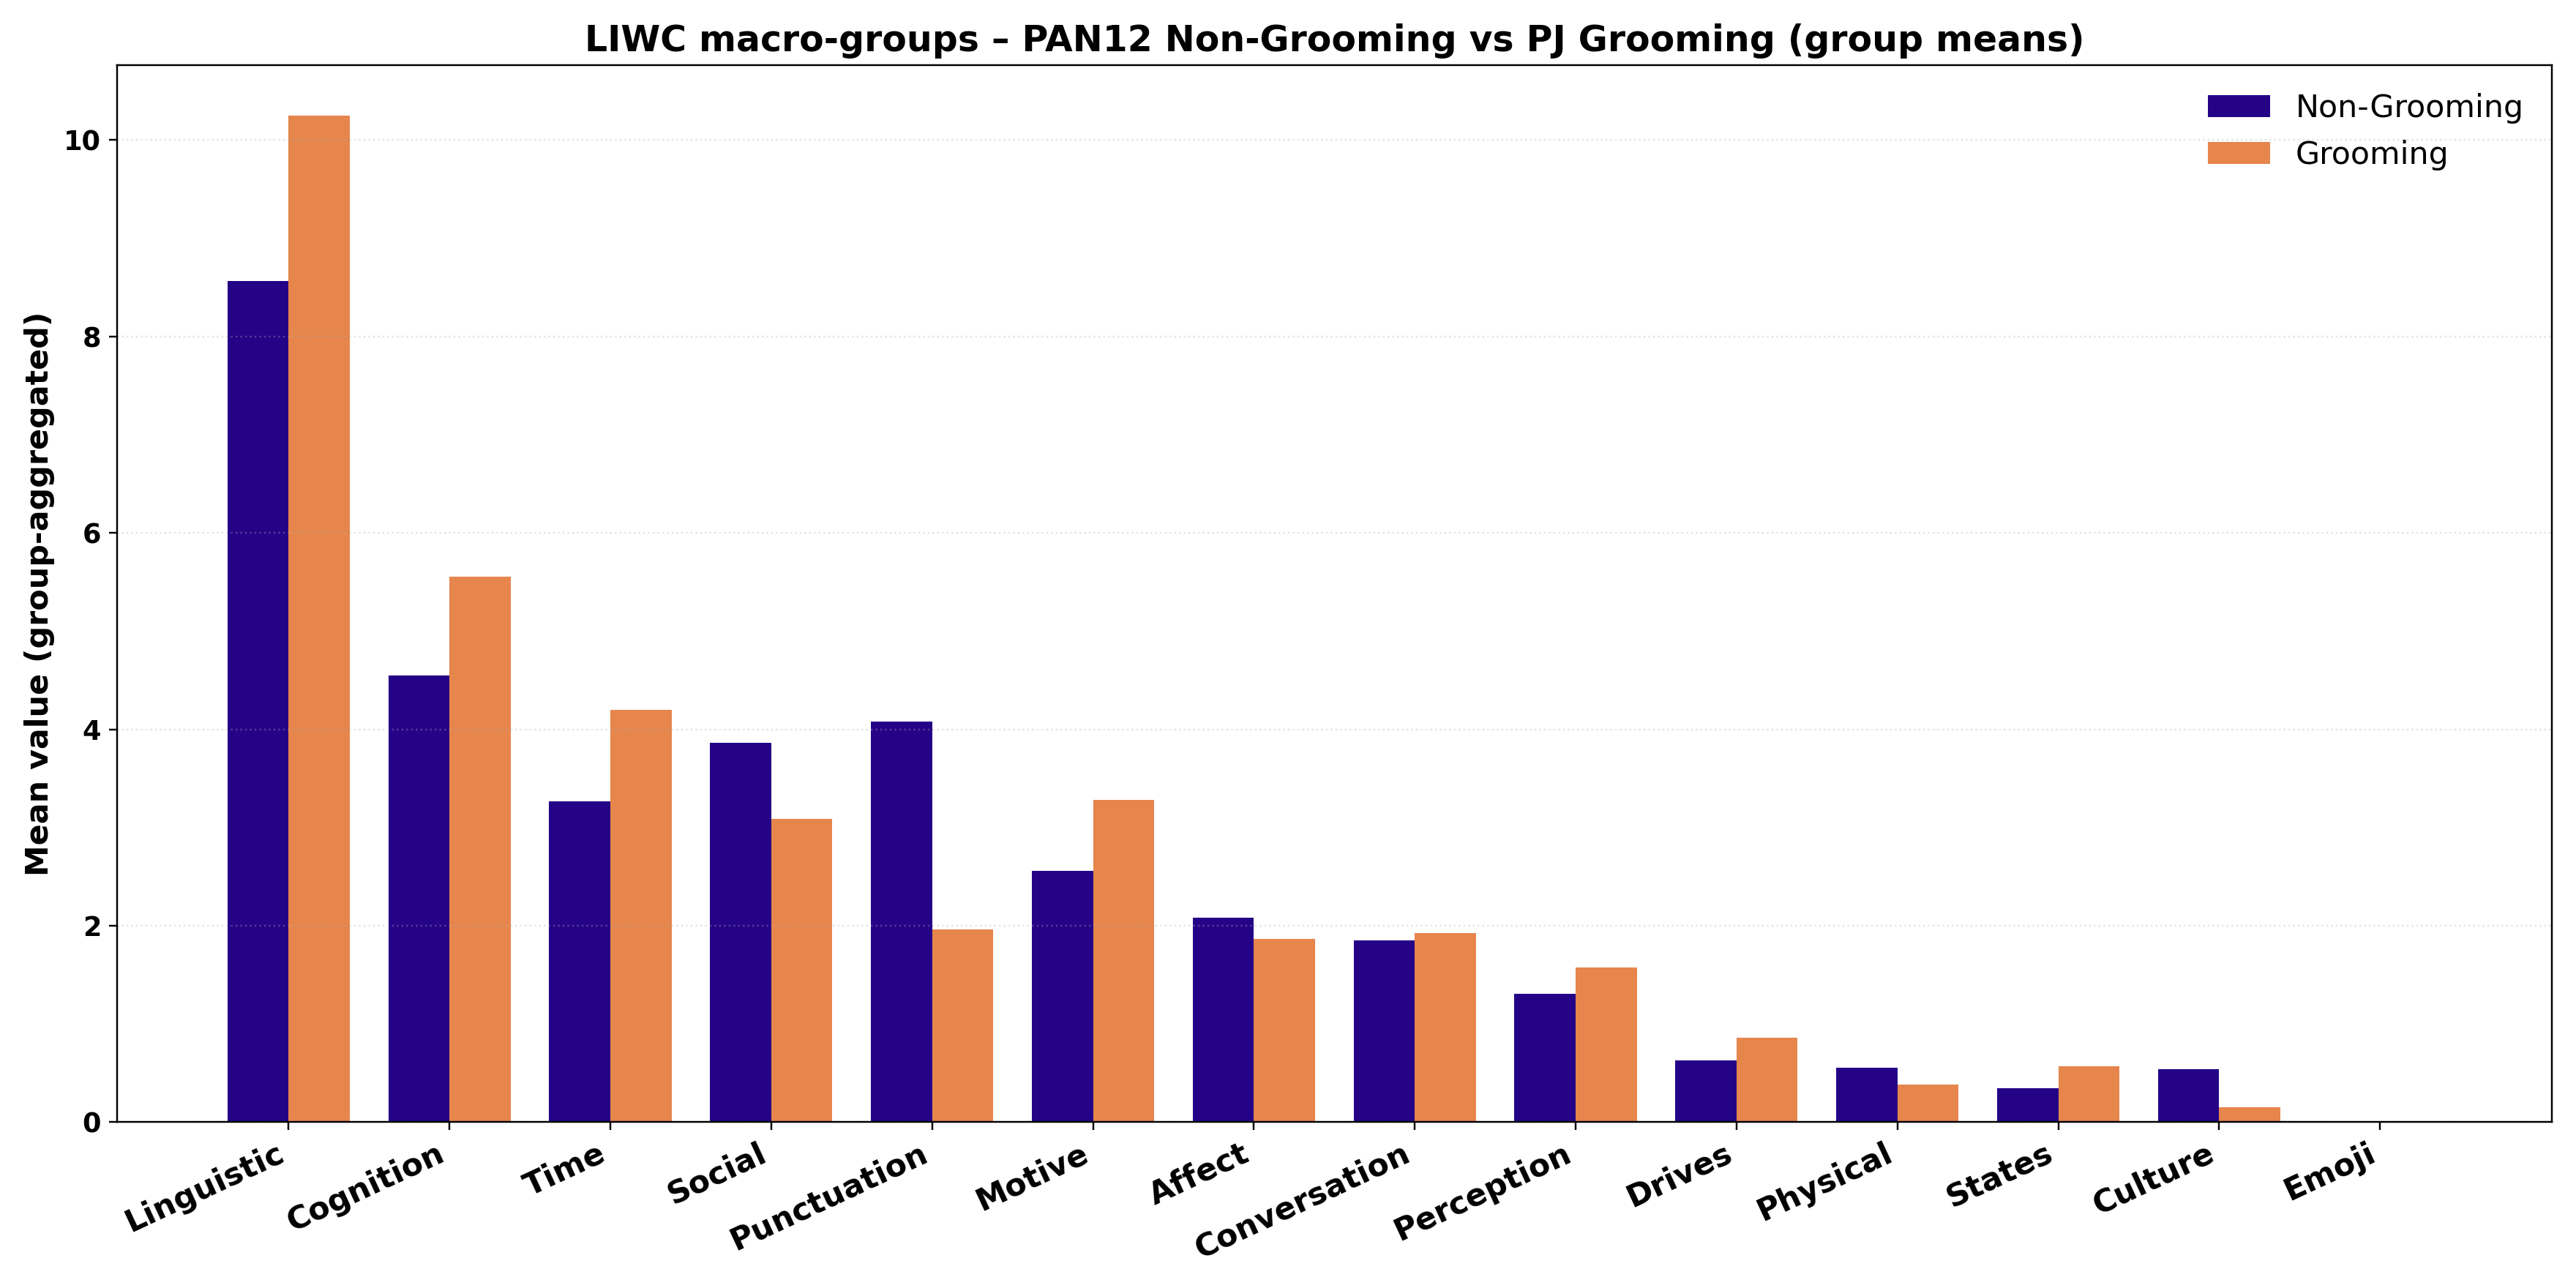
\includegraphics[width=0.90\textwidth]{groups_mean_pan12_vs_pj.png}
    \caption[Comparison of aggregated LIWC macro-groups]{Comparison of aggregated LIWC macro-groups between PAN12 (non-grooming) and PJ (grooming) over global conversations.}
    \label{fig:liwc_macro_groups}
\end{figure}


Figure~\ref{fig:liwc_macro_groups} compares the mean values between the LIWC scores of PAN12 (non-grooming) and PJ (grooming) conversations, aggregated into their Macro Groups.

The results indicate that linguistic features dominate both corpora, with PJ showing significant higher values. \textit{Note that the collected PJ conversations are generally longer and therefore containing more linguistic markers overall.} More interesting is, that the groups \textit{Time}, \textit{Cognition} and \textit{Social} stand out, where PJ conversations show a stronger presence of temporal references (often linked to future planning of meetings), cognitive processes and social markers. Also, the Category ``Emoji´´ hows no Liwc-Values for both Datasets as a result of the slang handling and data preprocssing steps and different kind of emoji usage in the time, the datasets were collected.

Overall, the group-level aggregation highlights the major shifts across all LIWC-dimensions, providing a perspective to the category-wise analysis. This confirms that grooming communication is  characterized not only by increased length and density of language, but also by a distinct emphasis on cognitive, temporal and social processes.


\section{Comparing LIWC Features between PJ and PAN12 on Full Conversations} \label{sec:liwc_global_analysis}

\begin{figure}[ht]
    \centering
    \begin{subfigure}[t]{0.48\textwidth}
        \centering
        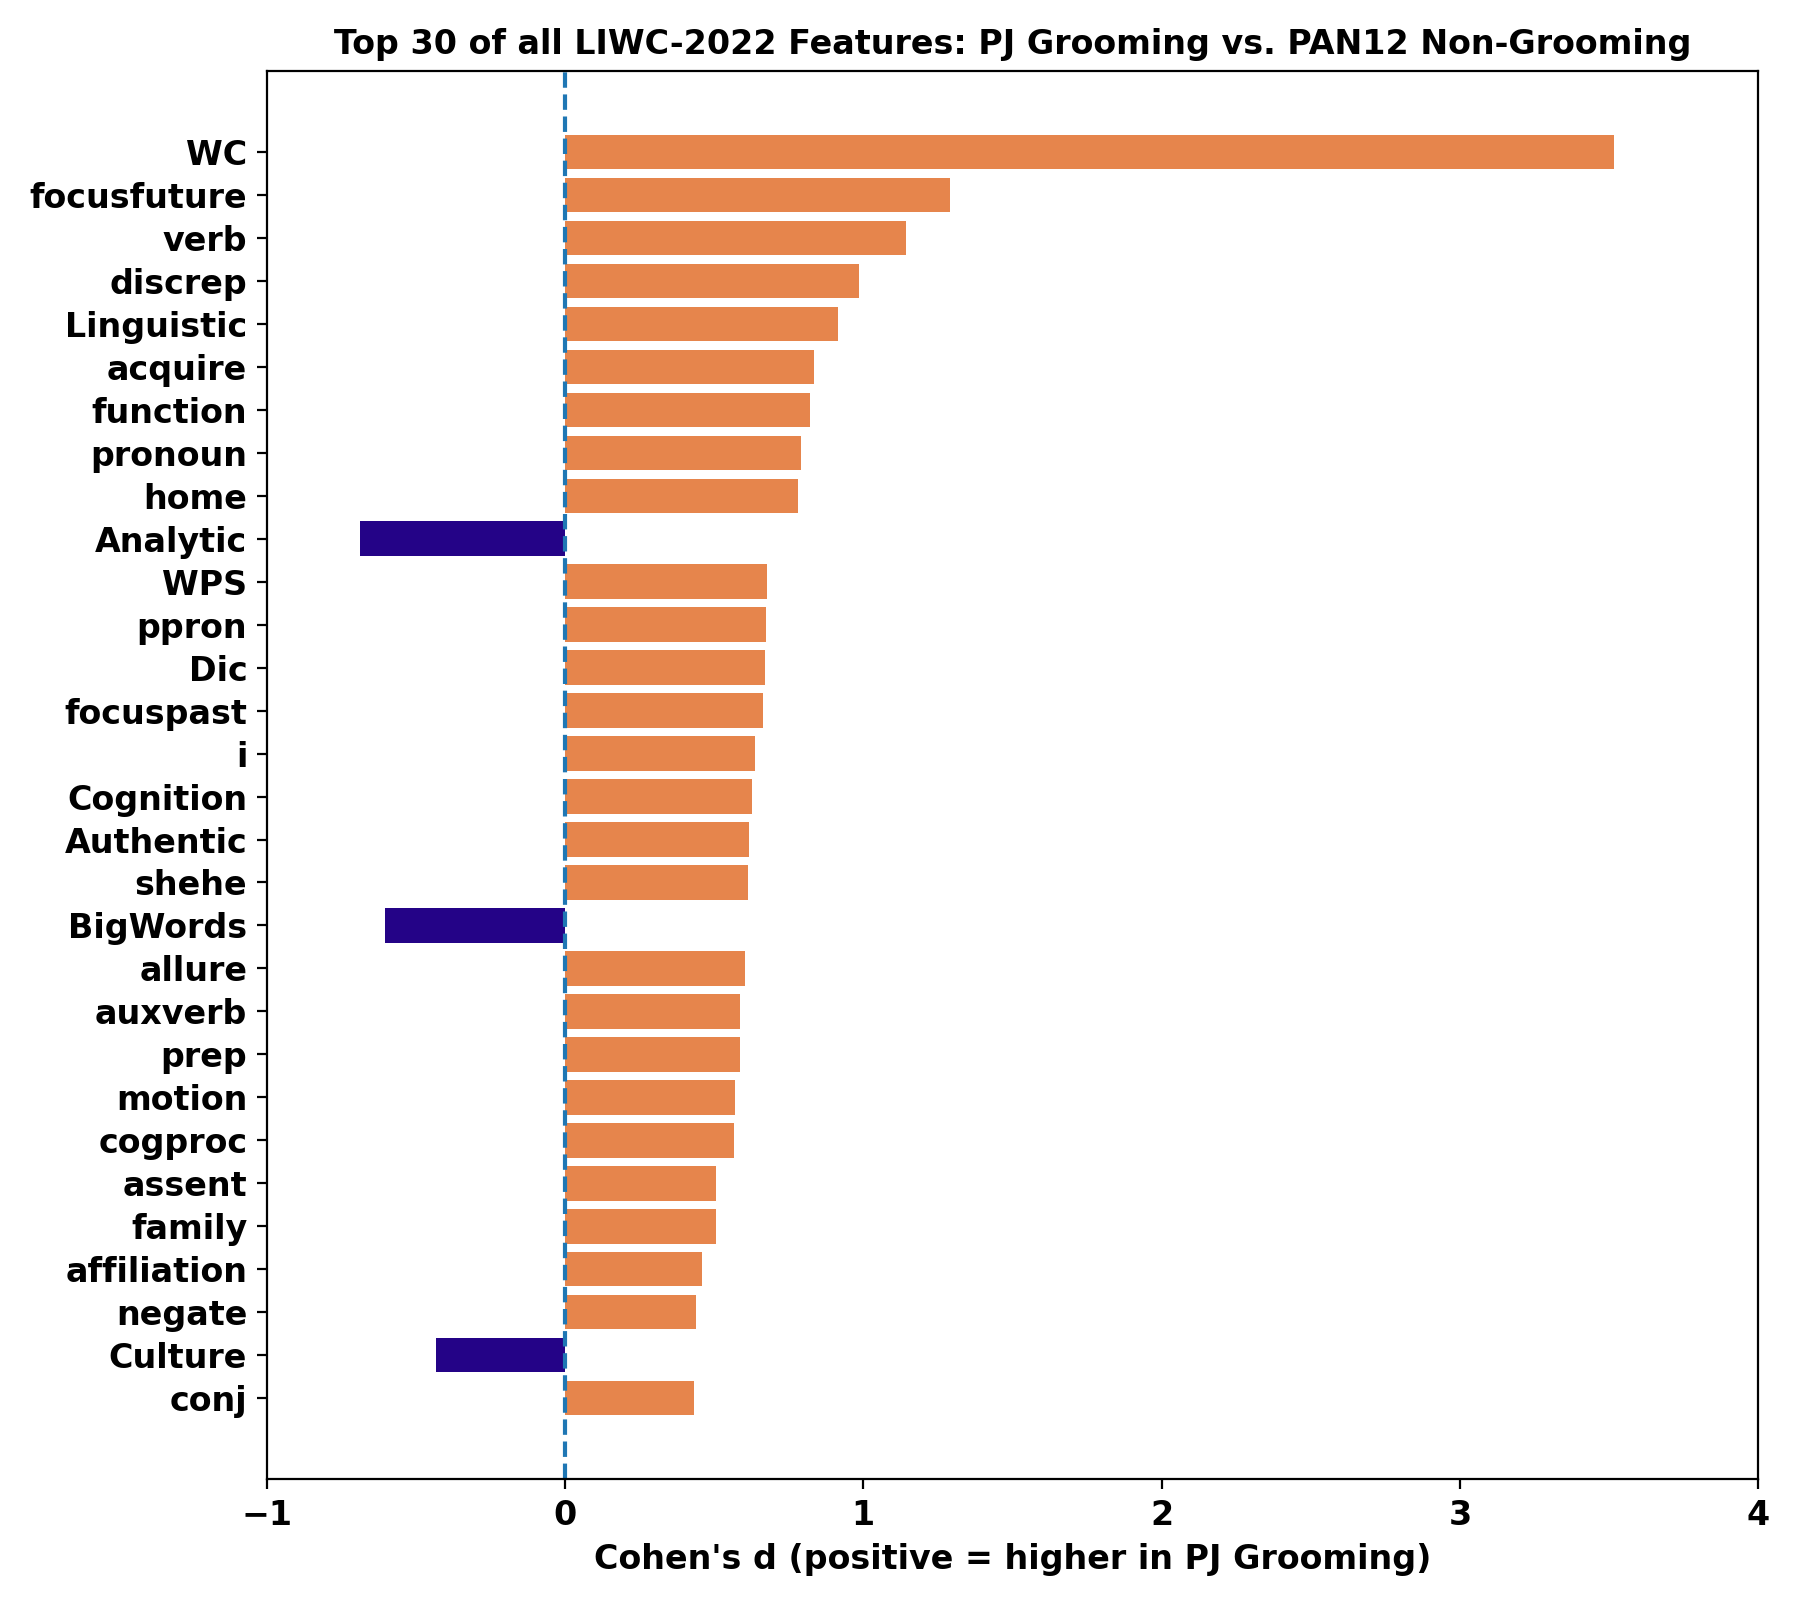
\includegraphics[width=\linewidth]{liwc_top15_d_global.png}
        \caption{Top 30 LIWC categories across all LIWC-2022 features.}
    \end{subfigure}
    \hfill
    \begin{subfigure}[t]{0.48\textwidth}
        \centering
        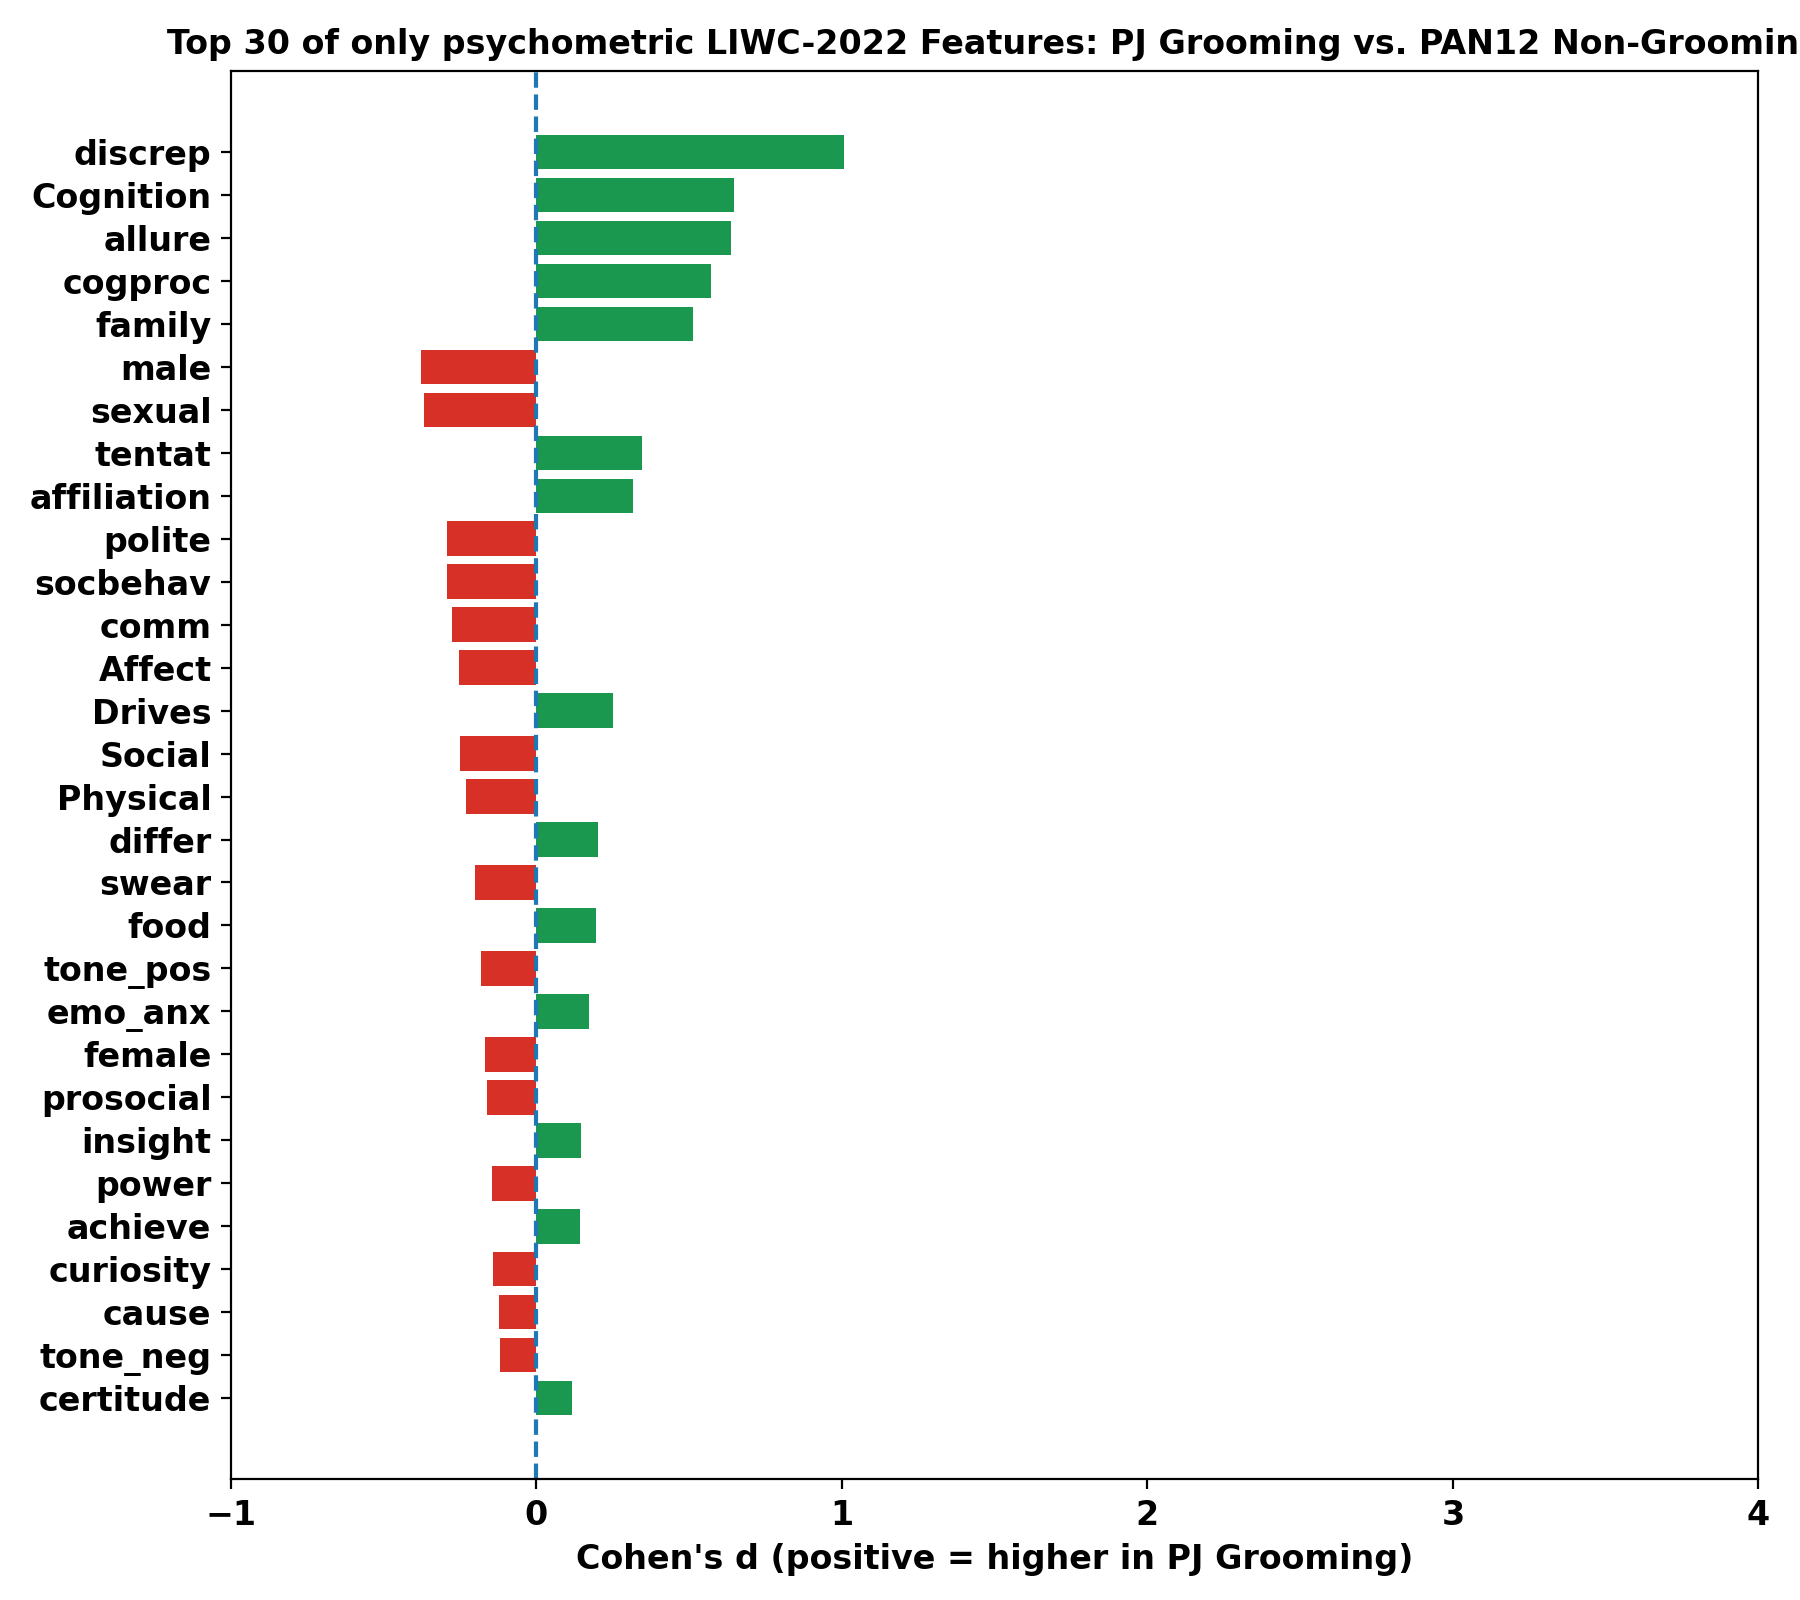
\includegraphics[width=\linewidth]{liwc_top15_d_by_psychometrics.png}
        \caption{Top 30 LIWC-2022 features highlighted in the literature.}
    \end{subfigure}
    \caption[LIWC-Feature Comparison (PJ, PAN12) over Complete Conversations]{LIWC feature comparison between grooming (PJ) and non-grooming (PAN12) dialogues based on cohens $d$ \cite{cohen1988}. Positive values indicate higher feature usage in grooming.}
    \label{fig:liwc_global_analysis}
\end{figure}


In addition, the effect size \textbf{Cohen’s $d$} \cite{cohen1988} was computed to quantify group differences. Figure \ref{fig:liwc_global_analysis} (left) shows the top 30 LIWC features with the largest absolute effect sizes across all LIWC-2022 features, while figure \ref{fig:liwc_global_analysis} (right) focuses on the top 30 features from the psychometric subset highlighted in prior literature (Section \ref{sec:liwc-feature-selection}). For both plots, values over 0 indicate higher feature values in PJ-Grooming conversations, while values below 0 indicate higher values in PAN12 non-grooming conversations. Note, that effect sizes appear lower in the psychometric subset, since it is fully contained within the complete feature set and does not include the strongest differentiating features as shown in the left figure. 

Again, as shown in figure~\ref{fig:liwc_global_analysis} (left), PJ conversations are overall much longer (higher word counts), have longer sentences, and have overall more linguistically features like pronouns, verbs and function words. Since that is a strong confounder, for more content-related interpretations, these features should be ignored. When looking at the dialogical style, many functions words seem to be more prevalent in grooming conversations, which could be related to the more complex sentence structures and higher word counts. Also, the higher word count makes the pj conversations caputure a broader range of topics leading to more diverse linguistic markers.
What is noticeable is the strong presence of the feature \textit{focusfuture}, which reflects the grooming strategy of planning future meetings. Also, next to the linguistic features, the thematic references like \textit{family}, \textit{home} and \textit{affiliation} stand out, being higher present in grooming conversations from PJ than in PAN12, which could also be more consistent with the typical grooming narratives (e.g. asking, if the parents are home). Furthermore, the complexity in grooming conversations tends to be lower than in non-grooming conversations, as indicated by the lower \textit{big words}, \textit{Analytic} and \textit{Culture} score, which could be due to the sources that PAN12 was collected from (e.g. forums, chatrooms) which often containing computer-related and more complex language.

When focusing on the psychometric features (right), the differences between grooming and non-grooming conversations become more pronounced. It is noticeable, that grooming conversations show a higher values in features like \textit{Cogntition}, \textit{cognitive processes} and \textit{Allure} which could be caused by a content related reference to seduction and manipulation. Therefore grooming conversations are clearly distinguishable based on psychological strategies like building closeness (social/affilation), attraction (allure) and cognitive engagement (cognitive processes). Also, the strongest signal of grooming conversations lies in the feature \textit{discrep} (would, should, could), showing a higher presence of words which might be used in boundary testing, conditioning and suggestions. This is accompanied by slight positive effects for \textit{tentant} (hedging) and \textit{polite} (courtesy or relationship building). Additionally, the features \textit{Drives}, \textit{insight}, \textit{achieve} and \textit{emotion anxiety} are more prevalent in grooming conversations, which could be related to the manipulative strategies used by groomers to build trust and emotional connection.
It is striking, that the PAN12 Conversations contain higher values in the features \textit{sexual}, \textit{male/female}, \textit{physical}, \textit{swear} and \textit{Social/social behavior/prosocial}. This is likely due to the fact that the PAN12 dataset contains a considerable amount of sexually explicit but non-grooming conversations for which were included to improve model-robustness. \textbf{Because LIWC computes scores as relative proportions, the shorter PAN12 conversations, which often consist almost entirely of sexual content, produce inflated values in sexual-related categories. In comparison, the longer and more diverse PJ logs dilute these terms within a broader linguistic context, leading to lower proportional scores.} Therefore it should be considered, that the PAN12 dataset is not a perfect representation of non-grooming conversations, but rather a challenging counterbalance to the grooming data. Overall, the LIWC analysis confirms that grooming conversations are characterized not only by increased length and density of language, but also by a distinct emphasis on cognitive, temporal and social processes, as well as specific psychological strategies related to manipulation and relationship building. These insights provide a deeper understanding of the linguistic and psychological markers of grooming behavior, which can inform the development of more effective detection models.


\section{Comparing LIWC Features between PJ and PAN12 and the Synthetic Dataset} \label{sec:liwc_synthetic_comparison}
% Im Text
\begin{figure}[ht]
  \centering
  \begin{subfigure}[t]{0.48\textwidth}
    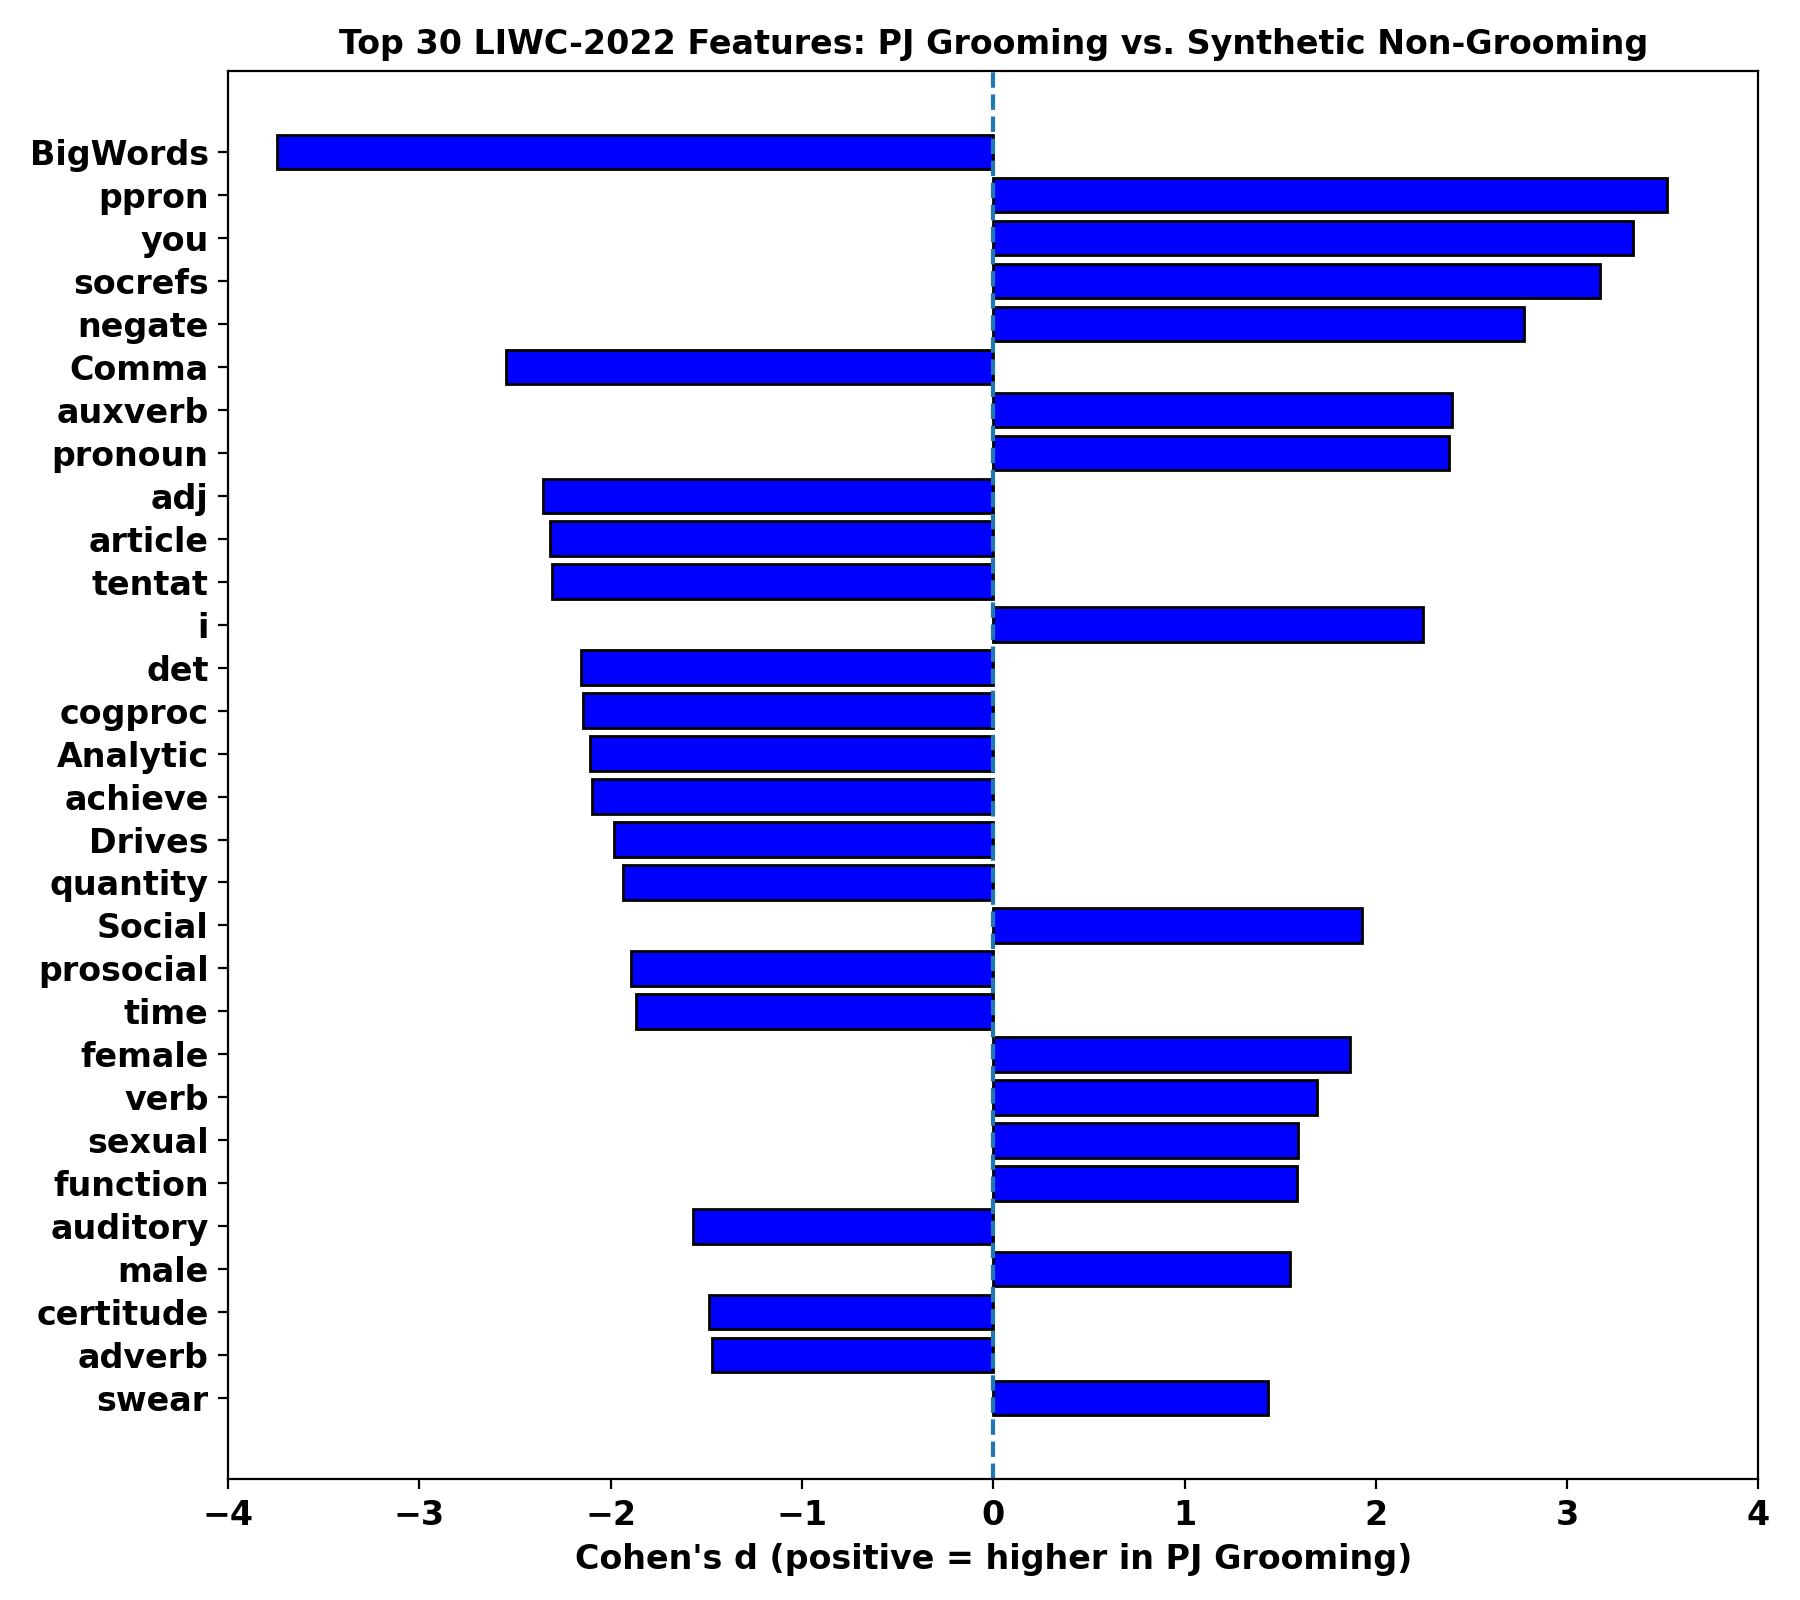
\includegraphics[width=\linewidth]{synthetic_comparison_pj.png}
    \caption{PJ vs. synthetic}
  \end{subfigure}\hfill
  \begin{subfigure}[t]{0.48\textwidth}
    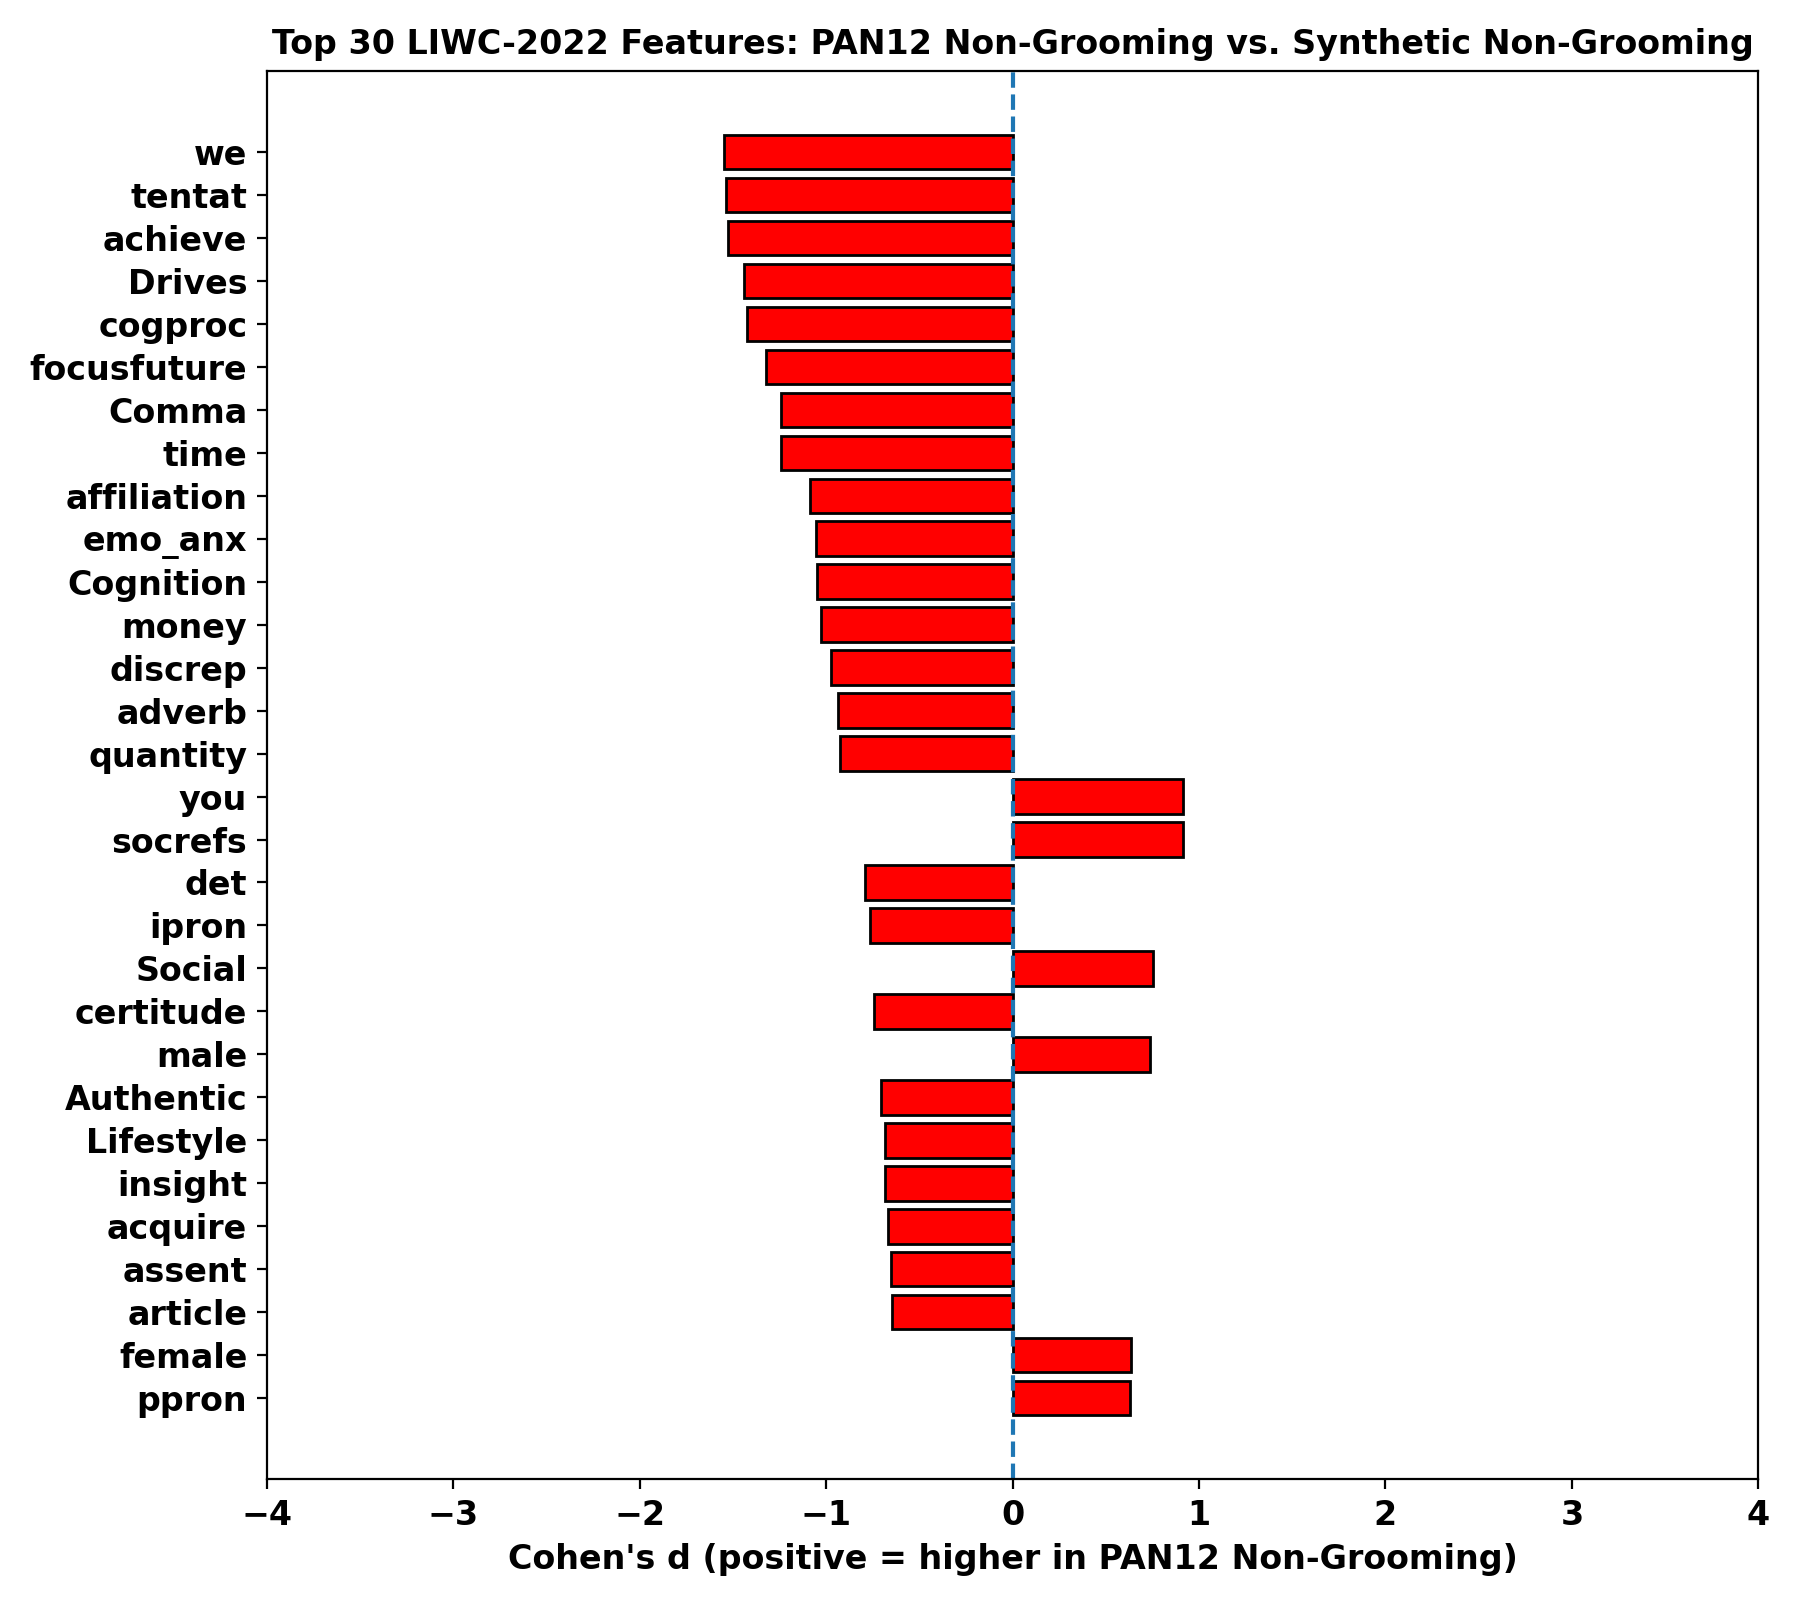
\includegraphics[width=\linewidth]{synthetic_comparison_pan.png}
    \caption{PAN12 vs. synthetic}
  \end{subfigure}
  \caption[Top 30 LIWC Differences with Synthetic Baseline]{Top LIWC differences with synthetic baseline based on cohens $d$ \cite{cohen1988}.}
  \label{fig:liwc_synth_side_by_side}
\end{figure}



Additionally, Figure~\ref{fig:liwc_synth_side_by_side} (left) shows the comparison between PJ and synthetic non-grooming data. Large discrepancies are visible across several LIWC dimensions, including strong positive shifts for all LIWC-categories such as \textit{Big Words}, \textit{ppron} and \textit{you}, suggesting that the synthetic samples over-represent certain linguistic markers.  Figure~\ref{fig:liwc_synth_side_by_side} (right) shows the comparison between PAN12 and the synthetic data. Here, the synthetic data again diverges notably across all LIWC-Categories. This confirms that the synthetic data differs clearly from both real corpora. Including such data in training therefore \textbf{challenges the model to generalize beyond the specific statistical patterns of PJ and PAN12 alone.}While this reduces predictive performance on real data in isolation only marginally, it improves the model’s ability to handle out-of-distribution examples, making the overall model more robust. Still, when interpreting the LIWC-Features of the predicted grooming and non-grooming class a clear distinction between real and synthetic data should be done, since the synthetic data postpones the real distribution in many LIWC-Categories.


\section{Chunk-based LIWC Analysis} \label{sec:chunk_based_liwc_analysis}


%%%% Überarbeitet

\begin{figure}[ht]
    \centering
    \begin{subfigure}[t]{0.49\textwidth}
        \centering
        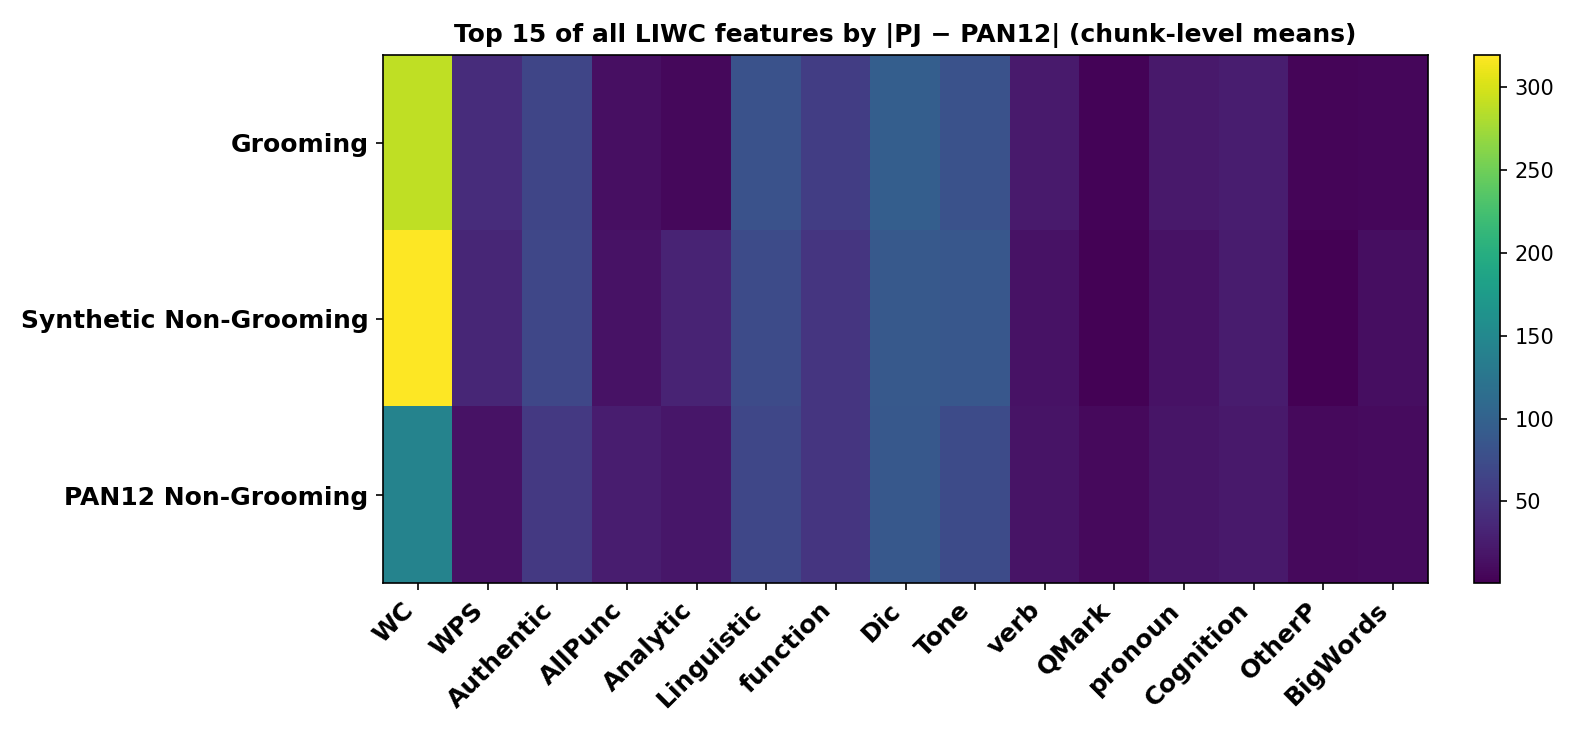
\includegraphics[width=\linewidth]{heatmap_topdiff_gobal.png}
        \caption{Top 15 LIWC categories on 512 chunk-level across all LIWC-2022 features.}
    \end{subfigure}
    \hfill
    \begin{subfigure}[t]{0.49\textwidth}
        \centering
        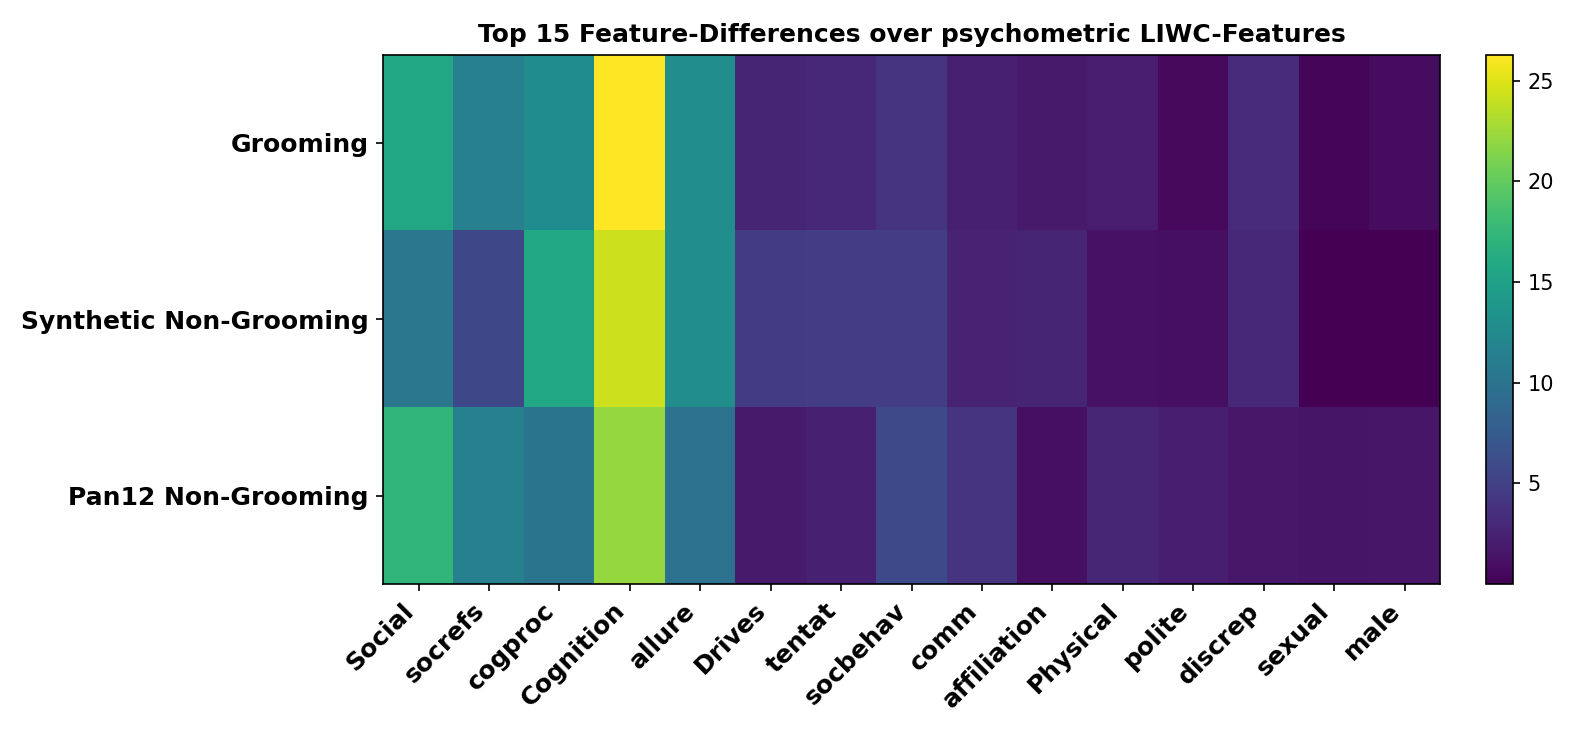
\includegraphics[width=\linewidth]{heatmap_topdiff_psycho.png}
        \caption{Top 15 LIWC-2022 features on 512 chunk-level highlighted in the literature.}
    \end{subfigure}
    \caption[LIWC Feature Comparison at Chunk Level]{LIWC feature comparison between grooming and non-grooming dialogues based on LIWC-2022 Features at chunk level.}
    \label{fig:liwc_chunked_analysis}
\end{figure}

In addition to an analysis of the overall conversations, an analysis of the LIWC features at the chunk level of 512 chunks (as used in the later feature fusion) was performed to analyze local variations across chats. 

Figure \ref{fig:liwc_chunked_analysis} shows a heat map of the top 30 mean features of grooming and non-grooming conversations (left) with the largest difference across all LIWC features and (right) with the largest difference across only the psychometric features highlighted in the literature. Rows represent PJ Grooming, Synthetic Non-Grooming and PAN12 Non-Grooming, while columns represent LIWC features. Color intensity encodes the mean feature value per source. The heatmaps show, that the LIWC-Features differ significantly througout all features and three sources at the chunk level, making it easier to understand how a model can already achieve high performance at this level.

When looking at the full feature set (left), it is noticeable, that the main differences between grooming and (synthetic) non-grooming chunks mainly lie on linguistic features such as \textit{word count}, \textit{WPS}, \textit{function words} and \textit{pronouns}, which are all more prevalent in grooming chunks. This confirms the earlier observation that grooming conversations tend to be longer and more linguistically rich, even at the chunk level. It can be seen, that the synthetic data have a very high word count balance out possible length leakage effects on chunk level. The differences in all other categories are less pronounced, but still visible with the real data seeming to be more similar across all LIWC-Categories than the synthetic data. 

When focusing on the psychometric features (right), the differences between grooming and non-grooming chunks become more pronounced. This could be due to the fact, that the scale of the psychometric features is smaller, making differences more visible since there is no feature like word count dominating the scale. It is noticeable, that grooming chunks show a values in features like \textit{Cogntition}, \textit{cognitive processes} and \textit{Allure} which could be caused by a content related reference to seduction and manipulation. Therefore grooming conversations are clearly distinguishable based on psychological strategies like building closeness (social/affilation), attraction (allure) and cognitive engagement (cognitive processes). It is striking that at the chunk level, the grooming conversations have a higher proportion of sexual words, which can be explained by the higher overall relations of sexual terms in smaller conversation segments. Still, the difference is not as strong as expected from prior work \cite{broome2020psycholinguistic,an2025cybergrooming}, which could be due to the fact that the PAN12 dataset contains a considerable amount of sexually explicit but non-grooming conversations. When comparing the synthetic non-grooming data to the real non-grooming data, it can be seen, that the synthetic data again shows a very different pattern across all psychometric features, confirming that the synthetic data differs clearly from both real corpora. 

This chunk-level perspective complements the global analysis by showing that distinguishing features are not only visible when analyzing entire conversations, but also occur within short text chunks. While the bar charts of the global analysis in Figure \ref{fig:liwc_global_analysis} highlight markers such as word count, pronoun usage and function words, the heat maps show that even locally, grooming dialogues have higher values in many categories. In particular, the dominance of sexual terms becomes apparent at the chunk level, as shorter segments amplify their relative frequency, whereas these signals are diluted in complete conversations due to more diverse linguistic content. At the same time, psychometric dimensions such as cognitive and social processes remain dominant in both analyses, underscoring their theoretical relevance.

Taken together, these results suggest that grooming behavior can be detected in the dataset through both global stylistic patterns and local lexical cues, which explains why BERT already shows very strong performance at the finetuning at chunk level.


\section{Feature Fusion Evaluation}

\begin{table}[H]
\centering
\small
\caption[Evaluation: Feature Fusion with all LIWC-2022 Features]{\textbf{Evaluation: Feature Fusion with all LIWC-2022 Features}}
\label{tab:fusion_all}
\begin{tabular}{@{}lrrrrr@{}} % <-- 6 Spalten (l + 5x r)
\toprule
& \multicolumn{5}{c}{\textbf{Test Set Metrics}} \\
\cmidrule(lr){2-6}
\textbf{Step (Epoch)} & \textbf{Loss} & \textbf{Accuracy} & \textbf{Precision} & \textbf{Recall} & \textbf{F1} \\
\midrule
3000 (0.76)  & 0.234 & 0.985 & 0.959 & 0.989 & \textbf{0.974} \\
6000 (1.52)  & 0.231 & 0.987 & 0.962 & 0.994 & \textbf{0.978} \\
9000 (2.28)  & 0.218 & 0.993 & 0.983 & 0.992 & \textbf{0.987} \\
11865 (3.00) & 0.218 & 0.993 & 0.989 & 0.985 & \textbf{0.987} \\
\bottomrule
\end{tabular}
\end{table}


\begin{table}[H]
\centering
\caption[Evaluation: Feature Fusion with LIWC-2022 Subset]{\textbf{Evaluation: Feature Fusion with Subset of LIWC-2022 Features}}
\small
\label{tab:fusion_subset}
\begin{tabular}{@{}lrrrrr@{}} % <-- 6 Spalten
\toprule
& \multicolumn{5}{c}{\textbf{Test Set Metrics}} \\
\cmidrule(lr){2-6}
\textbf{Step (Epoch)} & \textbf{Loss} & \textbf{Accuracy} & \textbf{Precision} & \textbf{Recall} & \textbf{F1} \\
\midrule
3000 (0.76)  & 0.249 & 0.976 & 0.925 & 0.996 & \textbf{0.959} \\
6000 (1.52)  & 0.221 & 0.991 & 0.983 & 0.985 & \textbf{0.984} \\
9000 (2.28)  & 0.219 & 0.992 & 0.990 & 0.983 & \textbf{0.986} \\
11865 (3.00) & 0.218 & 0.993 & 0.989 & 0.986 & \textbf{0.987} \\
\bottomrule
\end{tabular}
\end{table}

The presented tables \ref{tab:fusion_all} and \ref{tab:fusion_subset} summarize the performance of the feature fusion model that combines BERT embeddings with LIWC-2022 features. Both configurations were evaluated at four training steps (3000, 6000, 9000 and 11865), corresponding to epochs of 0.76, 1.52, 2.28 and 3.00.

\subsection{Using all LIWC-2022 Features}

When using all LIWC-2022 features (Table \ref{tab:fusion_all}), the fusion model achieved an improvement of the F1 score in all training steps of the feature-fusion model, starting from 0.974 at 3000 steps and reaching up to 0.987 at 11865 steps. This indicates that the additional psycholinguistic information provided by the LIWC features helps the model better distinguish between grooming and non-grooming conversations. It is striking, that the precision increased in all training steps from 0.935 to 0.959 at 3000 steps and up to a total difference of 4.4 \% to 0.989 at 11865 steps. This suggests that the fusion model is more effective at reducing false positives, which is crucial in practical applications where misclassifying non-grooming conversations as grooming can have serious consequences. On the other hand, there was a small decrease in recall from 0.990 to 0.989 at 3000 steps and from 0.996 to 0.985 at 11865 steps, indicating that the model is slightly less sensitive in identifying all grooming cases. This leads to the conclusion, that the fusion model is more conservative in its predictions using additional LIWC features, which may be beneficial in reducing false alarms while still maintaining high overall accuracy.


\subsection{Using a Subset of Psychometric LIWC-2022 Features}

When using only a subset of psychometric LIWC-2022 features (table \ref{tab:fusion_subset}), the same trend of improvement in F1 score was observed, starting from 0.959 at 3000 steps and reaching up to 0.987 at 11865 steps. This indicates that even a targeted selection of psycholinguistically relevant features can significantly enhance model performance. The precision also showed a substantial increase from 0.925 to 0.959 at 3000 steps and up to 0.989 at 11865 steps, similar to the results when using all features. This reinforces the idea that psychometric features are particularly valuable in improving the model's ability to correctly identify grooming conversations while minimizing false positives. However, the recall showed a slight decrease from 0.996 to 0.985 at 6000 steps and from 0.983 to 0.986 at 11865 steps, indicating a minor trade-off in sensitivity. Overall, the results suggest that even a focused set of psychometric LIWC features can provide benefits when fused with BERT embeddings, enhancing the model's robustness and reliability in detecting grooming behavior.


\subsection{Confusion Matrices for Feature Fusion Models}


\begin{figure}[H]
  \centering

  % -------- Top row: Feature fusion with ALL LIWC-2022 features --------
  \begin{subfigure}[t]{0.32\textwidth}
    \centering
    % \includegraphics[width=\linewidth,trim={0 10 0 28},clip]{fusion_all_epoch01_confmat.png}
    \includegraphics[width=\linewidth]{plots_feature_fusion_all/fusion_eval_epoch_1/confusion_matrix_all_thr_0.50.png}
    \caption{Epoch 1}
    \label{fig:ff_all_e1}
  \end{subfigure}\hfill
  \begin{subfigure}[t]{0.32\textwidth}
    \centering
    \includegraphics[width=\linewidth]{plots_feature_fusion_all/fusion_eval_epoch_2/confusion_matrix_all_thr_0.50.png}
    \caption{Epoch 2}
    \label{fig:ff_all_e2}
  \end{subfigure}\hfill
  \begin{subfigure}[t]{0.32\textwidth}
    \centering
    \includegraphics[width=\linewidth]{plots_feature_fusion_all/fusion_eval_epoch_3/confusion_matrix_all_thr_0.50.png}
    \caption{Epoch 3}
    \label{fig:ff_all_e3}
  \end{subfigure}

  \vspace{0.45cm}

  % -------- Bottom row: Feature fusion with PSYCHOMETRIC subset --------
  \begin{subfigure}[t]{0.32\textwidth}
    \centering
    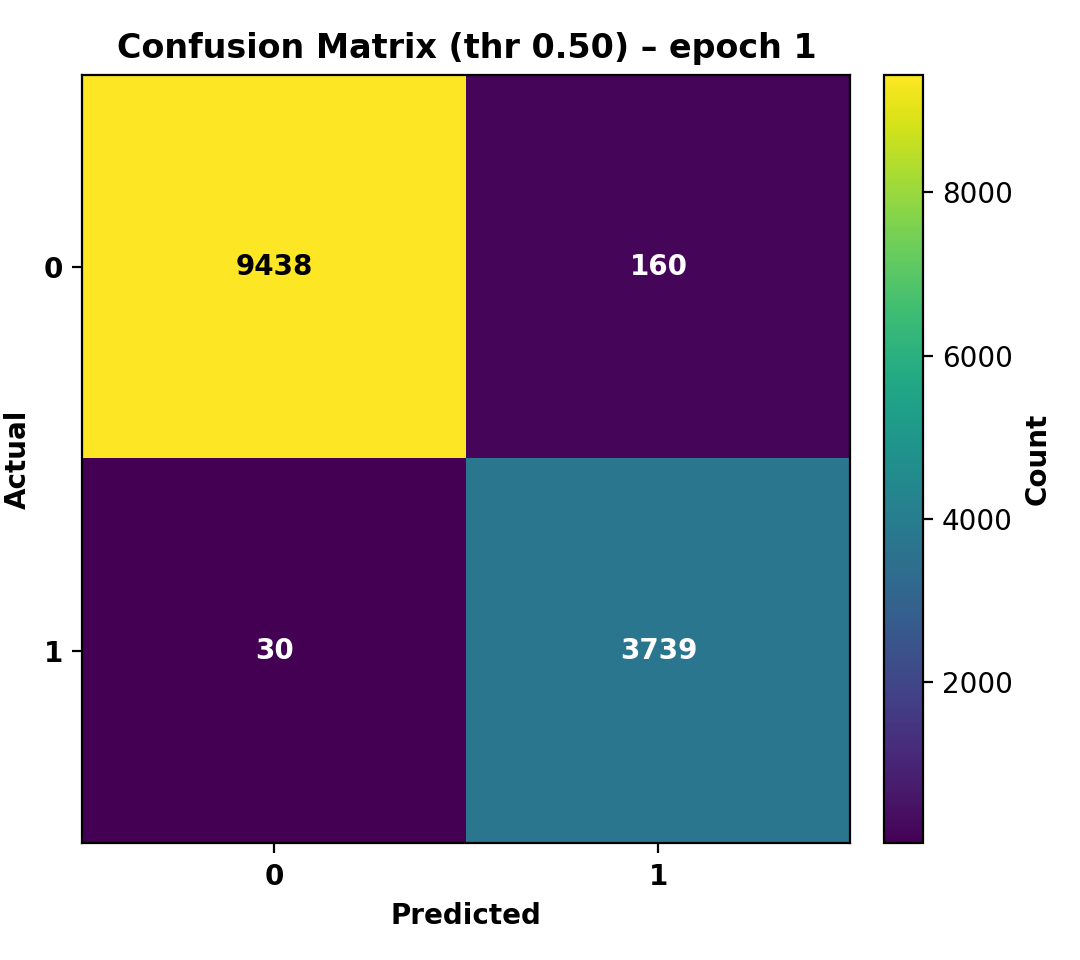
\includegraphics[width=\linewidth]{plots_feature_fusion_subset/epch_1_plots/confmat_thr_0.50_epoch_1.png}
    \caption{Epoch 1}
    \label{fig:ff_psy_e1}
  \end{subfigure}\hfill
  \begin{subfigure}[t]{0.32\textwidth}
    \centering
    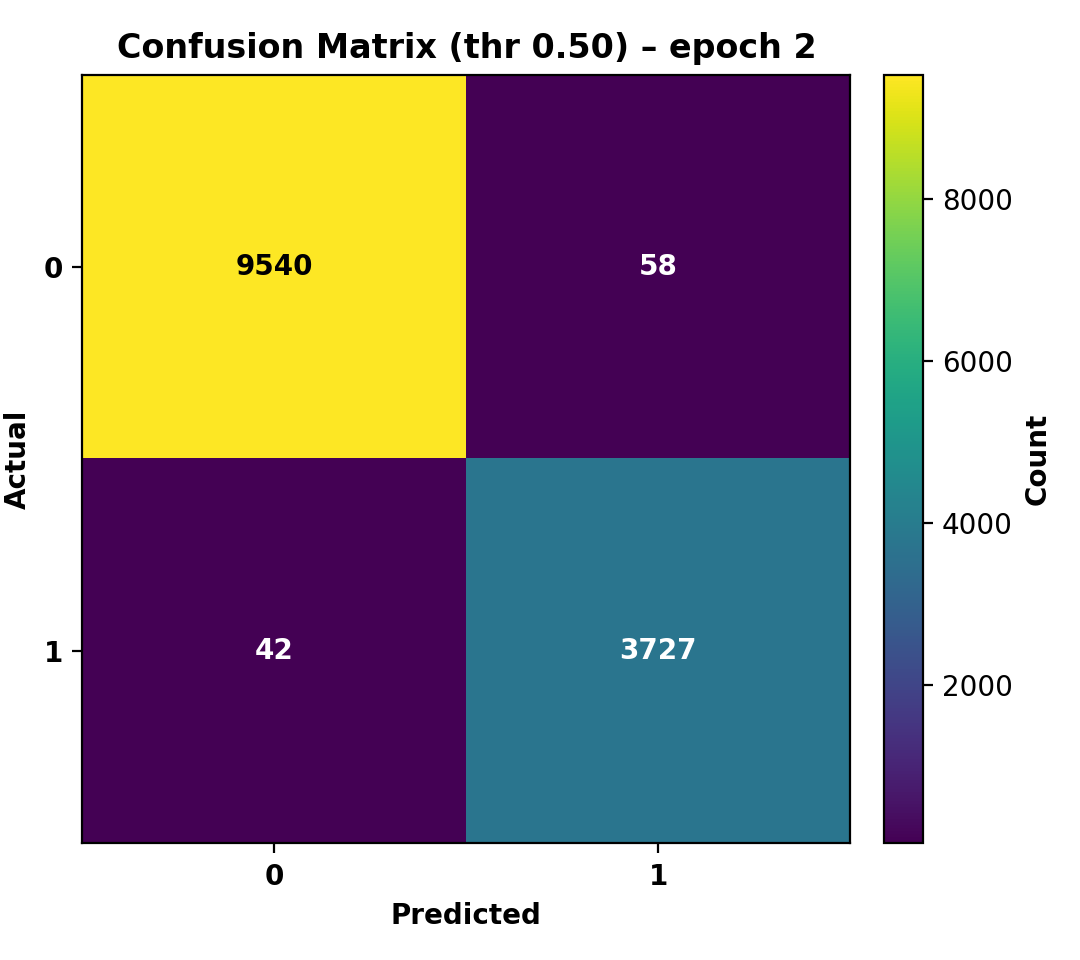
\includegraphics[width=\linewidth]{plots_feature_fusion_subset/epoch_2_plots/confmat_thr_0.50_epoch_2.png}
    \caption{Epoch 2}
    \label{fig:ff_psy_e2}
  \end{subfigure}\hfill
  \begin{subfigure}[t]{0.32\textwidth}
    \centering
    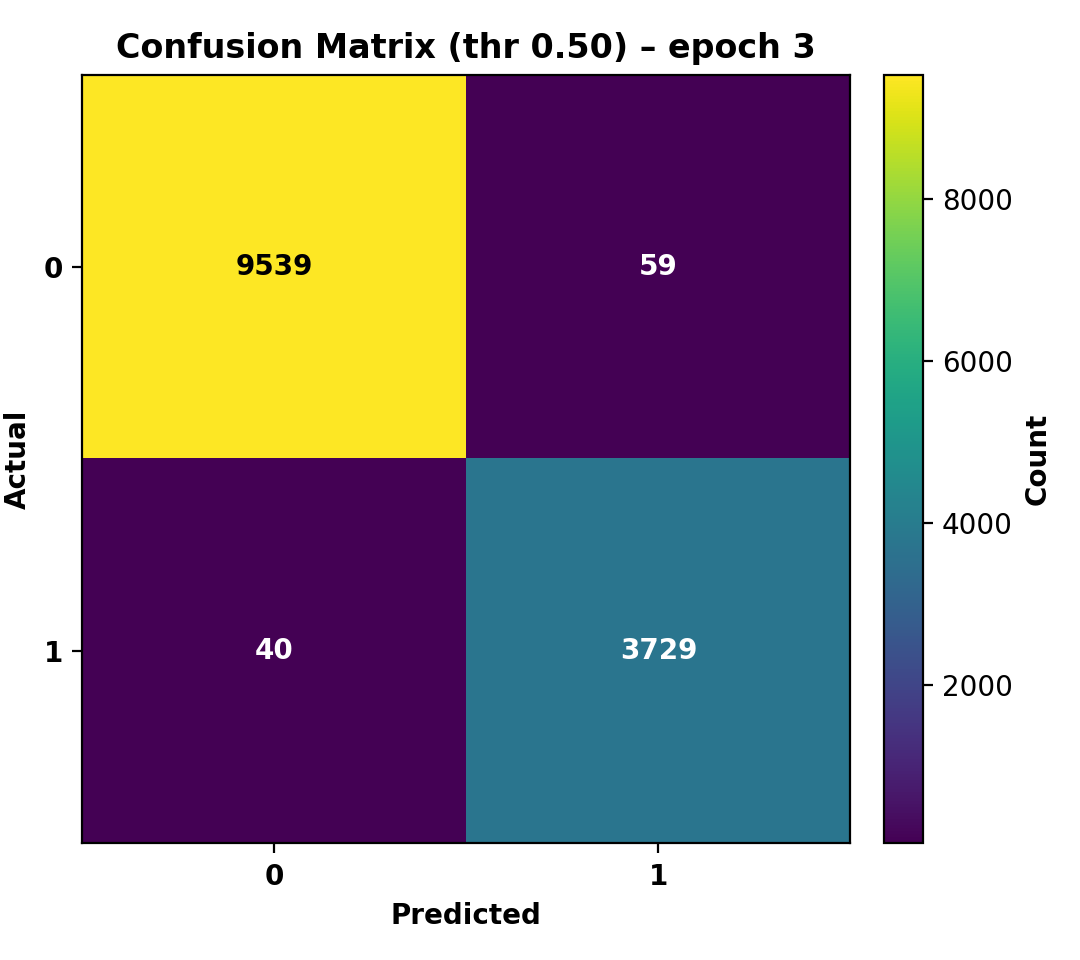
\includegraphics[width=\linewidth]{plots_feature_fusion_subset/epoch_3_plots/confmat_thr_0.50_epoch_3.png}
    \caption{Epoch 3}
    \label{fig:ff_psy_e3}
  \end{subfigure}

  \caption[Confusion matrices by epoch for feature-fusion models.]{\textbf{Confusion matrices by epoch for feature-fusion models (BERT baseline).}
  \emph{Top row:} fusion with all LIWC-2022 features. \emph{Bottom row:} fusion with the psychometric LIWC-2022 subset.
  Each panel shows true labels (rows) vs. predicted labels (columns); diagonal cells indicate correct predictions, off-diagonal cells are errors. The confusion matrices were generated using a classification threshold of 0.5.
  For fair visual comparison, keep the same color scale across all panels.}
  \label{fig:ff_confmats_epochs}
\end{figure}

Figure \ref{fig:ff_confmats_epochs} shows the confusion matrices for both feature-fusion configurations across three epochs. It is notable that both configurations achieve a very balanced performance, having very high true positive rates (TPR) and true negative rates (TNR), with stable values across all epochs, indicating excellent overall classification performance. The number of false positives (FP) and false negatives (FN) is very low in all cases, demonstrating that the models are effective at minimizing both types of errors. 

When comparing the two configurations, it is evident that the model using all LIWC-2022 features shows a slightly better performance in epoch 1, with fewer false positives and false negatives compared to the model using only the psychometric subset. However, as training progresses to epochs 2 and 3, the differences between the two configurations become negligible, with both achieving nearly identical performance in epoch 3. This suggests that while the additional LIWC features may provide some initial benefit, the psychometric subset is sufficient for achieving high accuracy once the model has been adequately trained. Consequently, the confusion matrices reveal that both models maintain high sensitivity and specificity across all three epochs of training and for both configurations (all LIWC-Features and only psychometric subset of features). This suggests that the feature-fusion approach effectively balances the trade-off between detecting grooming conversations and avoiding false alarms. Also, when comparing the feature fusion models to the BERT-Baseline with 512 Chunks and a mixed split \ref{fig:bert_confusionmatrices_epoch3}, it is evident, that the feature fusion models achieve a smaller false positive rate, indicating a more "conservative" classification behavior, which is particularly important in practical applications where false alarms can have serious consequences. However, as already shown in table \ref{tab:fusion_all} and \ref{tab:fusion_subset}, there is a small increase in the false positive rate, indicating a minor trade-off in sensitivity. Still, the differences are relatively small, suggesting that while LIWC features provide additional value, the BERT embeddings already capture much of the relevant information. Overall, the results suggest that the feature-fusion approach is better in classifying non-grooming conversations directly but with a small increase in the false negative rate but an overall more balanced performance than the BERT baseline.


\subsection{ROC Curves for Feature Fusion Models}

%%%%%% ROC CURVES

\begin{figure}[H]
  \centering

  % -------- Top row: Feature fusion with ALL LIWC-2022 features --------

  % -------- Bottom row: Feature fusion with PSYCHOMETRIC subset --------
  \begin{subfigure}[t]{0.32\textwidth}
    \centering
    \includegraphics[width=\linewidth]{plots_feature_fusion_all/fusion_eval_epoch_1/roc_curve_all_zoom.png}
    \caption{Epoch 1}
    \label{fig:ffroc_psy_e1}
  \end{subfigure}\hfill
  \begin{subfigure}[t]{0.32\textwidth}
    \centering
    \includegraphics[width=\linewidth]{plots_feature_fusion_all/fusion_eval_epoch_2/roc_curve_all_zoom.png}
    \caption{Epoch 2}
    \label{fig:ffroc_psy_e2}
  \end{subfigure}\hfill
  \begin{subfigure}[t]{0.32\textwidth}
    \centering
    \includegraphics[width=\linewidth]{plots_feature_fusion_all/fusion_eval_epoch_3/roc_curve_all_zoom.png}
    \caption{Epoch 3}
    \label{fig:ffroc_psy_e3}
  \end{subfigure}

    \vspace{0.45cm}


    \begin{subfigure}[t]{0.32\textwidth}
    \centering
    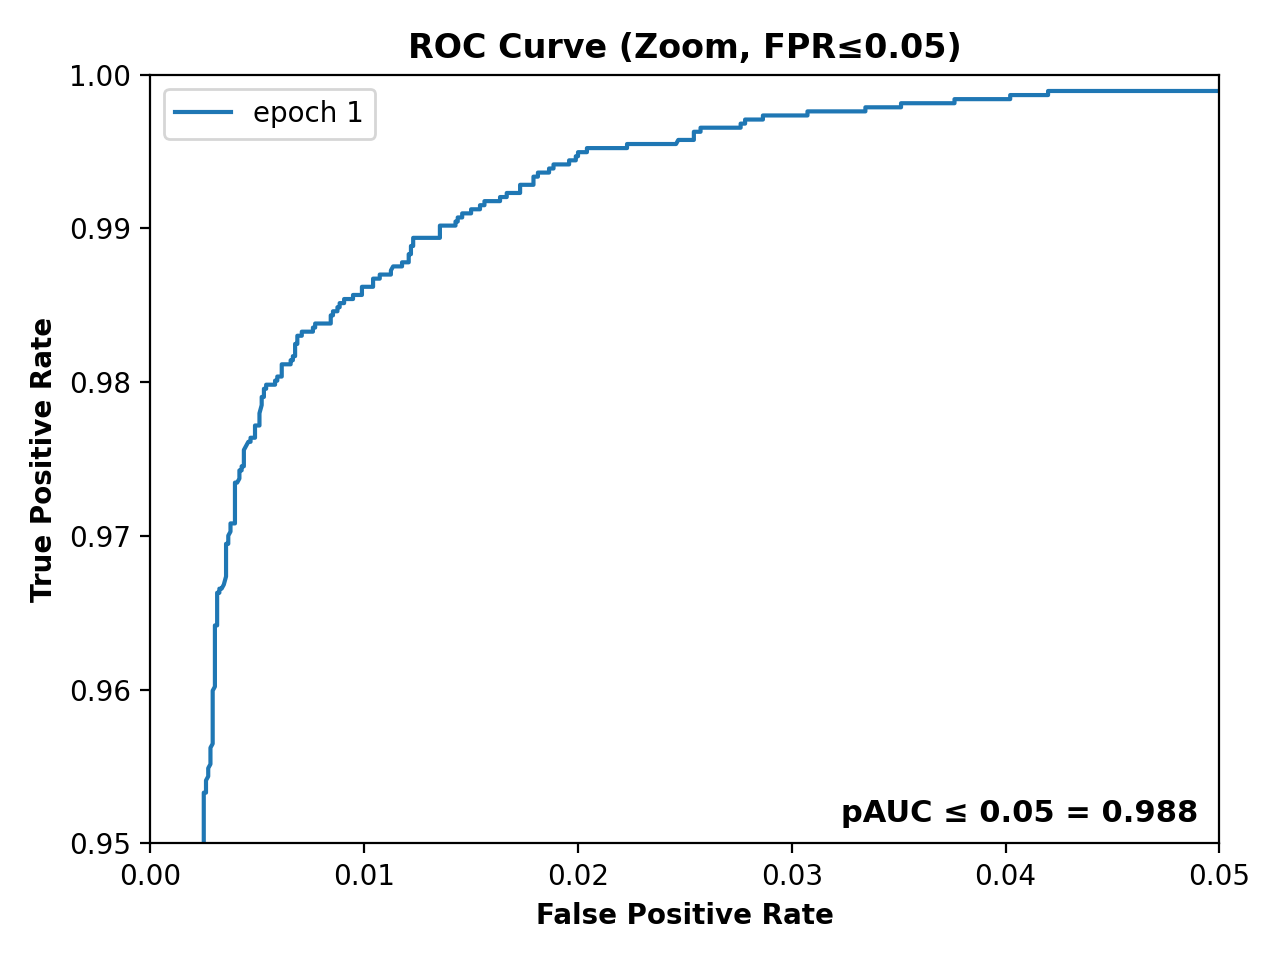
\includegraphics[width=\linewidth]{plots_feature_fusion_subset/epch_1_plots/roc_zoom_epoch_1.png}
    \caption{Epoch 1}
    \label{fig:ffroc_all_e1}
  \end{subfigure}\hfill
  \begin{subfigure}[t]{0.32\textwidth}
    \centering
    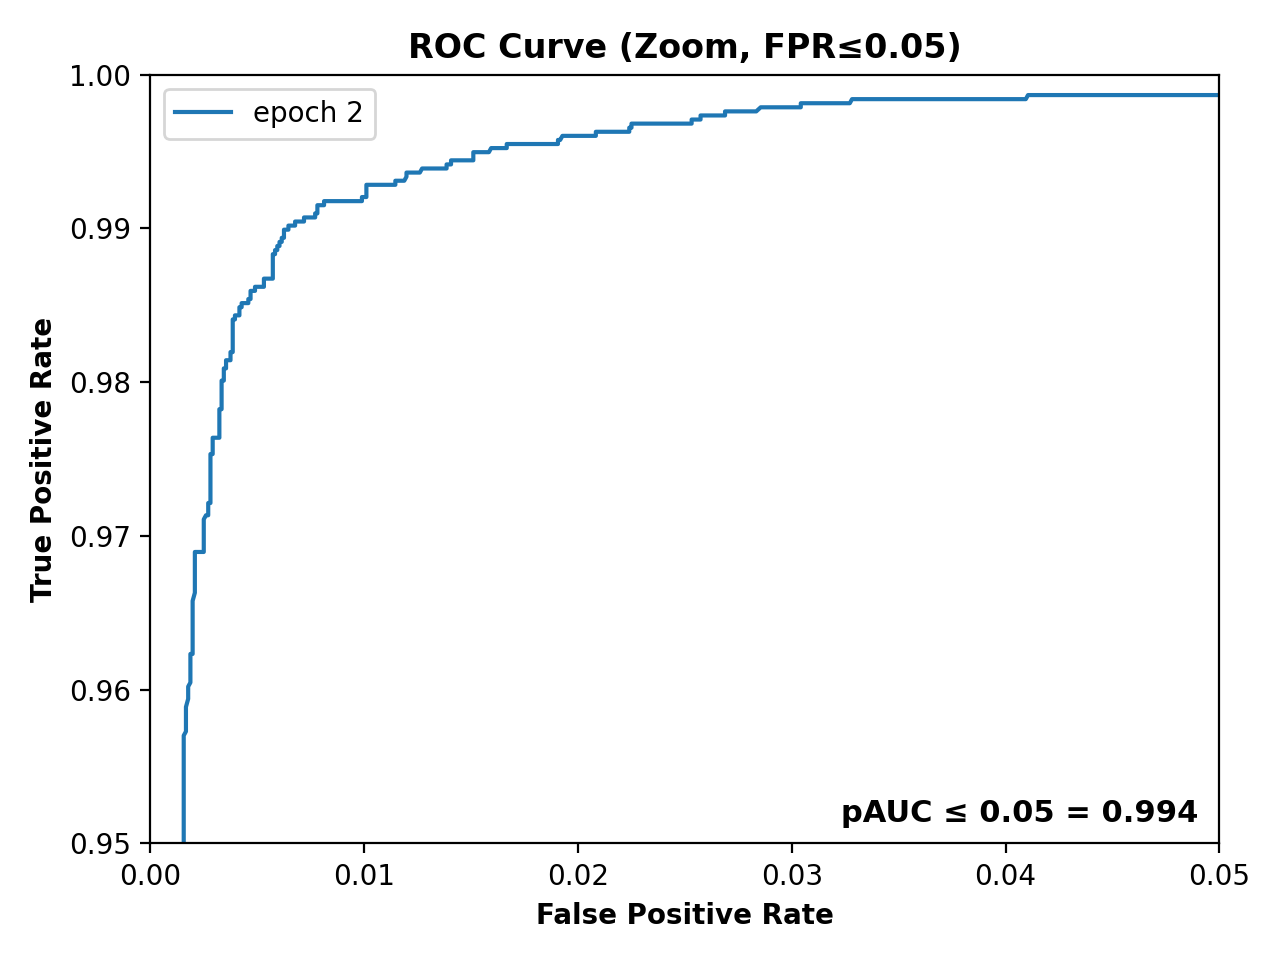
\includegraphics[width=\linewidth]{plots_feature_fusion_subset/epoch_2_plots/roc_zoom_epoch_2.png}
    \caption{Epoch 2}
    \label{fig:ffroc_all_e2}
  \end{subfigure}\hfill
  \begin{subfigure}[t]{0.32\textwidth}
    \centering
    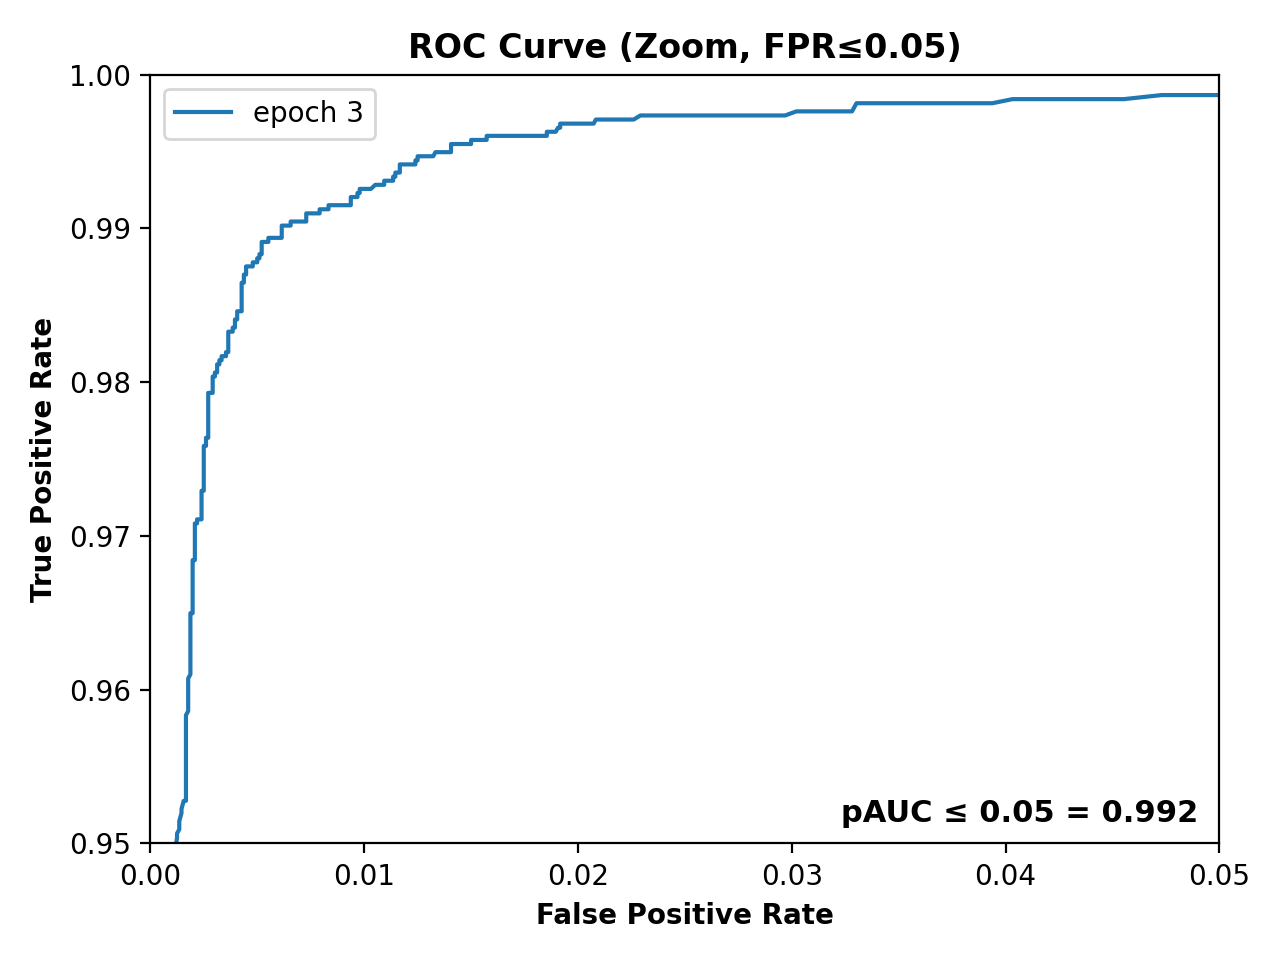
\includegraphics[width=\linewidth]{plots_feature_fusion_subset/epoch_3_plots/roc_zoom_epoch_3.png}
    \caption{Epoch 3}
    \label{fig:ffroc_all_e3}
  \end{subfigure}


  \caption[Zoomed ROC curves for feature-fusion models across epochs.]{\textbf{Zoomed ROC curves for feature-fusion models across all three epochs.}
  \emph{Top row:} fusion with all LIWC-2022 features. \emph{Bottom row:} fusion with the psychometric LIWC-2022 subset.
  Columns show epochs 1–3. All panels display the same zoom window to highlight differences at low false-positive rates
  (\(\mathrm{FPR}\le 0.05,\ \mathrm{TPR}\ge 0.95\)); the legend in each plot reports the pAUC of the \emph{full} ROC curve.}
  \label{fig:ff_roc_zoom_epochs}
\end{figure}

Figure \ref{fig:ff_roc_zoom_epochs} shows the zoomed ROC curves for both feature-fusion configurations across three epochs. It is notable that both configurations achieve very high pAUC values, indicating excellent overall discrimination between grooming and non-grooming conversations. Also, the curves for both configurations are very steep at a very low false positive rate, indicating that the models can achieve high true positive rates while keeping false positives very low. Especially in epoch 1, there is a light difference between the two configurations, with the model using all LIWC-2022 features showing a slightly better performance. However, as training progresses to epochs 2 and 3, the differences between the two configurations become negligible, with both achieving nearly identical, almost perfect performance in epoch 3. Consequently, the zoomed-in view reveals that both models maintain high true positive rates even at very low false positive rates, across all three epochs of training and for both configurations (all LIWC-Features and only psychometric subset of features). This suggests that the feature-fusion balances sensitivity and specificity effectively. Also, the pAUC lies between 0.987 and 0.994, showing stable performance across all epochs and configurations.

When comparing the ROC curves of the feature-fusion models to the BERT baseline in figure \ref{fig:roc_zoom_epoch3}, it is evident that the fusion models achieve a  better performance, particularly at very low false positive rates for both configurations with more stable and steep ROC-Curves. This is also true when using only a subset of psychometric LIWC-Features, indicating that the addition of LIWC features helps the model maintain high sensitivity while reducing false positives as already shown in the confusion matrices at Figure \ref{fig:ff_confmats_epochs}. However, the differences are relatively small since the differences are only visible at a very small FPR, suggesting that while LIWC features provide additional value, the BERT embeddings already capture much of the relevant information. \textbf{Overall, the ROC analysis confirms that feature fusion enhances model robustness and reliability in detecting grooming behavior, particularly in scenarios where minimizing false positives is critical.} 

\section{Ablation Studies based on SHAP} \label{sec:ablation_studies_shap}

The results of the ablation studies based on SHAP are presented in the following sections. The analysis focuses on understanding the contribution of individual LIWC features to the model's predictions and identifying the most influential features for distinguishing between grooming and non-grooming conversations. The results of the SHAP Analysis were once computed for only the "real" data (PJ + PAN12) to show their how they can be distinguished based on LIWC-Features and once for the complete dataset (PJ + PAN12 + synthetic) to show how the synthetic data influences the feature importance since the synthetic data was used during training to improve model robustness.

\subsection{LIWC-Feature Importance Ranking} 

To show there results of the LIWC-based SHAP Analysis, several steps were taken. First, the cumulative curves of all features were plotted to show how many features are needed to explain a certain percentage of the model decision (Figure \ref{fig:cumulative_feature_importance_combined}). Next, a global ranking of the top 20 features was created based on their percentages of the total significance (Figure \ref{fig:global_feature_importance_combined}). The results were then evaluated by class and visualized according to the direction of the effect (Figure \ref{fig:feature_importance_by_class_combined}). This makes it possible to understand which LIWC features are particularly relevant and whether they shift the model prediction toward grooming or non-grooming.


\subsubsection{Cumulative Feature Importance}

To gain a better understanding of the cumulative importance of features, the cumulative feature importance plots for all the used LIWC-Features were created. These plots show how many features are needed to explain a certain percentage of the model decision.

\begin{figure}[H]
  \centering
  
  % Erste Reihe: mit synthetischen Daten
  \begin{subfigure}[t]{0.49\textwidth}
    \centering
    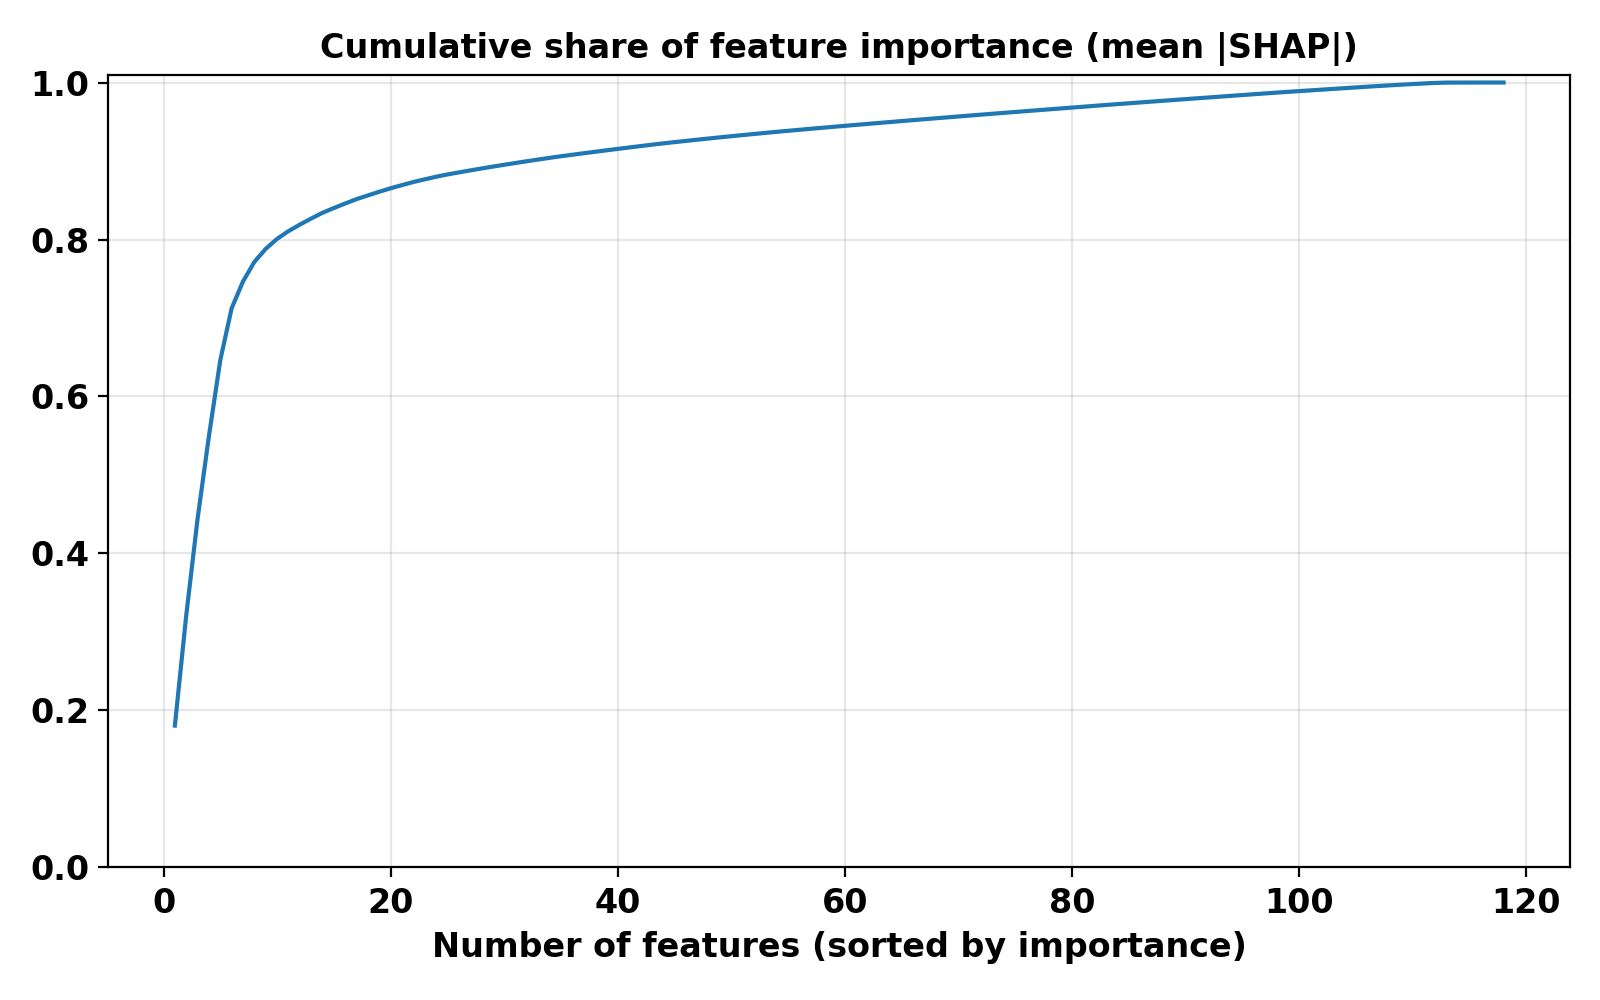
\includegraphics[width=\linewidth,height=6cm,keepaspectratio]{cumulative_importance_synth.png}
    \caption{All LIWC-2022 features (with synthetic data).}
    \label{fig:cum_synth_all}
  \end{subfigure}\hfill
  \begin{subfigure}[t]{0.49\textwidth}
    \centering
    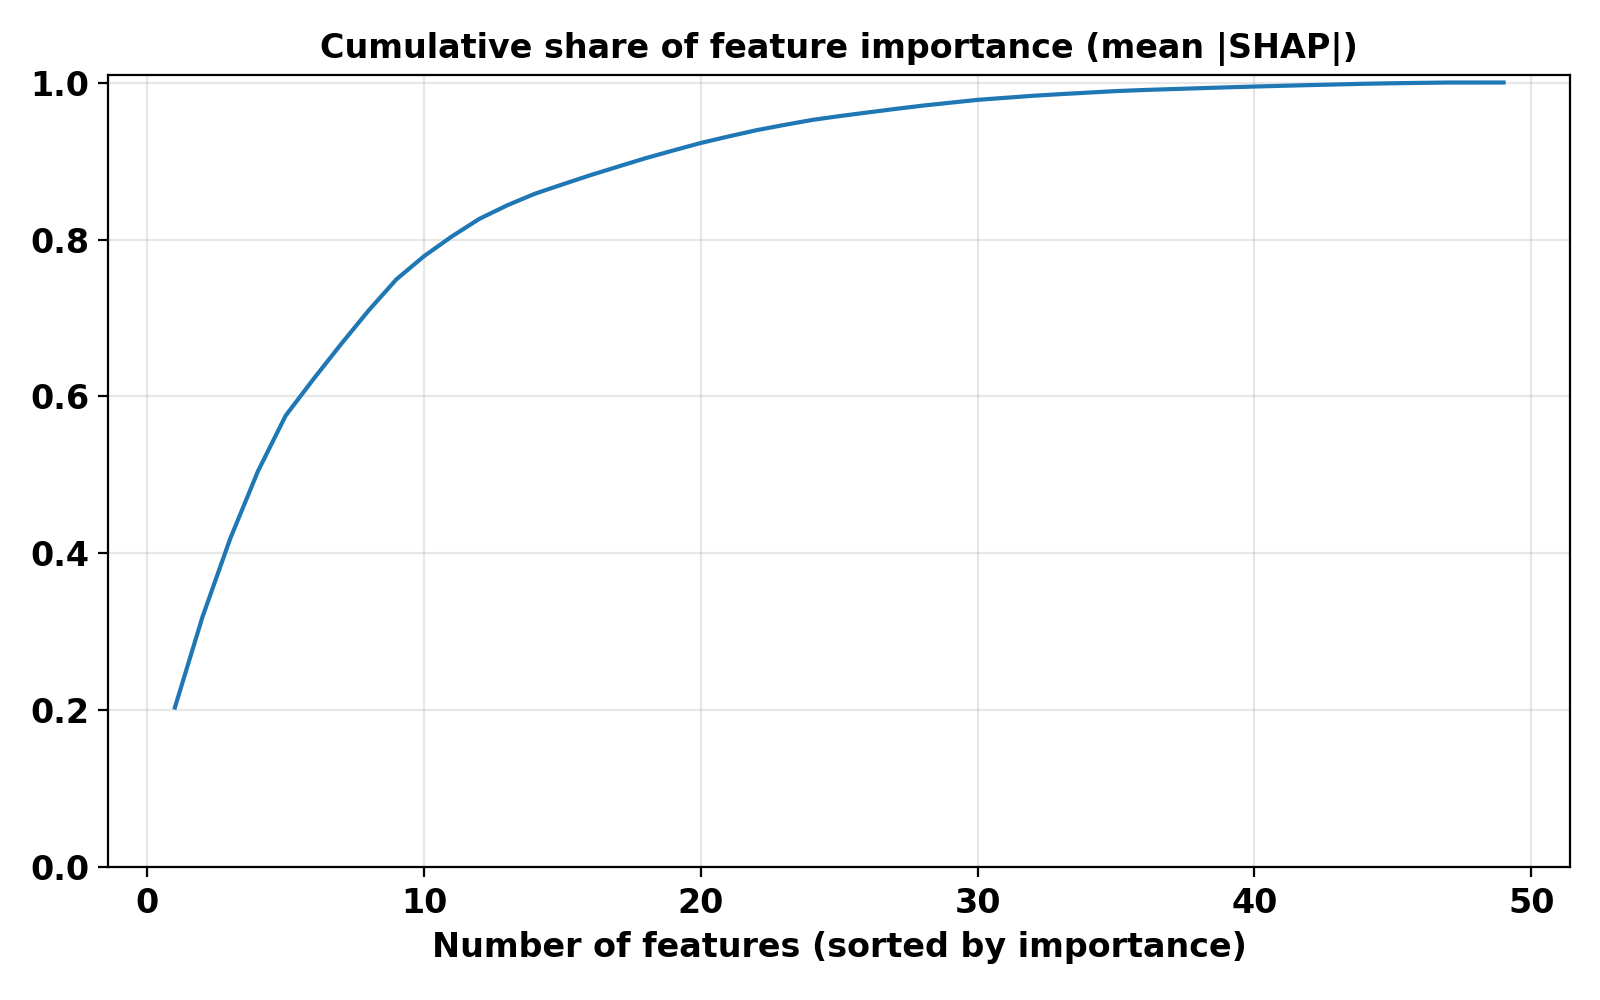
\includegraphics[width=\linewidth,height=6cm,keepaspectratio]{cumulative_importance_psycho_synth.png}
    \caption{Psychometric subset (with synthetic data).}
    \label{fig:cum_synth_psycho}
  \end{subfigure}
  
  \vspace{0.5cm}
  
  % Zweite Reihe: ohne synthetische Daten
  \begin{subfigure}[t]{0.49\textwidth}
    \centering
    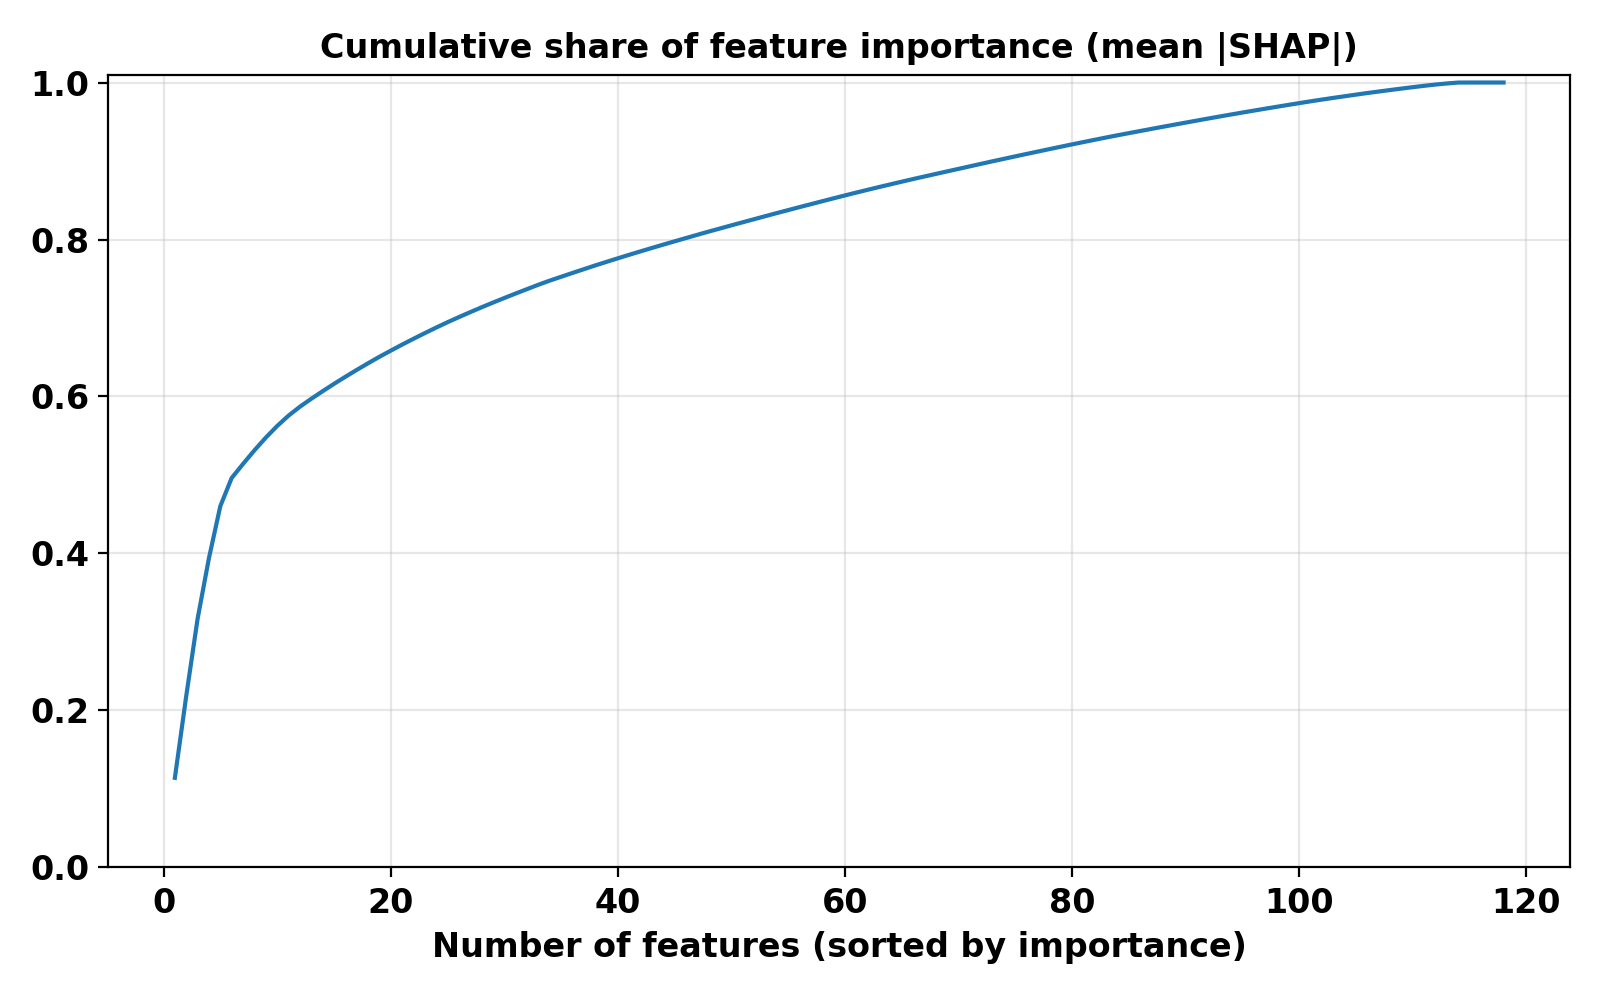
\includegraphics[width=\linewidth,height=6cm,keepaspectratio]{cumulative_importance_all_no_synth.png}
    \caption{All LIWC-2022 features (no synthetic data).}
    \label{fig:cum_no_synth_all}
  \end{subfigure}\hfill
  \begin{subfigure}[t]{0.49\textwidth}
    \centering
    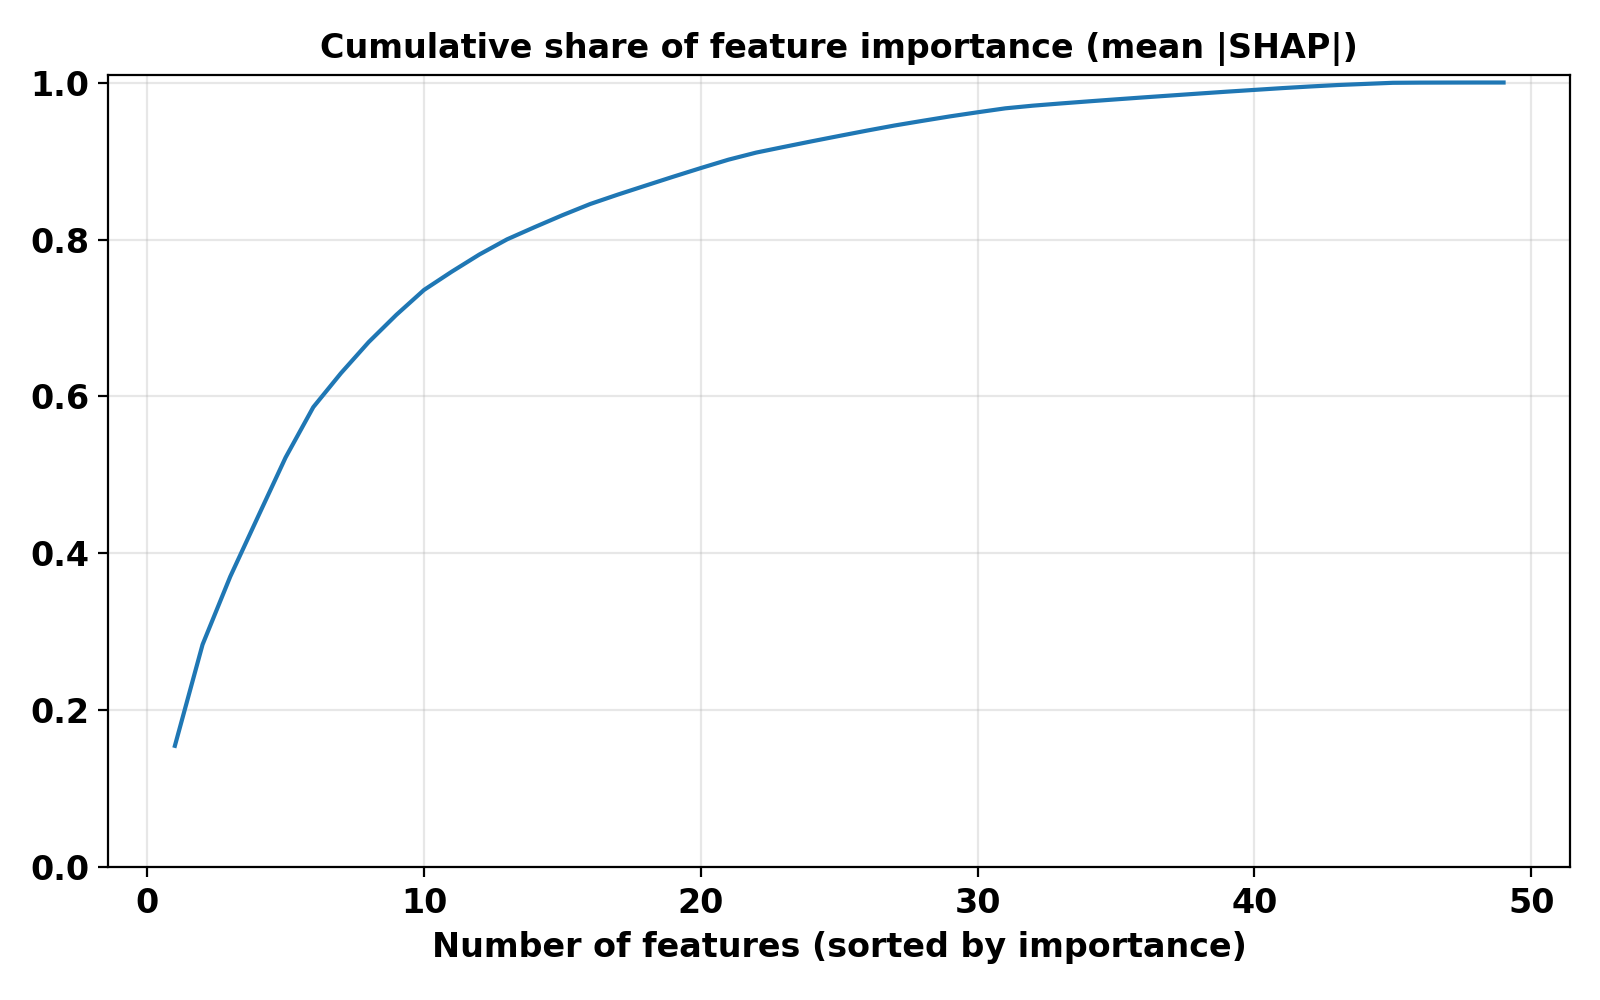
\includegraphics[width=\linewidth,height=6cm,keepaspectratio]{cumulative_importance_psycho_no_synth.png}
    \caption{Psychometric subset (no synthetic data).}
    \label{fig:cum_no_synth_psycho}
  \end{subfigure}

  \caption[Cumulative importance of LIWC-2022 features.]{\textbf{Cumulative importance of LIWC-2022 features.} 
  Top row: with synthetic data. Bottom row: no synthetic data.}
  \label{fig:cumulative_feature_importance_combined}
\end{figure}

When looking at the curves of the cumulative feature importance (Figure \ref{fig:cumulative_feature_importance_combined}), especially on the psychometric subset with no synthetic data, it is noticeable that the top 10 features already explain about 80\% of the model decision and the top 20 features explain almost 100\%. This indicates that the model relies strongly on a few key features to make its predictions when only real data is used. Furthermore, when looking at the cumulative share at the psychometric subset including synthetic data, the top 10 features explain only about 60\% of the model decision, showing that the synthetic data leads to a more even distribution of feature importance across all features, which can be interpreted as a more robust model that does not rely too heavily on individual features. Still, the top 20 features explain almost 80\% of the model decision, indicating the reliance of the model on less than a half of the used psychometric features.

\textbf{Note, that the smaller size of the psychometric subset feature size leads in an overall higher importance per feature compared to the full feature set, where the importance is distributed over a larger number of features.} In comparison to the curves based on the psychometric subset, the curves based on all LIWC-2022 features show a more gradual increase, indicating that the model relies on a broader range of features to make its predictions. This is particularly evident when synthetic data is included, where the top 20 features explain only about 40\% of the model decision and the top 40 features explain about 60\%. In contrast, when no synthetic data is included, the top 20 features explain about 50\% of the model decision and the top 40 features explain about 70\% which is still a significant portion regarding the total amount of 118 features.This suggests that the inclusion of synthetic data encourages the model to consider a wider array of features, potentially leading to improved generalization and robustness. Also, it is noticeable that the last 20 feature with the least importance in the full feature set explain only about 5\% of the model decision, indicating that these features contribute very little to the model's predictions and could potentially be excluded without significantly impacting the model performance.

To gain a deeper understanding of which specific LIWC features are the most influential in the model's decision-making process, a global ranking of the top 20 features was created based on their percentages of the total significance since the top 20 features hold the majority of the model's importance for both fusion configurations. The results are presented in the following Figure \ref{fig:global_feature_importance_combined}.


\begin{figure}[H]
  \centering
  
  % Erste Reihe: mit synthetischen Daten
  \begin{subfigure}[t]{0.49\textwidth}
    \centering
    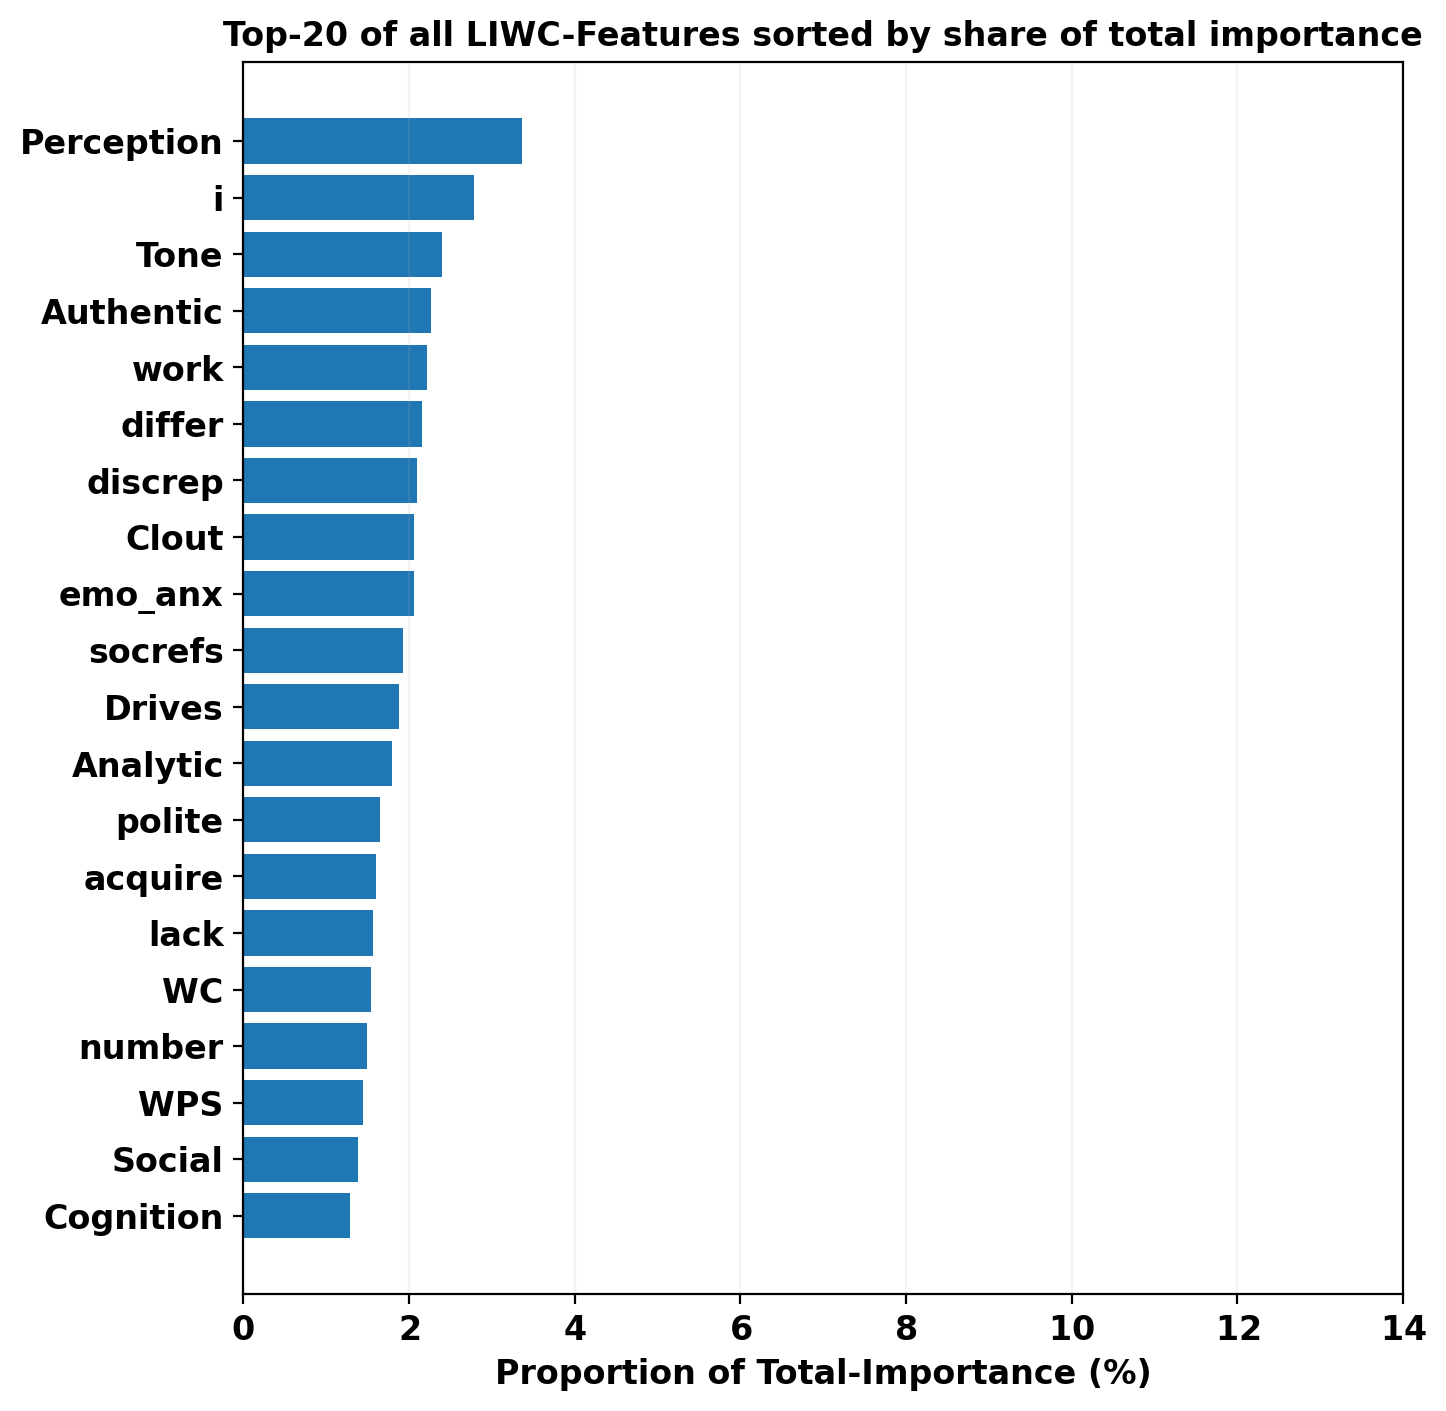
\includegraphics[width=\linewidth,height=6cm,keepaspectratio]{topN_share_importance_synth.png}
    \caption{All LIWC-2022 features (with synthetic data).}
    \label{fig:synth_all}
  \end{subfigure}\hfill
  \begin{subfigure}[t]{0.49\textwidth}
    \centering
    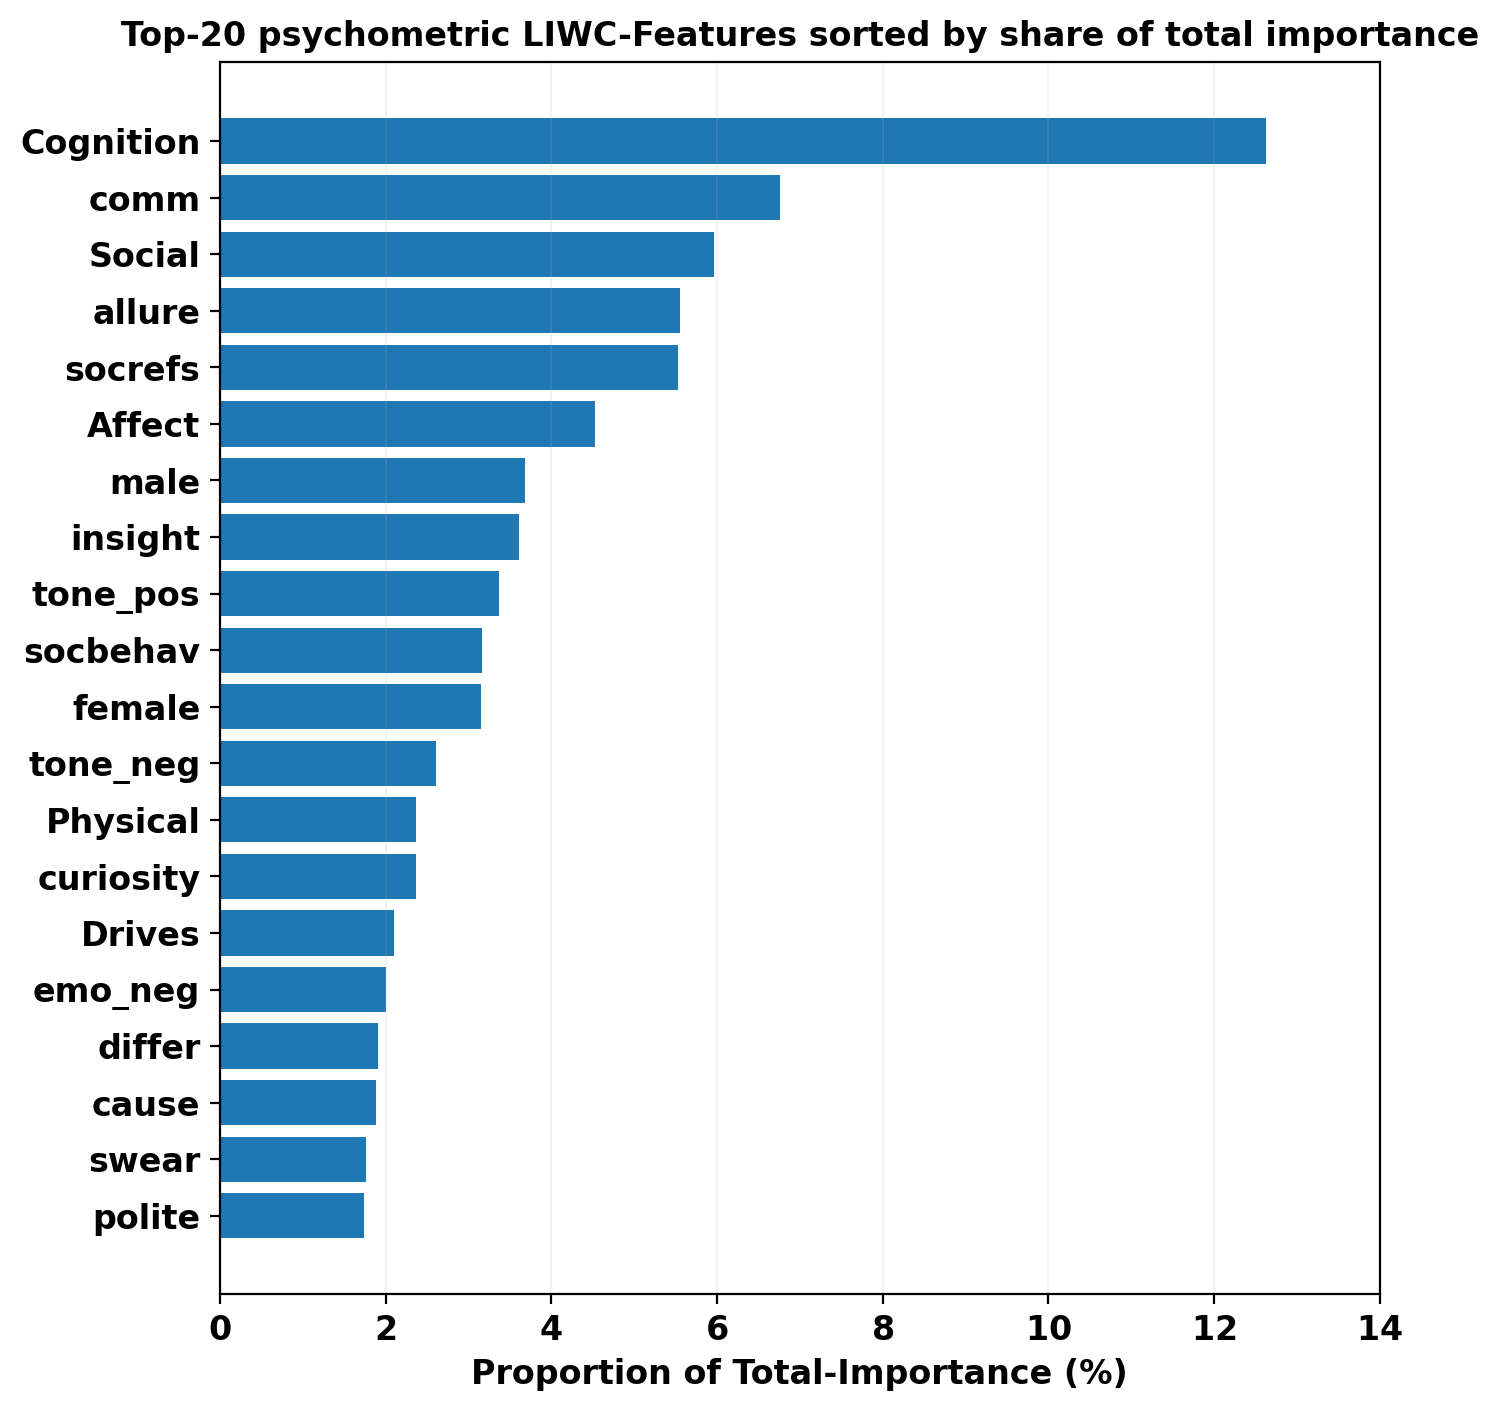
\includegraphics[width=\linewidth,height=6cm,keepaspectratio]{topN_share_importance_psycho_synth.png}
    \caption{Psychometric subset (with synthetic data).}
    \label{fig:synth_psycho}
  \end{subfigure}
  
  \vspace{0.5cm}
  

  \begin{subfigure}[t]{0.49\textwidth}
    \centering
    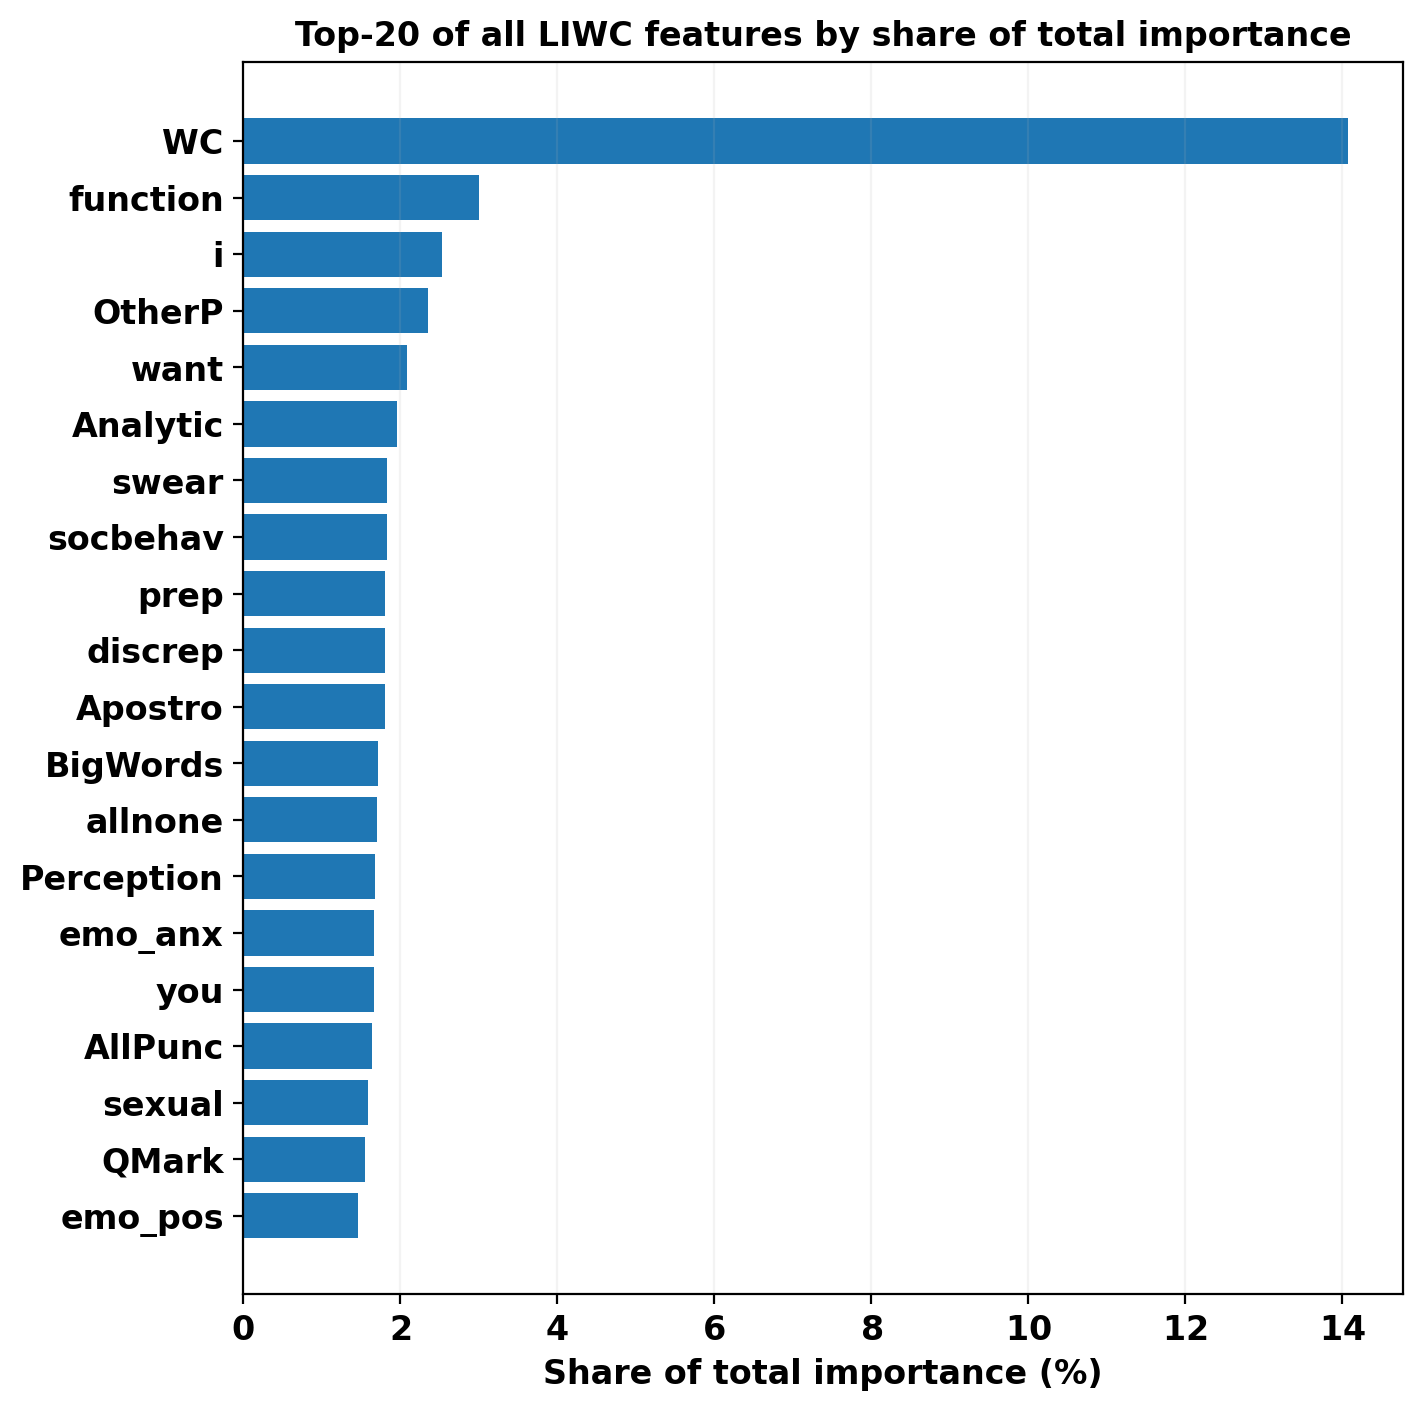
\includegraphics[width=\linewidth,height=6cm,keepaspectratio]{topN_share_importance_no_synth.png}
    \caption{All LIWC-2022 features (no synthetic data).}
    \label{fig:no_synth_all}
  \end{subfigure}\hfill
  \begin{subfigure}[t]{0.49\textwidth}
    \centering
    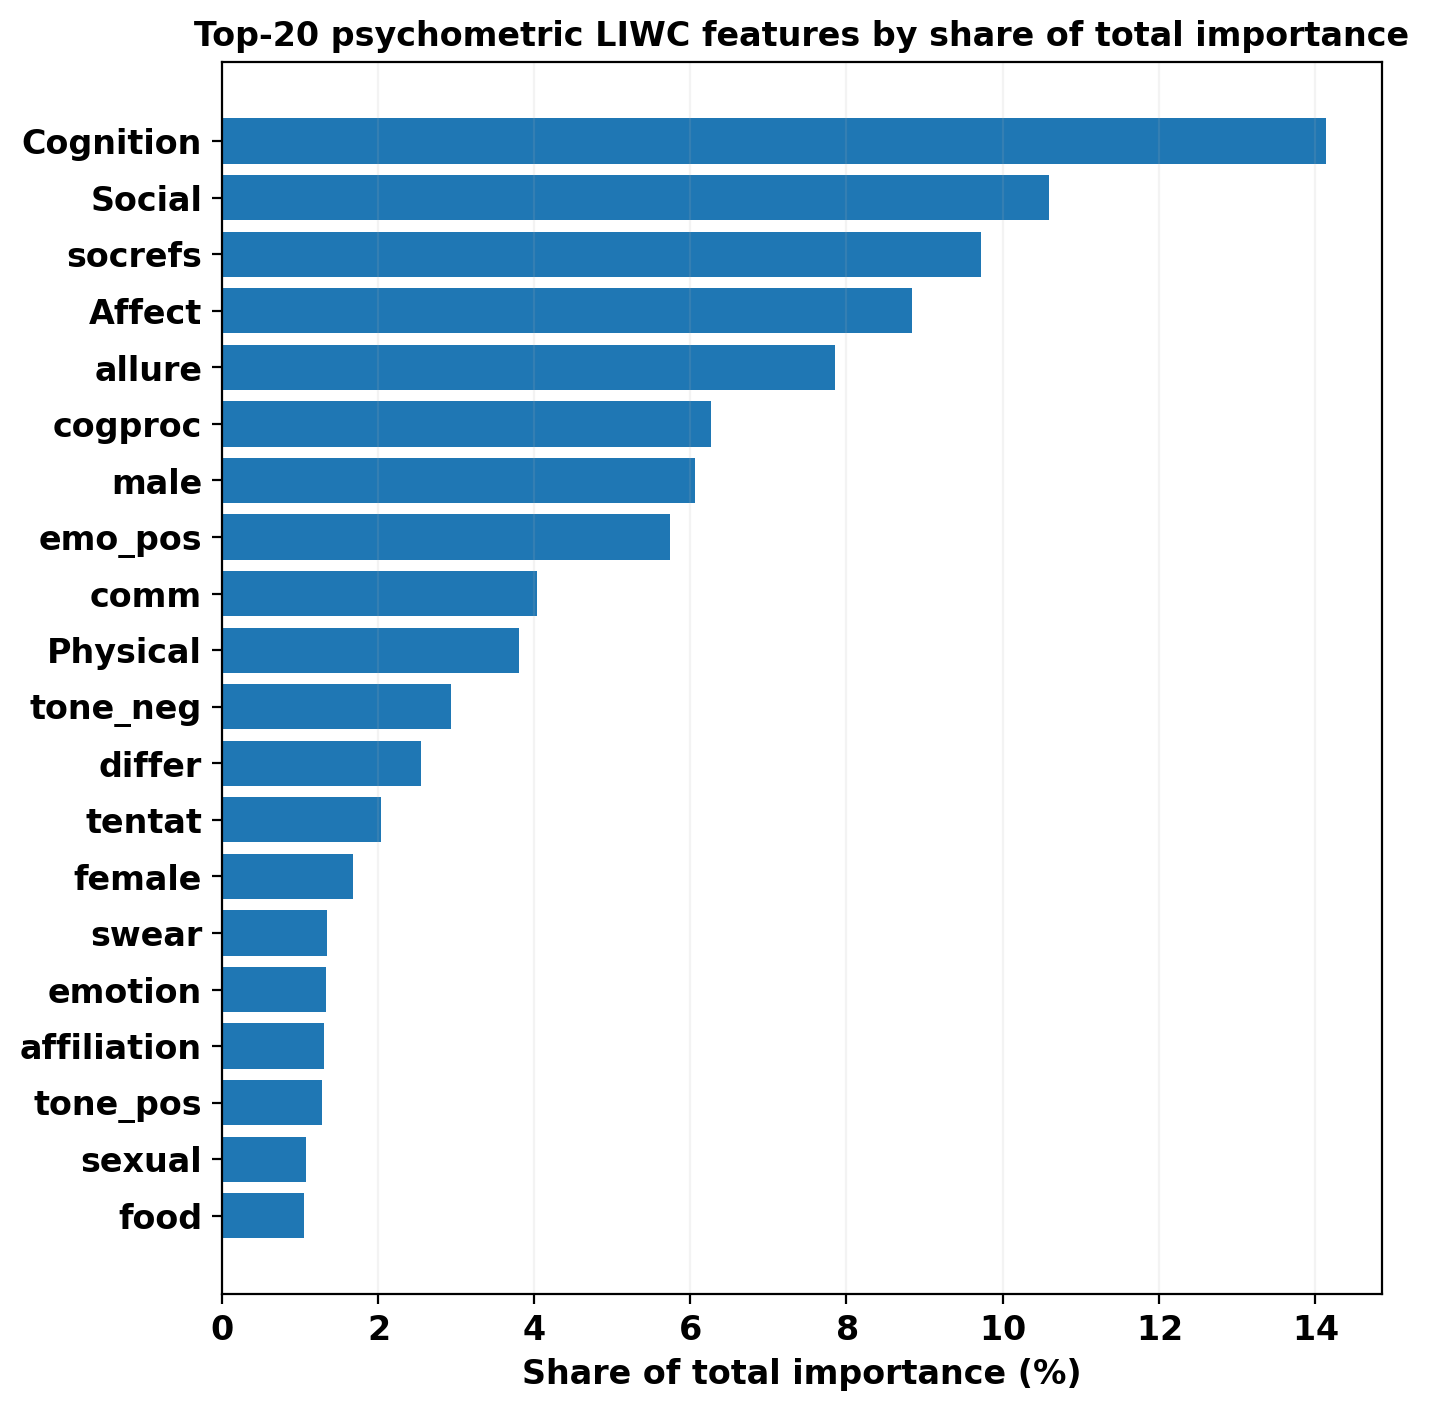
\includegraphics[width=\linewidth,height=6cm,keepaspectratio]{topN_share_importance_psycho_no_synth.png}
    \caption{Psychometric subset (no synthetic data).}
    \label{fig:no_synth_psycho}
  \end{subfigure}

  \caption[Top 20 LIWC features ranked by percentages of the total significance.]{\textbf{Top 20 LIWC features ranked by percentages of the total significance.} 
  Top row: with synthetic data. Bottom row: no synthetic data.}
  \label{fig:global_feature_importance_combined}
\end{figure}

The global rankings of the top 20 features (Figure~\ref{fig:global_feature_importance_combined}) confirm the observations from the cumulative curves. A comparatively small core of features contributes most to the model decision, with the type of features used differing between the full LIWC set and the psychometric subset, as well as between training with and without synthetic data.

\paragraph{All LIWC features (with synthetic data).}
\textbf{What is striking is a stronger weighting of \emph{content/psychological} categories like:} \textit{Perception}, \textit{i}, \textit{Tone}, \textit{Authentic}, \textit{Analytic}, \textit{Social}/\textit{Cognition} and relationship and status markers such as \textit{Clout} and \textit{polite}. Formal variables such as \textit{WC}, \textit{WPS} and \textit{number} also appear in the top 20, but are significantly less pronounced. \textbf{This suggests that synthetic data demonstrably reduces dependence on pure length signals and thus emphasizes semantic-psychological signals more}.

Note that, as already shown in the cumulative curves, the percentage feature importance per feature is generally lower for all LIWC-Features than in the psychometric subset. As already mentioned, this is probably explained by the generally larger feature set, which distributes the importance over a larger number of features that the model can rely on.

\paragraph{All LIWC features (without synthetic data).}
However, without synthetic data, \emph{formal} features dominate: \textit{WC} clearly ranks at the top, followed by \textit{function}, pronouns (\textit{i}, \textit{you}, \textit{OtherP}) and punctuation and word form features (\textit{AllPunc}, \textit{QMark}, \textit{Apostro}, \textit{BigWords}). Psychological categories (\textit{Analytic}, \textit{Perception}, \textit{emo\_anx}, \textit{sexual}) are present, but are clearly overshadowed by style and length indicators.
 

\paragraph{Psychometric subset (with synthetic data).}
Here, the focus is clearly on cognitive, social and affective processes such as Cognition (dominant), Social including socrefs/socbehav, Affect, \textit{allure}, \textit{comm}, \textit{insight}, \textit{tone\_pos}/\textit{tone\_neg} and \textit{Drives}. Gender markers (\textit{male}/\textit{female}) and \textit{Physical} appear as contextual signals. The distribution is more balanced than without synthetic data.


\paragraph{Psychometric subset (without synthetic data).}
The ranking remains stable at its core (\textit{Cognition}, \textit{Social}, \textit{Affect}, \textit{allure}), but the top is even more concentrated. In addition, thematic markers (\textit{sexual}, \textit{food}), uncertainty and deliberation signals (\textit{tentat}, \textit{differ}) and affiliation (\textit{affiliation}) are more prominent. This indicates that the model relies particularly heavily on fewer psychological features and more individual thematic cues in real data. Generally, it can be said, that the more even distribution of feature importance when using synthetic data suggests that the model is less dependent on individual features and thus more robust. Also, the importance of the features varies depending on the used configuration, which indicates that the model relies on different features to make its predictions. Still, in the psychometric subset, features like \textit{Cognition}, \textit{Social}, \textit{allure} and \textit{Affect} are consistently important across configurations, highlighting their relevance in distinguishing grooming from non-grooming conversations while in the full feature set, the importance of features varies more widely, indicating that the model may be leveraging a broader range of linguistic cues when all LIWC-2022 features are available.

To further gain insights into the direction of the effects of the individual features, the mean signed SHAP values were visualized in the following section.


\subsubsection{Singed Feature Importance by Class}

\begin{figure}[H]
  \centering
  
  % Erste Reihe: mit synthetischen Daten
  \begin{subfigure}[t]{0.49\textwidth}
    \centering
    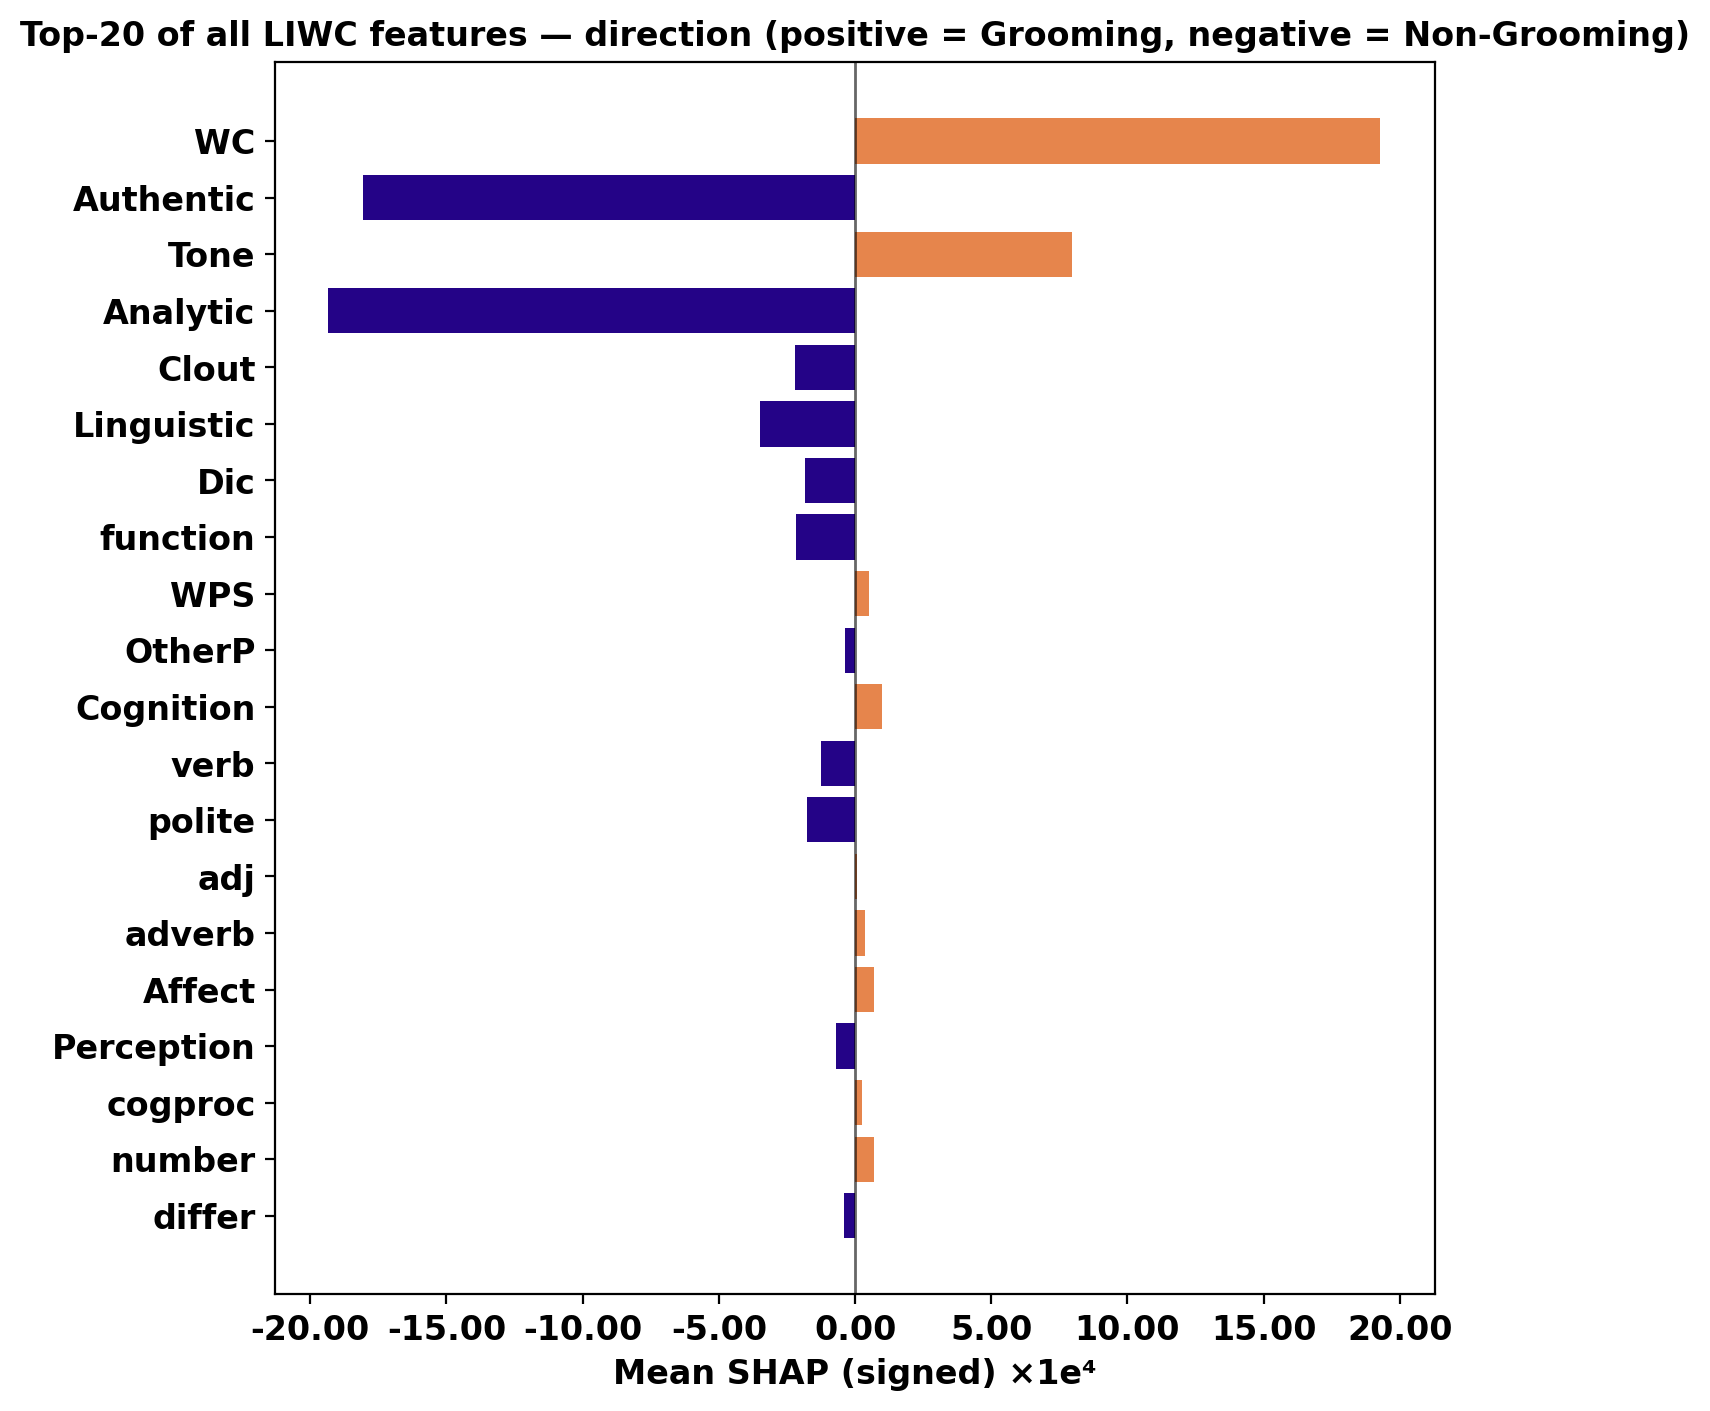
\includegraphics[width=\linewidth,height=6cm,keepaspectratio]{topN_mean_signed_importance_synth.png}
    \caption{All LIWC-2022 features (with synthetic data).}
    \label{fig:synth_all_shap}
  \end{subfigure}\hfill
  \begin{subfigure}[t]{0.49\textwidth}
    \centering
    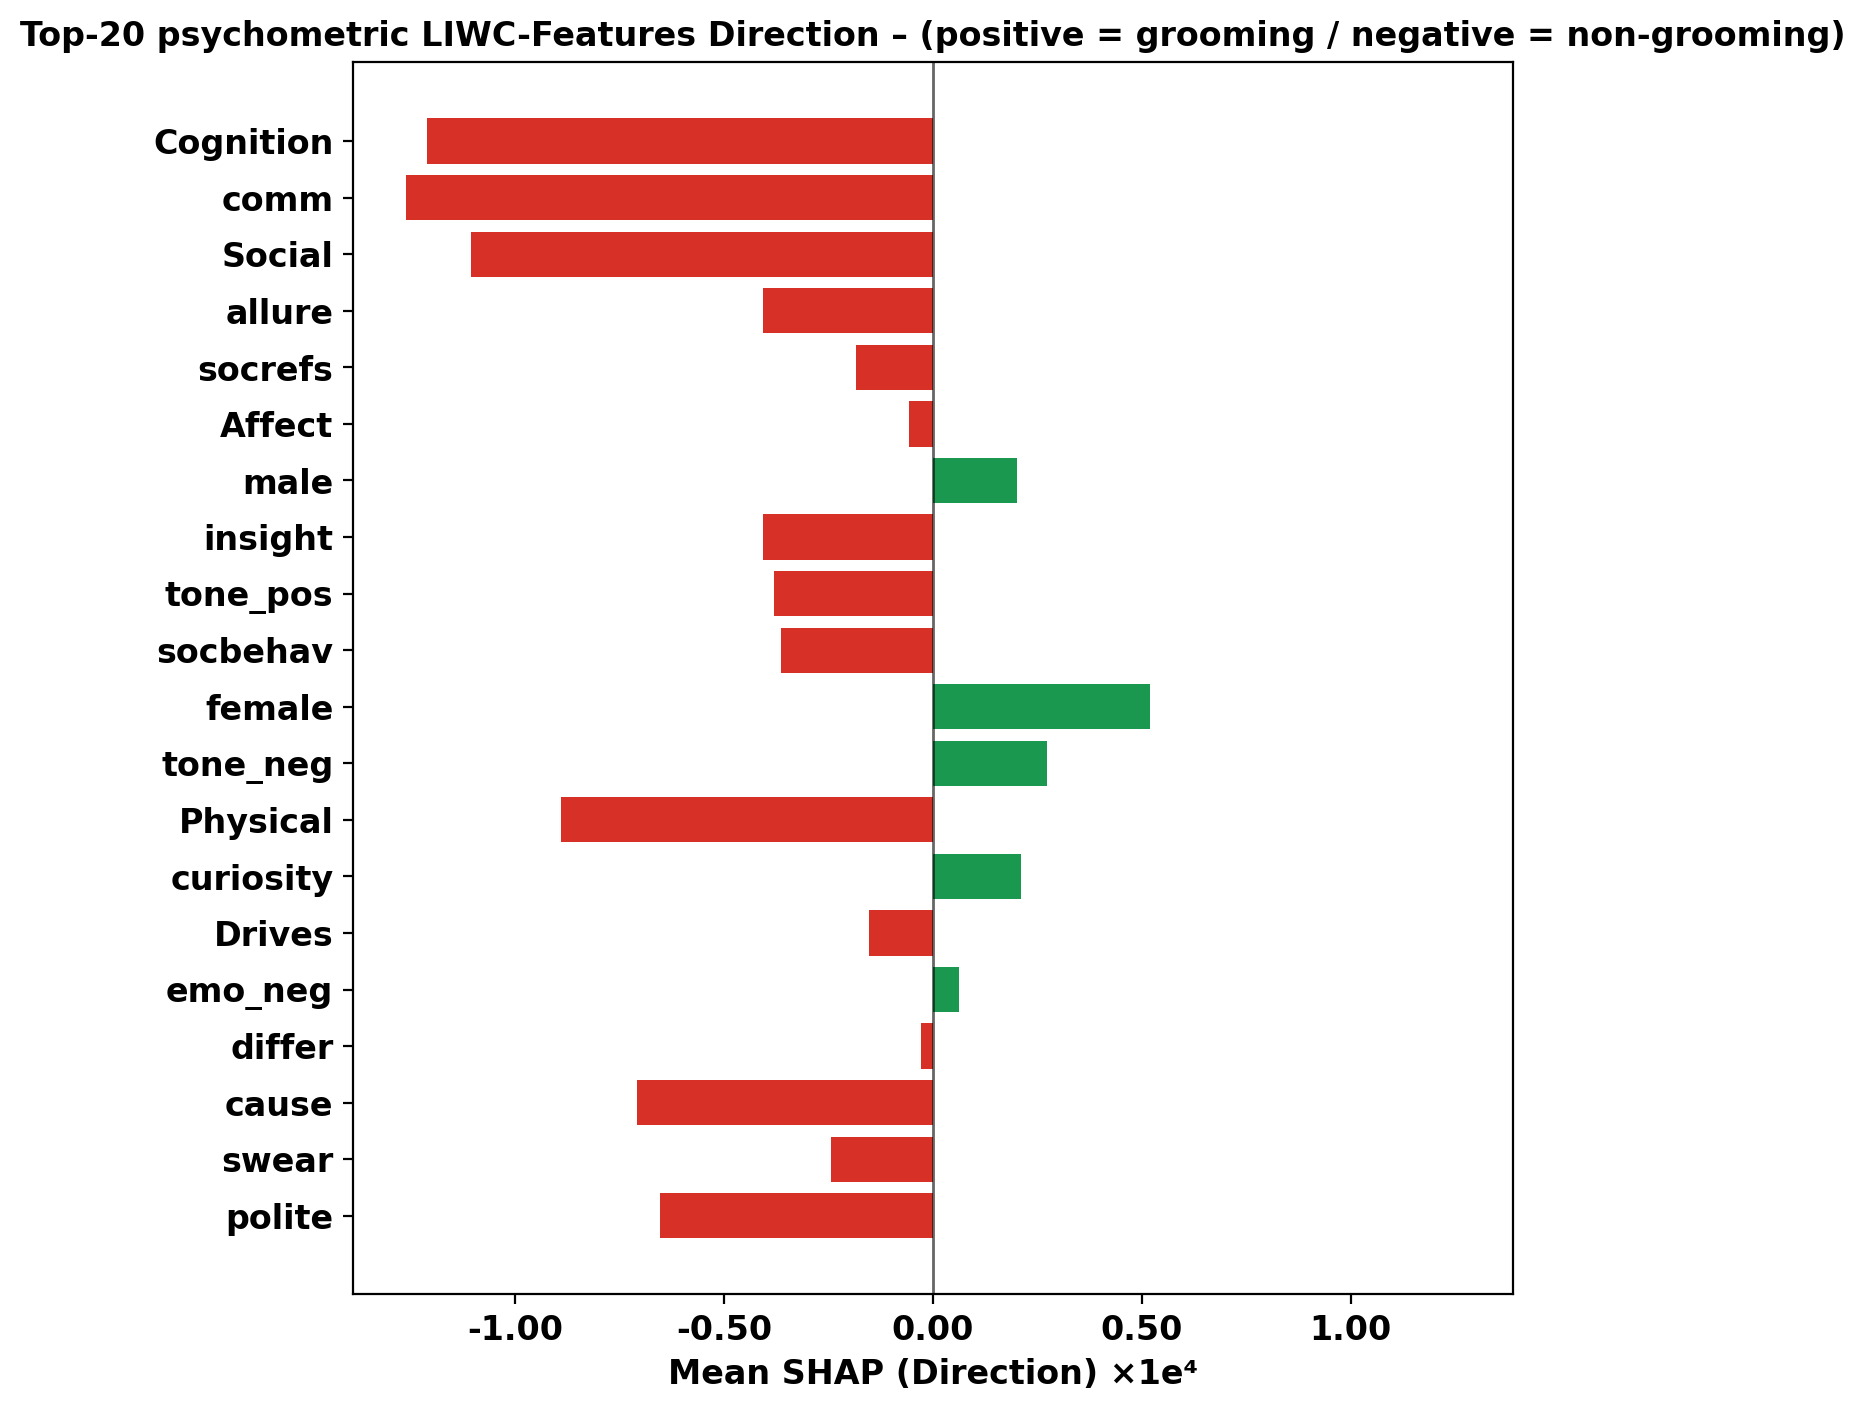
\includegraphics[width=\linewidth,height=6cm,keepaspectratio]{topN_mean_signed_importance_psycho_synth.png}
    \caption{Psychometric subset (with synthetic data).}
    \label{fig:synth_psycho_shap}
  \end{subfigure}
  
  \vspace{0.5cm}
  
  % Zweite Reihe: ohne synthetische Daten
  \begin{subfigure}[t]{0.49\textwidth}
    \centering
    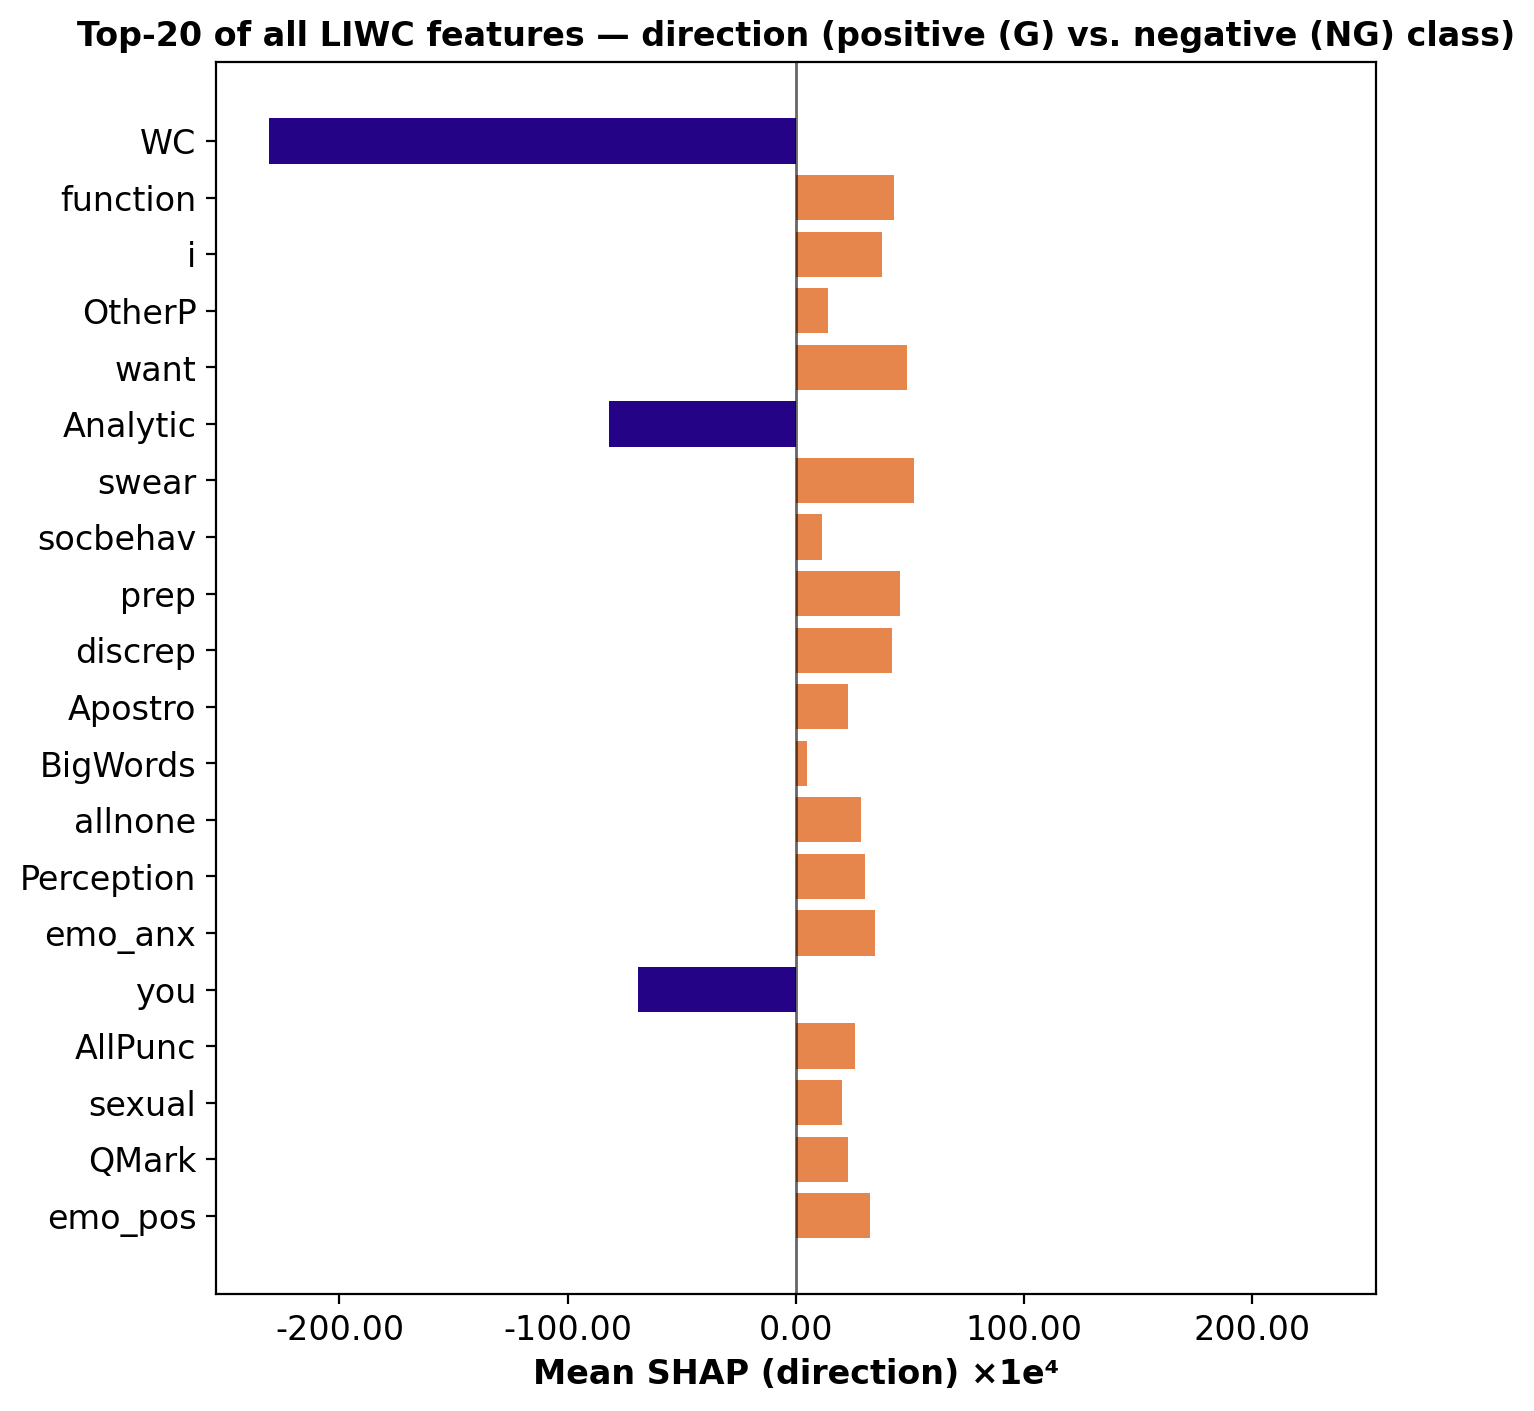
\includegraphics[width=\linewidth,height=6cm,keepaspectratio]{topN_mean_signed_importance_all_no_synth.png}
    \caption{All LIWC-2022 features (no synthetic data).}
    \label{fig:no_synth_all_shap}
  \end{subfigure}\hfill
  \begin{subfigure}[t]{0.49\textwidth}
    \centering
    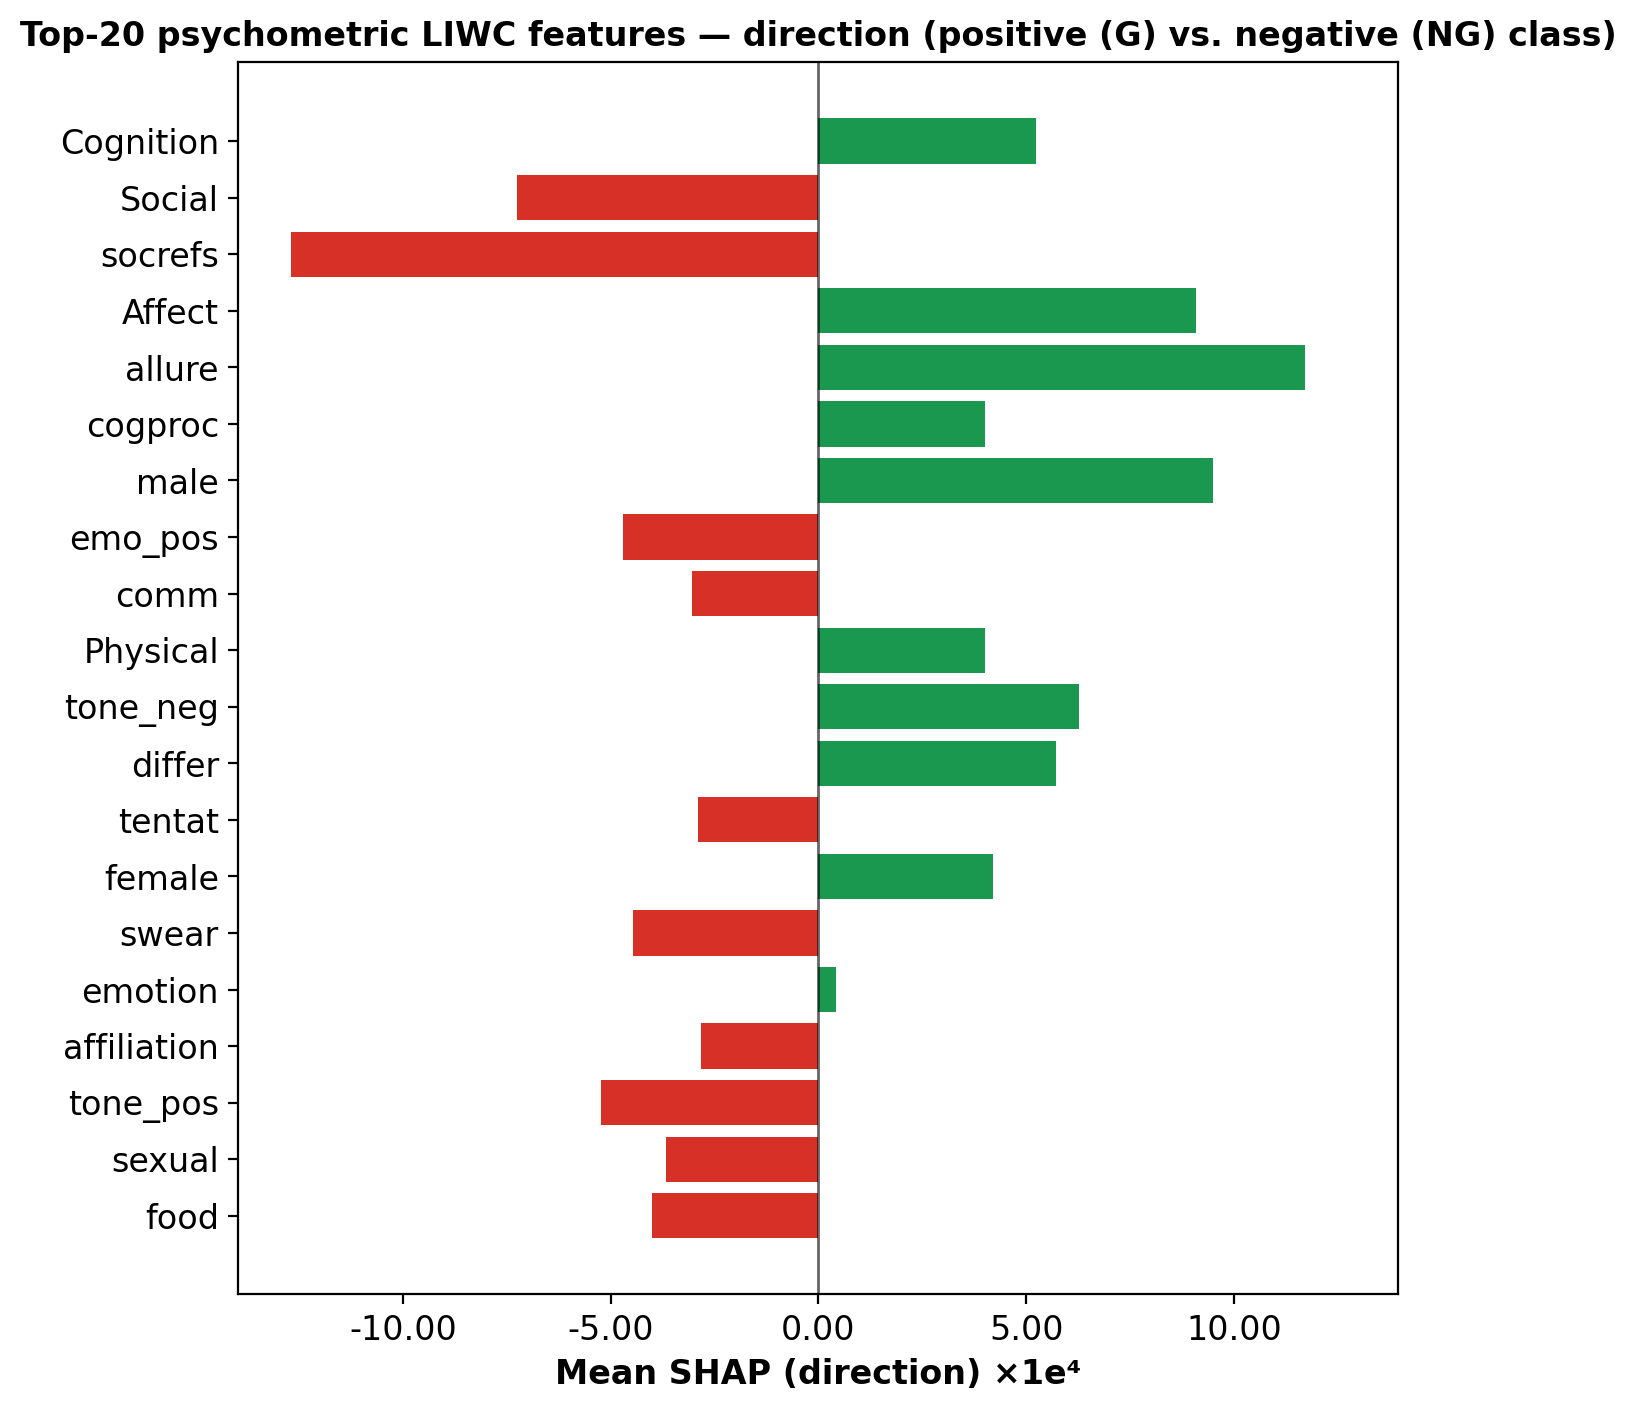
\includegraphics[width=\linewidth,height=6cm,keepaspectratio]{topN_mean_signed_importance_psycho_no_synth.png}
    \caption{Psychometric subset (no synthetic data).}
    \label{fig:no_synth_psycho_shap}
  \end{subfigure}

  \caption[Top 20 LIWC features ranked by mean signed SHAP value.]{\textbf{Top 20 LIWC features ranked by mean signed SHAP value.} 
  Top row: with synthetic data. Bottom row: no synthetic data. 
  Positive values indicate a shift toward the grooming class, negative values toward the non-grooming class. 
  \textit{Note: the scales differ between the plots. The left-hand plots (all features) have a larger range than the right-hand plots (psychometric subset).}}
  \label{fig:feature_importance_by_class_combined}
\end{figure}

Figure \ref{fig:feature_importance_by_class_combined} shows the top 20 LIWC features ranked by their mean signed SHAP values for both configurations (all LIWC-2022 features and psychometric subset) with and without synthetic data. Note, that the mean signed Feature plots show the same features as the global importance plots, but now colored by their direction of effect. Positive values indicate a shift toward the grooming class, negative values toward the non-grooming class. 

\paragraph{Note on axis scaling (effect magnitudes).}
The x-axis (mean \emph{signed} SHAP value) is scaled very differently across panels. In particular, \emph{All LIWC-2022 features (with synthetic data)} spans roughly $[-200,+200]\times 10^{4}$, whereas \emph{Psychometric subset (no synthetic data)} spans about $[-10,+10]\times 10^{4}$ and \emph{Psychometric subset (with synthetic data)} about $[-1,+1]\times 10^{4}$. 
Thus, absolute effects are \emph{much larger} in the "All LIWC + synthetic" panel, even when bars look visually similar, followed by the psychometric/no-synthetic panel and, lastly, the psychometric/with-synthetic panel. 
Consequently, bar lengths should be compared primarily \emph{within} a panel and not in between. For cross-panel comparisons, only focus on \emph{direction} (sign) and \emph{ranking}.

\paragraph{Interpretation of directional effects.}
Instead of listing individual features, Figure~\ref{fig:feature_importance_by_class_combined} reveals a pattern according to which dialogues are classified as grooming or non-grooming:
 
Language that is structured in a \emph{cognitive-reflexive and cooperative} manner (planning/explaining, referring to conversation partners, polite and predominantly positive tone) shifts the decision toward \textbf{non-grooming}. In contrast, \emph{emotionally charged, boundary-testing and closeness-creating} signals (negative/tense tone, heightened affect, uncertainty/consideration, targeted information gathering or “luring,” and explicit sexual references) indicate \textbf{grooming}. This picture complements the global and cumulative analyses of the previous sections. The content-related psychological processes drive the separation, while formal text features (length, punctuation) act as stronger indicators, especially without synthetic data.

\paragraph{All features with vs. without synthetic data}
With synthetic data, the \emph{semantic-psychological} contrast becomes clearly apparent. Here, cognitively and socially ordered and positive conversation tends to lean toward non-grooming, while tonal/affective tensions, authenticity/status signals and typical questioning movements (e.g., about age/contact) shift the decision toward grooming. Without synthetic data, however, the decision shifts more frequently toward non-grooming via \emph{formal proxies} such as text length or punctuation patterns, while grooming components are fed by many smaller, stylistic-affective cues. This shift toward formal characteristics explains the steeper, “sharper” cumulative importance without synthetic data and underscores the risk of more unnatural correlations.

\paragraph{Psychometric subset with vs. without synthetic data.}
In the psychometric space, the decision direction is particularly plausible.
\emph{Cognition/cooperation/positive tone} mark non-grooming, while \emph{negative affect, tone intensification, boundary tests/uncertainty and intimate context signals} mark grooming. With synthetic data, however, ambivalent categories (such as “compliments/allure” or vulgar language markers) are smoothed out and lose their one-sided grooming tendency. Without synthetic data, the profile becomes sharper and grooming and boundary testing patterns come to the fore. The cumulative curves \ref{fig:cumulative_feature_importance_combined} explain this difference. Synthetic data distributes importance more evenly and reduces the dominance of individual “sharp” indicators.

\textbf{ Note that the SHAP results indicate that several features change their direction when synthetic data are included, suggesting that the feature attribution is sensitive to the underlying data composition.} This is particularly evident in the psychometric subset, where top features like \textit{allure} and \textit{Cognition} shift the direction of their effect when synthetic data is included. This sensitivity highlights the importance of considering data composition when interpreting feature importance and suggests that the model's reliance on certain features may vary depending on the training data used.


\section{Confidence Analysis and Label Flip Analysis} \label{sec:confidence_and_label_flip_analysis}

In addition to the performance metrics and feature importance analysis, further evaluations were conducted to analyze the model's confidence in its predictions and to analyze instances where the model's predictions changed between evaluations after using LIWC-Features als additional model Inputs. This analysis was conducted on the dataset including synthetic data to assess the overall behavior of the model with and without LIWC features. \textbf{For the analysis, a total of 6849 samples were evaluated to reduce computational effort.}

\begin{figure}[H]
  \centering
  
  % All features
  \begin{subfigure}[t]{0.49\textwidth}
    \centering
    \includegraphics[width=\linewidth,height=6cm,keepaspectratio]{confidence_analysis_plots/maxprob_scatter.png}
    \caption{Confidence shift analysis for all LIWC-2022 features.}
    \label{fig:confshift_all}
  \end{subfigure}\hfill
  % Psychometric subset
  \begin{subfigure}[t]{0.49\textwidth}
    \centering
    \includegraphics[width=\linewidth,height=6cm,keepaspectratio]{confidence_analysis_psycho_plots/maxprob_scatter.png}
    \caption{Confidence shift analysis for psychometric LIWC-2022 subset.}
    \label{fig:confshift_psycho}
  \end{subfigure}

  \caption[Confidence shift analysis with LIWC features.]{\textbf{Confidence shift analysis with LIWC features.} 
  Left: all LIWC-2022 features. Right: psychometric subset of LIWC-2022 features. 
  Both plots show model confidence with LIWC set to zero (x-axis) versus LIWC as-is (y-axis). 
  The diagonal indicates no effect. 
  Points above the diagonal correspond to increased confidence due to LIWC features, while points below indicate reduced confidence. 
  The farther a point lies from the diagonal, the stronger the influence of LIWC features on model confidence. }
  \label{fig:confidence_shift}

\end{figure}


When looking on figure \ref{fig:confidence_shift} it can been seen that for all LIWC-2022 features (left), a lot of samples lie above the diagonal, indicating that the model's confidence in its predictions increased when LIWC features were included. Also, most of the samples lie close to the upper border (0.9 - 1.0) indicating an overall really high confidence of the model in its predictions using all LIWC-2022 features.
This suggests that the additional information provided by the full LIWC feature set helps the model make more confident predictions in most of the cases. Note that there are also some points underneath the diagonal showing that in some cases the model confidence decreased when LIWC features were included. 

When looking on the psychometric subset of LIWC-2022 features (right), a similar pattern can be observed, but the effect is less pronounced. While there are still many points above the diagonal indicating increased confidence, the points are more widely spread and lie closer to the diagonal, suggesting that the impact of the psychometric subset on model confidence is more moderate compared to using all LIWC features. This indicates that while the psychometric features are still valuable, they may not provide as much additional information as the full feature set.

The following table \ref{tab:confidence_label_flip} additionally shows the results of the confidence and label flip analysis for both the complete LIWC-2022 feature set and the psychometric subset after analyzing 6849 samples.

\begin{table}[H]
\centering
\caption{Confidence and label flip analysis for all LIWC-2022 features vs. psychometric subset.}
\begin{tabular}{lcc}
\toprule
\textbf{Metric} & \textbf{All Features} & \textbf{Psychometric Subset} \\
\midrule
Number of samples ($n$)            & 6849    & 6849 \\
$\Delta \mu$ (mean)                & 0.1543  & 0.0219 \\
$\Delta \tilde{x}$ (median)        & 0.2363  & 0.0313 \\
$\Delta \sigma$ (std)              & 0.1481  & 0.0256 \\
$\Delta p_{10}$                    & -0.0166 & -0.0020 \\
$\Delta p_{90}$                    & 0.3081  & 0.0454 \\
Class 0 count                      & 4055    & 3942 \\
Class 1 count                      & 2794    & 2907 \\
Flipped predictions                & 156     & 9 \\
Flip rate                          & 0.0228  & 0.0013 \\
\bottomrule
\end{tabular}
\label{tab:confidence_label_flip}
\end{table}

Additionally the Agreeement matrices for the model with all LIWC-2022 features and the psychometric subset are shown in the following figure: 
\begin{figure}[H]
  \centering

  % All features
  \begin{subfigure}[t]{0.49\textwidth}
    \centering
    \includegraphics[width=\linewidth,height=6cm]{confidence_analysis_plots/confusion_predtrue_vs_predzero.png}
    \caption{Agreement matrix for all LIWC-2022 features.}
    \label{fig:agreement_all}
  \end{subfigure}\hfill
  % Psychometric subset
  \begin{subfigure}[t]{0.49\textwidth}
    \centering
    \includegraphics[width=\linewidth,height=6cm]{confidence_analysis_psycho_plots/confusion_predtrue_vs_predzero.png}
    \caption{Agreement matrix for psychometric LIWC-2022 subset.}
    \label{fig:agreement_psycho}
  \end{subfigure}

  \caption[Agreement matrices for predictions with vs. without LIWC features.]{\textbf{Agreement matrices for predictions with vs. without LIWC features.} 
  Left: all LIWC-2022 features. Right: psychometric subset of LIWC-2022 features. 
  Each matrix compares the predicted class with LIWC features (y-axis) against the prediction without LIWC features (x-axis). 
  Values on the diagonal indicate stable predictions, while off-diagonal values represent \emph{label flips}.}
  \label{fig:agreement_combined}
\end{figure}

When looking at table \ref{tab:confidence_label_flip}, it can be seen that the model with all LIWC-2022 features shows a much stronger confidence shift (mean increase of 0.1543) compared to the psychometric subset (mean increase of 0.0219). This indicates again, that adding the full LIWC-feature set has a more pronounced effect on the models confidence in its predictions. The median values also reflect this trend, with a larger increase for the full feature set (0.2363) compared to the subset (0.0313). The standard deviation is higher for the full feature set (0.1481) than for the subset (0.0256), suggesting greater variability in confidence shifts when using all features which is also reflected when looking at the samples in figure \ref{fig:confidence_shift}. 

Also, the model with the complete LIWC-2022 Feature set seems to have a higher amount of label flip, flipping 156 prediction labels in total from Label Grooming to label Non-Grooming. In comparison, the model using only the psychometric subset of LIWC-Features has this kind of label flip. This indicates that the inclusion of all LIWC-2022 features leads to more changes in the model's predictions, which could be due to the additional information provided by a higher amount of LWIC-Features.

\textbf{Note, that there is only a label flip direction of Grooming to Non-Grooming, but not the other way around.} This suggests that the LIWC features help the model to be more conservative in its predictions, reducing false positives by reclassifying some grooming predictions as non-grooming. Also, when looking at the total amount of samples which were analyzed (6849 in total), the number of label flips is relatively small (2.28\% for all features and 0.13\% for the psychometric subset), indicating that the model's predictions are generally stable even when LIWC features are not included.

Overall, these results suggest that while both configurations enhance model confidence, the full LIWC-2022 feature set has a more substantial impact on both confidence shifts and prediction stability.


\section{Missclassification Analysis based on LIWC-Scores} \label{sec:misclassification_analysis}


\subsection{Results Summary: Full LIWC feature set}

\begin{comment}
\begin{figure}[H]
  \centering
  
  % Erste Reihe: FP vs TN und FN vs TP
  \begin{subfigure}[t]{0.49\textwidth}
    \centering
    \includegraphics[width=\linewidth,height=6cm,keepaspectratio]{liwc_fpfn_report_all_features/lollipop_fp_vs_tn.png}
    \caption{FP vs.\ TN (all features).}
    \label{fig:lollipop_all_fp_vs_tn}
  \end{subfigure}\hfill
  \begin{subfigure}[t]{0.49\textwidth}
    \centering
    \includegraphics[width=\linewidth,height=6cm,keepaspectratio]{liwc_fpfn_report_all_features/lollipop_fn_vs_tp.png}
    \caption{FN vs.\ TP (all features).}
    \label{fig:lollipop_all_fn_vs_tp}
  \end{subfigure}
  
  \vspace{0.5cm}
  
  % Zweite Reihe: FP vs TP und FN vs TN
  \begin{subfigure}[t]{0.49\textwidth}
    \centering
    \includegraphics[width=\linewidth,height=6cm,keepaspectratio]{liwc_fpfn_report_all_features/lollipop_tp_vs_fp.png}
    \caption{FP vs.\ TP (all features).}
    \label{fig:lollipop_all_fp_vs_tp}
  \end{subfigure}\hfill
  \begin{subfigure}[t]{0.49\textwidth}
    \centering
    \includegraphics[width=\linewidth,height=6cm,keepaspectratio]{liwc_fpfn_report_all_features/lollipop_tn_vs_fn.png}
    \caption{FN vs.\ TN (all features).}
    \label{fig:lollipop_all_fn_vs_tn}
  \end{subfigure}

  \caption[Lollipop plots for all LIWC-2022 features.]{\textbf{Lollipop plots for all LIWC-2022 features.} 
  Top row: FP vs.\ TN and FN vs.\ TP. Bottom row: FP vs.\ TP and FN vs.\ TN.}
  \label{fig:lollipop_all_features}
\end{figure}
\end{comment}

\begin{figure}[H]
  \centering
  
  % Erste Reihe: TP vs FP und FP vs TN
  \begin{subfigure}[t]{0.49\textwidth}
    \centering
    \includegraphics[width=\linewidth,height=6cm,keepaspectratio]{liwc_fpfn_report_all_features/volcano_tp_vs_fp.png}
    \caption{TP vs.\ FP (all features).} % true positives + false positives ->
    \label{fig:volcano_all_tp_vs_fp}
  \end{subfigure}\hfill
  \begin{subfigure}[t]{0.49\textwidth}
    \centering
    \includegraphics[width=\linewidth,height=6cm,keepaspectratio]{liwc_fpfn_report_all_features/volcano_fp_vs_tn.png}
    \caption{FP vs.\ TN (all features).}
    \label{fig:volcano_all_tp_vs_tn}
  \end{subfigure}
  
  \vspace{0.5cm}
  
  % Zweite Reihe: FN vs TN und FN vs TP
  \begin{subfigure}[t]{0.49\textwidth}
    \centering
    \includegraphics[width=\linewidth,height=6cm,keepaspectratio]{liwc_fpfn_report_all_features/volcano_tn_vs_fn.png}
    \caption{FN vs.\ TN (all features).}
    \label{fig:volcano_all_fn_vs_tn}
  \end{subfigure}\hfill
  \begin{subfigure}[t]{0.49\textwidth}
    \centering
    \includegraphics[width=\linewidth,height=6cm,keepaspectratio]{liwc_fpfn_report_all_features/volcano_fn_vs_tp.png}
    \caption{FN vs.\ TP (all features).}
    \label{fig:volcano_all_fn_vs_tp}
  \end{subfigure}

  \caption[Volcano plots for all LIWC-2022 features.]{\textbf{Volcano plots for all LIWC-2022 features.} 
  Top row: TP vs.\ FP and TP vs.\ TN. Bottom row: FN vs.\ TN and FN vs.\ TP.}
  \label{fig:volcano_all_features}
\end{figure}

\subsubsection{Interpretation of Volcano Plots (All LIWC-2022 Features)}

Figure~\ref{fig:volcano_all_features} shows volcano plots for all LIWC-2022 features, comparing misclassified with correctly classified samples across all four groups (TP/TN/FP/FN). 
Each dot corresponds to a LIWC feature, with Cohen’s $d$ \cite{cohen1988} on the $x$-axis (direction and magnitude of effect size) and significance on the $y$-axis ($-\log_{10}$ of the FDR-adjusted $p$-value). The vertical dashed line at $x=0$ indicates no mean difference between the groups, with features plotted to the right being more frequent in the first group and those to the left in the second group. 
The horizontal dashed line marks the significance threshold of FDR $=0.05$; points above this line represent features with statistically significant group differences. \textbf{Therefore Orange points indicate significant differences between the features of the groups with FDR<0.05.} Since the complete LIWC-2022 feature set is used, the number of points in each plot is the same (118) with varying numbers of significant features showing differences between compariosn groups.

\paragraph{Top row (TP vs.\ FP and TP vs.\ TN).}
The comparison of TP vs.\ FP (Figure~\ref{fig:volcano_all_features}a) shows a moderate number of significant LIWC-features,  suggesting that false positives differ from true positives on selected LIWC dimensions, but overall remain relatively close. 
In contrast, the FP vs.\ TN comparison (Figure~\ref{fig:volcano_all_features}b) displays clearly more significant differences, indicating that false positives and true negatives have more distinct positions in LIWC space. 
Taken together, this supports the interpretation that FP samples are linguistically closer to TP than to TN, leading to their missclassification based on LIWC features.

\paragraph{Bottom row (FN vs.\ TN and FN vs.\ TP).}
For FN vs.\ TN (Figure~\ref{fig:volcano_all_features}c), some more significant features appear in comparison to the top row, suggesting measurable differences between these groups. 
FN vs.\ TP (Figure~\ref{fig:volcano_all_features}d) shows fewer significant points, indicating that false negatives are more similar to TP than to TN, although both comparisons reveal noticeable divergence. This suggests that FN samples have an intermediate position, but lean slightly closer to TP.

Taken together, the volcano plot patterns suggest that FP samples are more strongly aligned with TP, while FN samples occupy a more ambiguous space between TP and TN. Note, that the model trained on the total LIWC feature subset set achieves very high classification performance (F1=0.987), so the number of misclassifications is very low (only 96 out of 13,367 samples). This limits the statistical power of the comparisons, especially for FN (only 41 samples) and may explain the relatively small number of significant features in some contrasts. 


In addition table \ref{tab:liwc-misclass-all} summarizes key statistics from the misclassification analysis using all 118 LIWC-2022 features. It includes counts of true/false positives/negatives, centroid distances, numbers of significant features in each pairwise comparison, effect size statistics and proximity test results as an overview of the findings.


\begin{table}[H]
\centering
\caption{Summary of misclassification analysis with all 118 LIWC features.}
\label{tab:liwc-misclass-all}
\begin{tabular}{lcc}
\toprule
Metric & Value \\
\midrule
\# Samples (total) & 13,367 \\
TN / TP / FP / FN & 9,543 / 3,728 / 55 / 41 \\
Centroid dist.\ TN vs.\ TP (z-space) & 3.04 \\
\midrule
\textbf{FP vs.\ TN} \#sig (FDR<0.05) & 44 \\
Median $|d|$ of sig.\ features & 0.445 \\
Max $|d|$ of sig.\ features & 1.018 \\
Top-5 features (by $|d|$ \& FDR) & focusfuture, discrep, verb, i, Linguistic \\
\midrule
\textbf{FN vs.\ TP} \#sig (FDR<0.05) & 9 \\
Median $|d|$ of sig.\ features & 0.618 \\
Max $|d|$ of sig.\ features & 0.936 \\
Top-5 features & WC, politic, adj, BigWords, acquire \\
\midrule
\textbf{TN vs.\ FN} \#sig (FDR<0.05) & 19 \\
Median $|d|$ of sig.\ features & 0.352 \\
Max $|d|$ of sig.\ features & 0.764 \\
Top-5 features & focusfuture, function, Linguistic, male, ppron \\
\midrule
\textbf{TP vs.\ FP} \#sig (FDR<0.05) & 13 \\
Median $|d|$ of sig.\ features & 0.195 \\
Max $|d|$ of sig.\ features & 0.844 \\
Top-5 features & sexual, Comma, BigWords, WC, function \\
\midrule
\textbf{FN closer to TN than TP} & Prop.\ 0.463, $p_{\text{bin}}=0.73$ \\
\textbf{FP closer to TP than TN} & Prop.\ 0.873, $p_{\text{bin}}<10^{-8}$ \\
\bottomrule
\end{tabular}
\end{table}

\paragraph{Summary}
False positives are strongly aligned with true positives in LIWC space: nearly 87\% of FP samples are closer to the TP centroid than to the TN centroid, a result that is highly significant across all proximity tests. This pattern is reflected in the per-feature comparisons, where 44 LIWC features differ significantly between FP and TN with medium-to-large effect sizes. In contrast, false negatives do not consistently resemble true negatives: only 46\% are closer to the TN centroid and no statistical evidence supports a systematic shift toward TN. Per-feature differences between FN and TP exist for a small subset of features (9 significant), some with relatively strong effect sizes, but overall less consistent than for FP vs.\ TN. FN vs.\ TN contrasts also reveal some differences (19 features), suggesting partial but not decisive separation. Overall, misclassification patterns in the full LIWC space are dominated by the FP–TP alignment.



%%%%%%%


\subsection{Results Summary: Psychometric LIWC subset}

\begin{comment}


\begin{figure}[H]
  \centering
  
  % Erste Reihe: FP vs TN und FN vs TP
  \begin{subfigure}[t]{0.49\textwidth}
    \centering
    \includegraphics[width=\linewidth,height=6cm,keepaspectratio]{liwc_fpfn_report_psychometric/lollipop_fp_vs_tn.png}
    \caption{FP vs.\ TN (psychometric subset).}
    \label{fig:lollipop_psycho_fp_vs_tn}
  \end{subfigure}\hfill
  \begin{subfigure}[t]{0.49\textwidth}
    \centering
    \includegraphics[width=\linewidth,height=6cm,keepaspectratio]{liwc_fpfn_report_psychometric/lollipop_fn_vs_tp.png}
    \caption{FN vs.\ TP (psychometric subset).}
    \label{fig:lollipop_psycho_fn_vs_tp}
  \end{subfigure}
  
  \vspace{0.5cm}
  
  % Zweite Reihe: FP vs TP und FN vs TN
  \begin{subfigure}[t]{0.49\textwidth}
    \centering
    \includegraphics[width=\linewidth,height=6cm,keepaspectratio]{liwc_fpfn_report_psychometric/lollipop_tp_vs_fp.png}
    \caption{FP vs.\ TP (psychometric subset).}
    \label{fig:lollipop_psycho_fp_vs_tp}
  \end{subfigure}\hfill
  \begin{subfigure}[t]{0.49\textwidth}
    \centering
    \includegraphics[width=\linewidth,height=6cm,keepaspectratio]{liwc_fpfn_report_psychometric/lollipop_tn_vs_fn.png}
    \caption{FN vs.\ TN (psychometric subset).}
    \label{fig:lollipop_psycho_fn_vs_tn}
  \end{subfigure}

  \caption[Lollipop plots for psychometric LIWC features.]{\textbf{Lollipop plots for psychometric LIWC features.} 
  Top row: FP vs.\ TN and FN vs.\ TP. Bottom row: FP vs.\ TP and FN vs.\ TN.}
  \label{fig:lollipop_psycho_features}
\end{figure}




\end{comment}

\begin{figure}[H]
  \centering
  
  % Erste Reihe: TP vs FP und TP vs FN
  \begin{subfigure}[t]{0.49\textwidth}
    \centering
    \includegraphics[width=\linewidth,height=6cm,keepaspectratio]{liwc_fpfn_report_psychometric/volcano_tp_vs_fp.png}
    \caption{TP vs.\ FP (psychometric subset).}
    \label{fig:volcano_psycho_tp_vs_fp}
  \end{subfigure}\hfill
  \begin{subfigure}[t]{0.49\textwidth}
    \centering
    \includegraphics[width=\linewidth,height=6cm,keepaspectratio]{liwc_fpfn_report_psychometric/volcano_fp_vs_tn.png}
    \caption{FP vs.\ TN (psychometric subset).}
    \label{fig:volcano_psycho_tp_vs_tn}
  \end{subfigure}
  
  \vspace{0.5cm}
  
  % Zweite Reihe: FN vs TN und FN vs TP
  \begin{subfigure}[t]{0.49\textwidth}
    \centering
    \includegraphics[width=\linewidth,height=6cm,keepaspectratio]{liwc_fpfn_report_psychometric/volcano_tn_vs_fn.png}
    \caption{FN vs.\ TN (psychometric subset).}
    \label{fig:volcano_psycho_fn_vs_tn}
  \end{subfigure}\hfill
  \begin{subfigure}[t]{0.49\textwidth}
    \centering
    \includegraphics[width=\linewidth,height=6cm,keepaspectratio]{liwc_fpfn_report_psychometric/volcano_fn_vs_tp.png}
    \caption{FN vs.\ TP (psychometric subset).}
    \label{fig:volcano_psycho_fn_vs_tp}
  \end{subfigure}

  \caption[Volcano plots for psychometric LIWC features.]{\textbf{Volcano plots for psychometric LIWC features.} 
  Top row: TP vs.\ FP and TP vs.\ TN. Bottom row: FN vs.\ TN and FN vs.\ TP.}
  \label{fig:volcano_psycho_features}
\end{figure}

\subsubsection{Interpretation of Volcano Plots (Psychometric LIWC Subset)}

Figure~\ref{fig:volcano_psycho_features} shows volcano plots restricted to the 49-dimensional psychometric LIWC subset. The plot layout and axes are the same as in the previous section and can be interpreted in the same way. The only difference is the number of points, which is now 49 in each plot, corresponding to the total number of psychometric LIWC features. Also, compared to the full feature set, the number of significant \textit{effects} is much smaller, which indicates that the psychometric dimensions have fewer differences between confusion groups.

\paragraph{Top row (TP vs.\ FP and FP vs.\ TN).}
The TP vs.\ FP comparison (Figure~\ref{fig:volcano_psycho_features}a) shows only a very small number of significant features, 
suggesting that false positives resemble true positives fairly closely in terms of the psychometric LIWC categories.  
In contrast, FP vs.\ TN (Figure~\ref{fig:volcano_psycho_features}b) produces the highest concentration of significant differences, 
highlighting that false positives are linguistically much closer to true positives than to true negatives in this reduced feature space.

\paragraph{Bottom row (FN vs.\ TN and FN vs.\ TP).}
The FN vs.\ TN comparison (Figure~\ref{fig:volcano_psycho_features}c) shows only one significant feature, 
while FN vs.\ TP (Figure~\ref{fig:volcano_psycho_features}d) reveals a similarly sparse pattern. 
This suggests that false negatives are difficult to distinguish from both true positives and true negatives using only the psychometric subset, 
although the relative number of significant effects still points to slightly more overlap with TPs than TNs.

\paragraph{Summary.}
Overall, the psychometric subset results in weaker separability compared to the full LIWC feature set. Again it has to be said, that the model trained on the psychometric LIWC feature subset also achieved a very high classification performance (F1=0.985), so that the number of misclassifications is very low (only 99 out of 13,367 samples). This limits the statistical power of the comparisons, especially for FN (only 40 samples) and may explain the relatively small number of significant features in some contrasts. The patterns still suggest that false positives align more closely with true positives than with true negatives, while false negatives occupy a more ambiguous position with limited distinctiveness in this reduced feature space. The following table \ref{tab:liwc-misclass-psych} summarizes key statistics from the misclassification analysis using the psychometric LIWC-2022 subset including the same metrics as table \ref{tab:liwc-misclass-all} above. 

\begin{table}[H]
\centering
\caption{Summary of misclassification analysis with psychometric LIWC subset (49 features).}
\label{tab:liwc-misclass-psych}
\begin{tabular}{lcc}
\toprule
Metric & Value \\
\midrule
\# Samples (total) & 13,367 \\
TN / TP / FP / FN & 9,539 / 3,729 / 59 / 40 \\
Centroid dist.\ TN vs.\ TP (z-space) & 1.54 \\
\midrule
\textbf{FP vs.\ TN} \#sig (FDR<0.05) & 10 \\
Median $|d|$ of sig.\ features & 0.411 \\
Max $|d|$ of sig.\ features & 0.836 \\
Top-5 features (by $|d|$ \& FDR) & discrep, allnone, allure, cogproc, Cognition \\
\midrule
\textbf{FN vs.\ TP} \#sig (FDR<0.05) & 1 \\
Median $|d|$ of sig.\ features & 0.430 \\
Max $|d|$ of sig.\ features & 0.430 \\
Top-5 features & family \\
\midrule
\textbf{TN vs.\ FN} \#sig (FDR<0.05) & 1 \\
Median $|d|$ of sig.\ features & 0.175 \\
Max $|d|$ of sig.\ features & 0.175 \\
Top-5 features & polite \\
\midrule
\textbf{TP vs.\ FP} \#sig (FDR<0.05) & 4 \\
Median $|d|$ of sig.\ features & 0.528 \\
Max $|d|$ of sig.\ features & 0.918 \\
Top-5 features & swear, allnone, mental, family \\
\midrule
\textbf{FN closer to TN than TP} & Prop.\ 0.55, $p_{\text{bin}}=0.32$ \\
\textbf{FP closer to TP than TN} & Prop.\ 0.661, $p_{\text{bin}}=0.009$ \\
\bottomrule
\end{tabular}
\end{table}

\paragraph{Summary (psychometric subset).}
Within the psychometric subset, the alignment of false positives with true positives remains visible but weaker than with the full LIWC feature set: about two thirds of FP samples are closer to the TP centroid than to TN, a result that is still statistically significant. The number of significant per-feature differences between FP and TN is smaller (10 features), though several show medium effect sizes. FN samples again show no consistent resemblance to TN, with proportions close to chance and non-significant tests. Only a single feature differentiates FN from TP and TN, indicating limited explanatory power of psychometric LIWC categories for FN errors. Overall, the psychometric subset captures some meaningful FP–TP alignment, but FN patterns remain largely unresolved.


\textbf{While this full-feature analysis provides an overview of differences between confusion groups, it also introduces substantial noise from dimensions that carry little explanatory value. To refine the evaluation, a focused analysis was therefore conducted on the Top-20 LIWC features, identified as most influential according to global SHAP values (Section~\ref{sec:shap_missclassification_analysis}). 
This allows for a clearer examination of whether misclassifications 
align with the patterns of the classes they were mistaken for.}


\section{Shap-based Analysis of Missclassification} \label{sec:shap_missclassification_analysis} 

\subsection{Total LIWC Feature Set}

\begin{figure}[H]
  \centering

  % FP plot (all features)
  \begin{subfigure}[t]{0.49\textwidth}
    \centering
    \includegraphics[width=\linewidth,height=8.5cm]{lollipop_plots_all/proximity_FP_topK.png}
    \caption{False Positives vs.\ True Positives/Negatives. The \textcolor{orange!70!black}{orange} dots indicate the mean positions of the false positives, with horizontal bars showing 95\% confidence intervals.}
    \label{fig:lollipop_fp_all}
  \end{subfigure}\hfill
  % FN plot (all features)
  \begin{subfigure}[t]{0.49\textwidth}
    \centering
    \includegraphics[width=\linewidth,height=8.5cm]{lollipop_plots_all/proximity_FN_topK.png}
    \caption{False Negatives vs.\ True Positives/Negatives. The \textcolor{purple!70!black}{purple points} indicate the mean positions of the false negatives, with horizontal bars showing 95\% confidence intervals.}
    \label{fig:lollipop_fn_all}
  \end{subfigure}

  \caption[Signed proximity plots for all LIWC-2022 features.]{\textbf{Signed proximity plots for all LIWC-2022 features.} 
  Left: False Positives relative to True Positives and True Negatives. 
  Right: False Negatives relative to True Positives and True Negatives. 
  Features are ordered by global SHAP importance. The x-axis is aligned with the global SHAP direction. Values to the right of zero indicate greater similarity to true positives, values to the left indicate greater similarity to true negatives. The purple/orange dots show the mean projected position of the misclassified samples.}
  \label{fig:lollipop_all}
\end{figure}


Figure \ref{fig:lollipop_all} shows the signed proximity plots for the Top-K LIWC features based on global SHAP importance when using all LIWC-2022 features. \textbf{Note, that the sample size for FP (55 ) and for FN (41) is very small, wich automatically makes the confidence intervals broader and the results less reliable. Therefore, the results have to be interpreted with caution since broader confidence intervals increase the probability of crossing the zero-line.} Still, the direction of the projected means, where values greater than zero indicate greater similarity to true positives, while values less than zero indicate greater similarity to true negatives, as well as the aggregated proximity statistics in table \ref{tab:proximity_key_results_all} can provide dominant trends in the top-20 LIWC features according to missclassification. Therefore, when interpreting the results, the focus should rather lie on the consistent pattern across all features than only the individual features itself. There are two visible effects that can be captured when looking at the plots and the table:

\begin{itemize}
  \item the position of the projected group means relative to zero (indicating similarity to TP vs. TN)
  \item the proportion proximity rate, showing the proportion of the top 20 features for which FP is closer to TP or FN is closer to TN
\end{itemize}

Even with broad confidence intervals, the general direction stays visible, while the confidence intervals counts make the uncertainty per feature transparent.

When looking at the False Positives (left plot) at Figure \ref{fig:lollipop_all}, it can be seen, that especially the features \textit{Perception}, \textit{i}, \textit{Authentic} and \textit{dicrep} lie more on the TP side (right side of zero), while the features \textit{Tone}, \textit{work} and \textit{differ} lie more on the TN side (left side of zero).  
Four features have 95\% CIs entirely on the TP side: \textit{i} (rank 2), \textit{discrep} (rank 7), \textit{acquire} (rank 14) and \textit{Social} (rank 19). Five features have confidence intervals fully on the TN side: \textit{work} (rank 5), \textit{Analytic} (rank 12), \textit{polite} (rank 13), \textit{WPS} (rank 18) and \textit{Cognition} (rank 20). All remaining top-20 features, including highly ranked ones such as \textit{Perception} (rank 1), \textit{Tone}(rank 3) and \textit{Authentic} (rank 4), cross zero and therefore their alignment is ambiguous. Notably, confidence intervals on the positive (TP-like) side tend to be broader than on the negative side, indicating greater uncertainty. Despite the 50:50 split in mean positions, the fact that the \textbf{clearly TP-aligned features include high-ranked items, while several clearly TN-aligned features sit in the mid-to-lower ranks supports the proximity result.} Overall, FP appear more TP-like on the most influential LIWC dimensions, which is also reflected by the proximity rate in Table \ref{tab:proximity_key_results_all}).


When looking at the False Negatives in figure \ref{fig:lollipop_all} (right), a more ambigous pattern  compared to the False Positives can be seen. The projected means span a balanced range between –0.7 and +0.7, with most of the confidence intervals crossing the zero line. Only a few features show stable tendencies, such as WC (rank 15), which lies fully on the TP side, while Analytic (rank 12) and lack (rank 15) are completely TN-oriented but on a lower rank than the ambigous top features. The generally wider confidence intervals reflect the smaller FN sample size (n=41) and further underscore the uncertainty.
\textbf{Note, that the proximity rate in table \ref{tab:proximity_key_results_all} is only 0.30 even if more of the projected group means lie on the TN side (supporting the hypothesis that FN should be closer to TN).} This is due to the fact that the proximity rate is based on a \textbf{distance comparison} to the TP and TN group means. Since many FN samples lie close to zero on the SHAP-oriented axes and TP are also positioned close to zero, the distance to TP ($d_{\mathrm{TP}}$) is often smaller than the distance to TN ($d_{\mathrm{TN}}$) – even if the FN mean value is negative. Wide confidence intervals (caused by the small FN sample size) further amplify this effect. The CI categories (TP-side, TN-side, or crosses-0) and the proximity rate thus capture different aspects. The former reflects the direction of each feature, while the latter quantifies the relative closeness to the class means. Taken together, both provide a picture of a TN tendency with many borderline cases. This highlights that the confidence interval based directionality and the proximity rate should not be seen as contradictory, but rather as complementary. The former indicates whether features clearly align with TP or TN, while the latter quantifies relative distances. \textbf{Especially for higher-ranked features, consistent tendencies across both measures offer stronger evidence than individual features alone.}

When considering the SHAP ranking of features, it becomes clear that alignment in the higher-ranked dimensions is more informative than in the lower-ranked ones. However, it remains difficult to draw a clear conclusion for the FN group. While the two highest-ranked features (\textit{Perception} and \textit{i}) show a tendency towards the TP side, most of the remaining features are highly ambiguous with confidence intervals crossing zero. This overall uncertainty makes it challenging to determine whether FNs generally align more with TNs, despite some individual features suggesting such a trend.

Table \ref{tab:proximity_key_results_all} summarizes the key proximity statistics for the Top-K LIWC features based on global SHAP importance when using all LIWC-2022 features. 

\begin{table}[H]
\centering
\captionabove[Key proximity results (Top-K of all LIWC features)]{\textbf{Key proximity results for Top-K of all LIWC features.} The proximity rate was calculated by comparing the mean position of misclassified samples (FP or FN) to the means of the correctly classified groups (TP and TN) along the SHAP-oriented feature axis. The columns CI TP-side/TN-side/crosses-0 indicate the number of features (out of the Top-K) for which the 95\% confidence interval of the projected mean lies entirely on the TP side (greater than zero), entirely on the TN side (less than zero), or crosses zero (indicating uncertainty).}
\label{tab:proximity_key_results_all}
\begin{tabular}{@{}lrrrr@{}}
\toprule
Group & Proximity rate & CI TP-side (n) & CI TN-side (n) & CI crosses 0 (n) \\
\cmidrule(lr){2-5}
FP & 0.75 & 4 & 6 & 10 \\
FN & 0.30 & 1 & 2 & 17 \\
\bottomrule
\end{tabular}
\end{table}


\subsection{Psychometric LIWC Subset}



\begin{figure}[H]
  \centering

  % FP plot (psychometric features)
  \begin{subfigure}[t]{0.49\textwidth}
    \centering
    \includegraphics[width=\linewidth,height=8.5cm]{lollipop_plots_psycho/proximity_FP_topK.png}
    \caption{False Positives vs.\ True Positives/Negatives. The \textcolor{orange!70!black}{orange} dots indicate the mean positions of the false positives, with horizontal bars showing 95\% confidence intervals.}
    \label{fig:lollipop_fp_psycho}
  \end{subfigure}\hfill
  % FN plot (psychometric features)
  \begin{subfigure}[t]{0.49\textwidth}
    \centering
    \includegraphics[width=\linewidth,height=8.5cm]{lollipop_plots_psycho/proximity_FN_topK.png}
    \caption{False Negatives vs.\ True Positives/Negatives. The \textcolor{purple!70!black}{purple points} indicate the mean positions of the false negatives, with horizontal bars showing 95\% confidence intervals.}
    \label{fig:lollipop_fn_psycho}
  \end{subfigure}

  \caption[Signed proximity plots for the psychometric LIWC-2022 subset.]{\textbf{Signed proximity plots for the psychometric LIWC-2022 subset.} 
  Left: False Positives relative to True Positives and True Negatives. 
  Right: False Negatives relative to True Positives and True Negatives. 
  As before, features are ordered by global SHAP importance and the x-axis shows projected means on the SHAP direction where values greater than zero indicate greater similarity to true positives, while values less than zero indicate greater similarity to true negatives. Again, the purple/orange dots show the mean projected position of the misclassified samples.}
  \label{fig:lollipop_psycho}
\end{figure}

Figure \ref{fig:lollipop_psycho} shows the signed proximity plots for the Top-K LIWC features based on global SHAP importance when using the psychometric LIWC-2022 subset. Again, \textbf{the sample size for FP (59 ) and for FN (40) is very small, wich automatically makes the confidence intervals broader and the results in the plots and table less reliable.} 

When looking at the False Positives (left plot) in Figure~\ref{fig:lollipop_psycho}, it can be seen that especially the feature \textit{Cognition} lies on the TN side, while the features \textit{comm} and \textit{Social} lie completely on the TP side. Generally, for the False Positives, fewer confidence intervals cross the zero line compared to the False Negatives, indicating a somewhat clearer psychometric tendency. This suggests that False Positives more often display stable TP-like psychometric signals, which explains why they were misclassified despite belonging to the non-grooming class. At the same time, the presence of individual TN-oriented features such as \textit{Cognition} highlights that their profiles are not entirely homogeneous, but rather contain a mix of grooming-like and neutral tendencies. This is also supported by the proximity rate in table \ref{tab:proximity_key_results_psycho}, which shows that $70\%$ of the False Positive means lie closer to the True Positive means. Taken together, it can be said that the False Positives show a moderately clear pattern with several features indicating stable TP-like psychometric tendencies, while others remain ambiguous. This suggests that the misclassified samples often contain psychometric signals resembling grooming-like communication, but also include some neutral elements. The presence of multiple confidence intervals crossing zero further underlines that psychometric features alone are insufficient to clearly separate those cases. Consequently, the observed False Positives likely result from a complex interaction between psychometric cues and linguistic triggers, highlighting the necessity of integrating psychometric features with richer linguistic or sequential indicators to improve robustness.


When looking at the False Negatives in figure \ref{fig:lollipop_psycho} (right), a similar pattern compared to the False Negatives at figure \ref{fig:lollipop_all} can be seen. The projected means again span a balanced range between –0.7 and +0.7, with most of the confidence intervals crossing the zero line. Only a few features show stable tendencies, such as female  (rank 11), which lies fully on the TN side, while no confidence interval is completely TN oriented. When looking at the proximity rate in table \ref{tab:proximity_key_results_psycho}, it can be seen that the proportion is $0.45$, indicating that $45\%$ of the False Negative means lie closer to the True Negative means. Taken together with the results of the confidence intervals, it can be said that the False Negatives show again a strongly ambiguous pattern with many borderline cases.  In other words, their psychometric profile does not consistently resemble that of True Negatives, but rather fluctuates around the decision boundary. This suggests that the misclassified samples are not simply ``harmless'' cases that the model failed to detect, but instead contain psychometric signals partly overlapping with grooming-like communication. The high number of confidence intervals crossing zero further underlines that the psychometric features alone are insufficient to clearly separate those cases. Consequently, the observed False Negatives likely result from a complex interaction between weak psychometric cues and missing or subtle linguistic triggers, highlighting the necessity of integrating psychometric features with richer linguistic or sequential indicators to improve robustness.  


\begin{table}[H]
\centering
\captionabove[Key proximity results (Top-K psychometric LIWC features)]{%
\textbf{Key proximity results for Top-K psychometric LIWC features.} The proximity rate was calculated by comparing the mean position of misclassified samples (FP or FN) to the means of the correctly classified groups (TP and TN) along the SHAP-oriented feature axis. The columns CI TP-side/TN-side/crosses-0 indicate the number of features (out of the Top-K) for which the 95\% confidence interval of the projected mean lies entirely on the TP side (greater than zero), entirely on the TN side (less than zero), or crosses zero (indicating uncertainty).}
\label{tab:proximity_key_results_psycho}
\begin{tabular}{@{}lrrrr@{}}
\toprule
Group & Proximity rate & CI TP-side (n) & CI TN-side (n) & CI crosses 0 (n) \\
\cmidrule(lr){2-5}
FP & 0.70 & 5 & 3 & 12 \\
FN & 0.45 & 0 & 1 & 19 \\
\bottomrule
\end{tabular}
\end{table}









